\documentclass[12pt,italian,a4paper,oneside,openright]{book}
\usepackage{url,amsfonts,epsfig}
%\usepackage[italian]{babel}
\usepackage[utf8]{inputenc}
\usepackage{setspace} %package per spazi
\usepackage{listings} %per il codice
\lstloadlanguages{Python}%per il codice matlab
\usepackage{fancyvrb}
\usepackage{algorithm2e}
\usepackage[format=hang,font=footnotesize]{caption}
\usepackage{vmargin}
\usepackage{amsmath}
\usepackage{indentfirst}
\usepackage{graphicx}
%\usepackage{algorithm,algorithmic}
\graphicspath{{img/}}s
\usepackage[hyperindex]{hyperref} %per l'indice interattivo
\hypersetup{colorlinks=true, linkcolor=black} %per colorare i link
%\DeclareGraphicsRule{.jpg}{jpg}{}{} % da commentare per il PDF
%\DeclareGraphicsRule{.bmp} {bmp}{}{} % da commentare per il PDF
\setmarginsrb{35mm}{30mm}{30mm}{30mm}{0mm}{10mm}{0mm}{10mm}
%%\setmarginsrb{1.5cm}{1.5cm}{1,2cm}{1,5cm}{0cm}{2cm}{2cm}{2cm}

% commands for pagination %
\newcommand{\voidpage}{\newpage\null\thispagestyle{empty}}

% command for index %
\renewcommand{\chaptername}{Capitolo}
\renewcommand{\listfigurename}{Lista delle Figure}
\renewcommand{\contentsname}{Sommario}
\renewcommand\bibname{Bibliografia}
\title{}
\author{}
\date{}

\begin{document}
\pagenumbering{Roman}

%%%% Opzione per interlinea 2
\baselineskip 1.5em

%% INIZIO FRONTESPIZIO
{ \thispagestyle{empty}


\vskip 1cm \large \centerline{\textsc{Università degli Studi di
Salerno}}

\centerline {\textsc{Dipartimento di Informatica}}

\centerline {\small\textsc{Corso di laurea in Informatica}}

\begin{center}
\vspace{0.5cm}

\includegraphics[scale=0.47]{img/logo.png}
\end{center}


\vskip 0.5cm

\large \centerline {\textsc{Tesi di laurea triennale}}

\vskip 0.5cm

\Large \centerline {Analisi ed implementazione di meccanismi di gestione }
\Large \centerline {e privatizzazione dei dati in una}
\Large \centerline {architettura basata su Hyperledger Fabric}


\vskip 4.5cm


\large

\begin{minipage}[t]{7cm}

\textsc{Relatore}
\newline
Prof. Francesco Palmieri\\
\textsc{Co-Relatore}
\newline
Dott. Gianluca Fimiani
\newline

\end{minipage}
\hfill
\begin{minipage}[t]{5cm}
\hfill 
\textsc{Candidato}

\hfill Mario Sessa

\hfill
0512104650
\end{minipage}
\vskip 1.2 cm \Large \centerline {Anno Accademico 2019-2020}
\vfill \eject}
% fine del frontespizio

%%% inizio della dedica
\thispagestyle{plain} \vspace*{\fill}
\begin{flushright}
\textit{``A tutti coloro che mi
        sopportano''}\\
\emph{} \vfill
\end{flushright}
%%% fine della dedica
\newpage
%\thispagestyle{plain}
\markboth{Indice}{Indice}
\tableofcontents

\listoffigures
%%\listoftables

\pagenumbering{arabic}

\markboth{}{}
\voidpage
\chapter{Introduzione}
In questo elaborato andremo ad analizzare come i dati privati vengono utilizzati e qual'è l'importanza nell'adottare politiche di sicurezza in grado di proteggere e preservare tali informazioni all'interno di piattaforme informatiche interconnesse, presentando anche una possibile soluzione che possa essere di uso ottimale in casi particolari. Nel capitolo introduttivo, andremo a soffermarci sulla situazione del contesto attuale, specificando l'uso e la protezione dei dati in rete per poi analizzare quali siano le conseguenze nell'adattabilità alla GDPR. 
\section{Utilizzo dei dati privati su Internet}
Internet, la rete delle reti, è un magazzino di dati costantemente in crescita. I dati che vi sono al suo interno sono le fondamenta delle funzionalità dei servizi che compongono le piattaforme accessibili in rete. Un'esempio lo possiamo vedere con Amazon, un colosso nel commercio elettronico che, nell'ultimo decennio, ha raggiunto il primato nel commercio online grazie anche a politiche di gestione dei dati interne basate sui cookie privati che, grazie al loro utilizzo, sono riusciti ad ottimizzare funzionalità come il tenere traccia delle proprie preferenze, dei prodotti nel carrello, oppure nella gestione dei suggerimenti in modo da garantire un meccanismo pubblicitario che, sotto un punto di vista del marketing elettronico, dovrebbe aumentare la possibilità di effettuare un'acquisto. L'utilizzo dei dati privati non si limita solamente ai fini commerciali, ma vi sono usi anche all'interno dell'ambito sanitario, industriale e bancario. 
In conclusione, possiamo dire che una delle colonne portanti dei servizi tecnologici odierni è rappresentato dai dati. Per cui, bisogna sempre garantire meccanismi di sicurezza in grado di poter evitare un uso improprio delle informazioni che si ricevono in ingresso cosi da poter garantire affidabilità nelle attività proposte. 
\section{Criteri di affidabilità dei servizi contro i cyber-crime}
L'affidabilità di un servizio si può garantire andando a definire delle politiche di sicurezza basate su tre caratteristiche principali:
\begin{itemize}
    \item Disponibilità dei dati: ossia salvaguardia del patrimonio informativo nella garanzia di accesso, usabilità e confidenzialità dei dati. Da un punto di vista di gestione della sicurezza significa ridurre a livelli accettabili i rischi connessi all’accesso alle informazioni come intrusioni e furto di dati.
    \item Integrità dei dati: intesa come garanzia che l’informazione non subisca modifiche o cancellazioni a seguito di errori o di azioni volontarie, ma anche a seguito di malfunzionamenti o danni dei sistemi tecnologici.
    \item Riservatezza informatica: cioè gestione della sicurezza in modo tale da mitigare i rischi connessi all’accesso o all’uso delle informazioni in forma non autorizzata e ovviamente data privacy.
\end{itemize}

Tali criteri risultano alla base della qualità di un servizio, soprattutto negli ultimi anni in cui, secondo i rapporti Clusit del 2019 , nel biennio scorso il tasso di crescita del numero di attacchi gravi è aumentato di 10 volte rispetto al precedente. Non solo, la Severity media di questi attacchi è contestualmente peggiorata, agendo da moltiplicatore dei danni. Sotto un punto di vista statistico, gli attacchi informatici gravi annui fino alla fine del 2018 sono pari a 1552 (+37.7\% rispetto l'anno precedente) con una media mensile di 129 attacchi al mese (rispetto ai 94 mensili del 2017 e 88 negli ultimi 8 anni).

\begin{figure}[h]
    \centering
    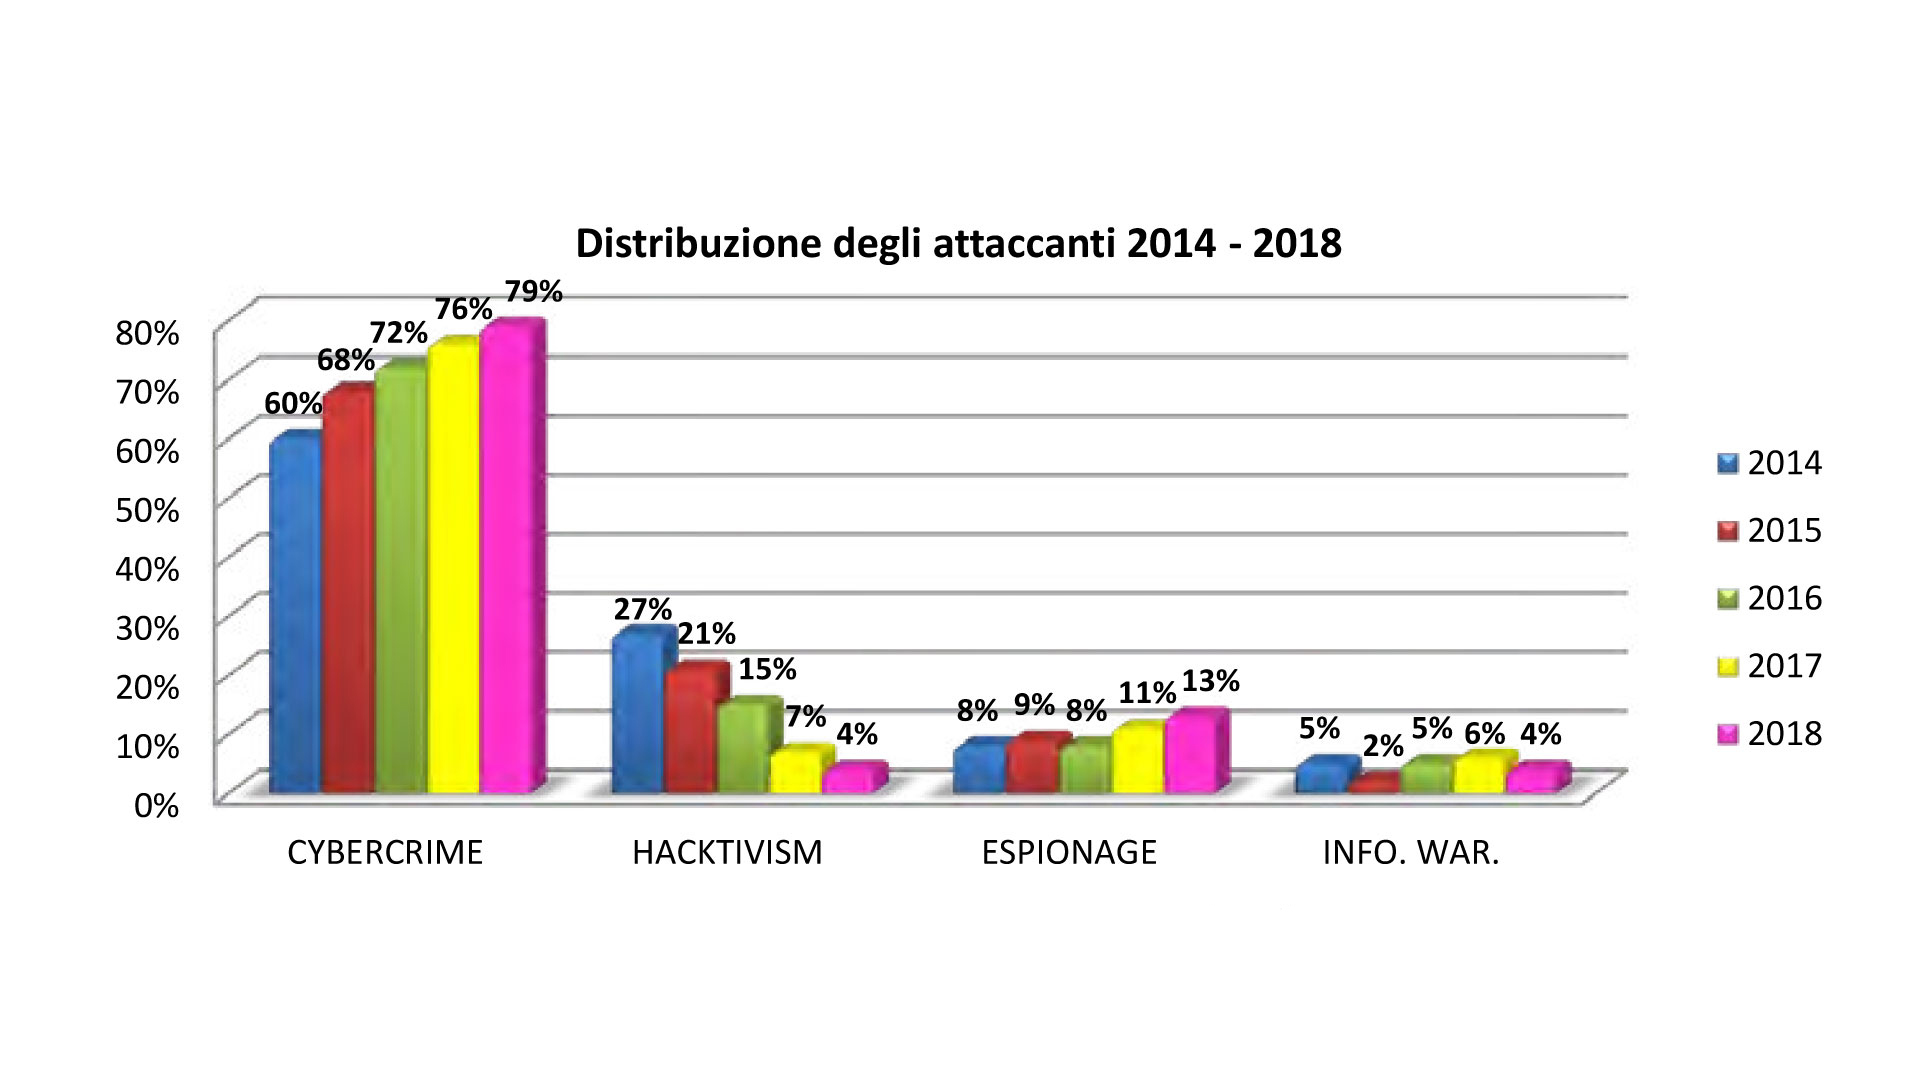
\includegraphics[width=0.8\textwidth]{img/clusit.jpg}
    \caption{Rapporto di distribuzione degli attacchi in ambito ICT in Italia}
    \label{fig:clusit}
\end{figure}

Tali risultati hanno portato all'incremento degli investimenti per aumentare la protezione dei dati e, in generale, rendere i servizi più sicuri. Anche se gli investimenti sono sufficienti, bisogna sempre dover stabilire una infrastruttura di sicurezza che sia efficiente il più possibile per poter preservare i dati in maniera più sicura e trasparente. A ciò, bisogna anche aggiungere anche i costi relativo all'adattamento delle piattaforme verso i criteri di gestione dei dati privati dettati dalla GDPR (General Data Protection Regulator) attiva dal 25 Maggio 2018. 

\newpage
\section{Adattabilità alla GDPR}
La GDPR  è la nuova normativa per la gestione dei dati sensibili e privati propri di un cittadino europeo da parte di aziende private o pubbliche anche se non residenti su suolo europeo. I criteri che riguardano il nuovo regolamento aumentano gli obblighi del titolare del trattamento per garantire la tutela dei dati e i diritti del soggetto interessato. I due aspetti fondamentali sono:

\begin{itemize}
    \item Privacy by design: sin dall'inizio del progetto, bisogna stabilire le misure e le procedure adeguate per garantire la tutela dei dati trattati.
    \item Privacy by default: i dati devono essere trattati con la massima chiarezza, indicando le finalità, le modalità e la durata del trattamento degli stessi.
\end{itemize}

Alla base di tale normativa, vi è l'esplicitazione nell'utilizzo dei dati privati e sotto quali finalità vengono utilizzati, andando ad adottare una politica di gestione il più trasparente possibile. Inoltre, si devono gestire solamente i dati essenziali, ossia si devono raccogliere solamente quei dati che vengono realmente utilizzati all'interno dei servizi offerti, andando a gestirne anche l'aggiornamento in modo da garantire in qualsiasi istante la correttezza. Infine, bisogna tenere un sistema di archiviazione basato sul mantenimento delle informazioni utilizzate recentemente in qualche servizio, rimuovendo tutti i dati obsoleti e non più utili all'interno della piattaforma in cui sono stati utilizzati. 

L'adattabilità a tali requisiti ha portato la diffusione di architetture ICT che si basano sulla trasparenza, sicurezza e la correttezza dei dati. Una delle possibili soluzioni è quella basata sulle tecnologie blockchain che, seguendo il modello private o permissioned, adottano una politica di gestione e archiviazione di dati nel pieno rispetto della GDPR.

\newpage
\voidpage
\chapter{Soluzioni e tecnologie}
All'interno di questo capitolo andremo a definire una spiegazione generale delle tecnologie utilizzate all'interno della soluzione scelta per la gestione dei dati propria dei casi d'uso studiati. Ci soffermeremo inizialmente sulle nozioni che sono alla base, per poi andare a concentrarci sull'utilizzo specifico di un progetto open-source che rappresenta le fondamente dell'architettura presentata all'interno della soluzione, per poi concludere con la spiegazione dell'intera struttura funzionale.
\section{Cos'è una blockchain}
Una blockchain è un registro digitale aperto e distribuito, in grado di memorizzare record di dati (solitamente, denominati "transazioni") in modo sicuro, verificabile e permanente. Una volta scritti, i dati in un blocco non possono essere retroattivamente alterati senza che vengano modificati tutti i blocchi successivi ad esso e ciò, per la natura del protocollo e dello schema di validazione, necessiterebbe del consenso della maggioranza della rete. La blockchain è quindi rappresentabile come una lista, in continua crescita, di blocchi collegati tra loro e resi sicuri mediante l'uso della crittografia. Ad un blocco possono essere associate una o più transazioni e ogni blocco, inoltre, contiene un puntatore hash al blocco precedente e una marca temporale.
La natura distribuita e il modello cooperativo rendono robusto e sicuro il processo di validazione, ma presentano tempi non trascurabili, dovuti in gran parte al processo di validazione dei blocchi e alla sincronizzazione delle rete. L'autenticazione avviene tramite collaborazione di massa ed è alimentata da interessi collettivi. L'utilizzo di questa tecnologia consente anche di superare il problema dell'infinita riproducibilità di un bene digitale e della doppia spesa, senza l'utilizzo di un server centrale o di un'autorità.
Talvolta risulta possibile che alcuni nodi della rete producano simultaneamente più blocchi "concorrenti" (ossia collegati a uno stesso blocco già esistente, ma diversi tra loro nel contenuto): ciò dà origine a una biforcazione (fork) nella catena. Il protocollo di aggiornamento specifica quale regola i nodi debbano adottare per selezionare il blocco da accettare, tra quelli concorrenti. I blocchi non selezionati per l'inclusione nella catena sono chiamati blocchi orfani.
\section{Storia delle blockchain}
Mentre Bitcoin ha solo dieci anni, le origini della tecnologia blockchain sottostante ad esso, e ad altre migliaia di altre criptovalute, risalgono al 1991. Due scienziati hanno trovato un modo per utilizzare la crittografia per il timestamp di file digitali senza il rischio di manomissioni o retrodatazioni. Un anno dopo, è stato progettato un metodo efficiente per la raccolta di documenti in un blocco.
Questi metodi non avrebbero ottenuto un’applicazione significativa fino al 2004, quando lo scienziato informatico Hal Finney ha introdotto il concetto di proof-of-work token, che possono essere trasferiti da persona a persona. Questo concetto, ampiamente considerato come un primo prototipo di Bitcoin, risolse il problema della spesa doppia che esisteva in quel momento nelle soluzioni per le valute digitali.
Il 31 ottobre 2008 Satoshi Nakamoto ha introdotto un sistema di pagamento elettronico peer-to-peer decentralizzato chiamato Bitcoin. (Anche se fino ad ora, l’identità di Satoshi rimane un mistero). Il primo Bitcoin è stato quindi creato tramite mining, sempre da Satoshi, il 3 gennaio 2009. Satoshi ha quindi inviato 10 bitcoin a Hal il 12 gennaio 2009 — la prima transazione di Bitcoin al mondo.
Da lì sono emersi una manciata di progetti blockchain, uno dei quali ha portato alla creazione di varie criptovalute che fungono da alternative al Bitcoin. Nel 2013, il programmatore Vitalik Buterin ha iniziato a sviluppare Ethereum, una nuova piattaforma di calcolo distribuito basata sulla blockchain che consente la creazione di programmi o script, chiamati smart contract, nonché applicazioni decentralizzate. Una criptovaluta chiamata Ether viene utilizzata per pagare le transazioni sulla blockchain di Ethereum.
\newpage
\section{Distributed Ledger Tecnologies}
\begin{figure}[h]
    \centering
    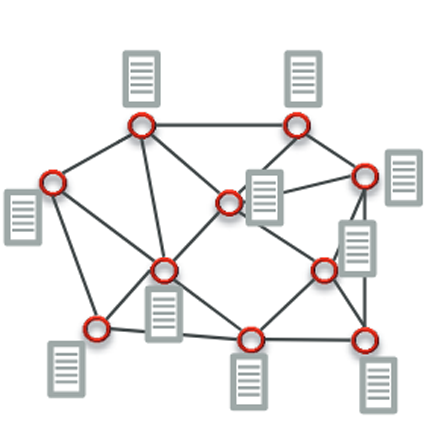
\includegraphics[width=0.5\textwidth]{img/dlt.png}
    \caption{Schema architettura di un distributed ledger}
    \label{fig:dlt}
\end{figure}

L'architettura di rete a cui fanno riferimento le blockchain moderne è basata su un Distributed Ledger. Tale architettura vede i vari nodi della rete collegati tra di loro secondo un'ottica basata sulla distribuzione di risorse, ossia su una decentralizzazione delle funzionalità di gestione dei dati basato su un archivio distribuito. Tale struttura non prevede nessuna organizzazione o entità di validazione dei dati centralizzati, questo aspetto garantisce sicurezza contro possibili alterazione di tale componente, garantendo cosi un livello di protezione implicito intrinseco proprio dell'architettura. Poichè non vi è nessuna validazione centralizzata, per poter definire se un dato sia corretto o meno, si ci avvale di un meccanismo di consenso che vede la partecipazione di più nodi attraverso un processo di votazione, che prevede la validazione o meno di una struttura dati. Le Distributed Ledger Tecnologies si basano proprio sulla gestione del meccanismo del consenso che, all'interno della logica di impostazione del registro decentralizzato,  archivia i dati contenuti all'interno della rete. L'adattabilità di tale logica all'interno del contesto su cui sono basate le blockchain, si ha con la validazione di un nuovo blocco da inserire all'interno della catena. Ogni blocco è formato da una o più transazioni che vengono effettuate all'interno della rete, se il blocco è valido per la maggior parte dei nodi della rete, esso è inserito all'interno della catena e diventa una struttura inalterabile. Il meccanismo del consenso delle DLT viene utilizzato dalla blockchain anche in caso di "forking" della catena, che prevedono il selezionamento di un blocco tra quelli proposti all'interno della rete e si avvalgono del sistema di validazione decentralizzato per poter selezionarne uno tra le possibili scelte ed inserirlo all'interno della catena. 
\section{Tipi di blockchain}
Dopo aver spiegato cos'è una blockchain, quali sono le componenti di base e come essa è strutturata, possiamo ora definire i vari tipi di blockchain che vengono utilizzate oggigiorno all'interno di vari progetti ICT. 
Le blockchain sono, essenzialmente, di tre tipi differenti: private, permissioned e public.
\subsection{Permissioned blockchain}
Le Blockchain permissioned sono soggette ad un’autorità centrale che determina chi possa accedervi. Oltre a definire chi è autorizzato a far parte della rete, tale autorità definisce quali sono i ruoli che un utente può ricoprire all’interno della stessa, definendo anche regole sulla visibilità dei dati registrati. Tali aspetti possono essere utili in molti casi d'uso; in cui si garantisce una gestione gerarchizzata o filtrata delle informazioni dei registri distribuiti, dove si possono definire dati che possono essere pubblici (visibili a tutti i nodi della rete) oppure privati (visibili solamente ad alcuni nodi, quest'ultimo tipo di dati può essere filtrato e reso visibile solamente da una categoria di nodi aventi particolari caratteristiche). Le Blockchain permissioned introducono, quindi, il concetto di centralizzazione della gestione dei dati su un'architettura basata, però, su aspetti come la decentralizzazione e la distribuzione erecditate dalle architetture DLT su cui si basano le blockchain. Quest'ultima caratteristica è molto utile per ridurre i costi di validazione. Infine, il meccanismo del consenso interessa solo un sottoinsieme di nodi e non tutti quelli della rete, la selezione di quali nodi abbiano il diritto di partecipazione al consenso è collegata ai criteri interni alla blockchain. 
\subsection{Private blockchain}
\begin{figure}[h]
    \centering
    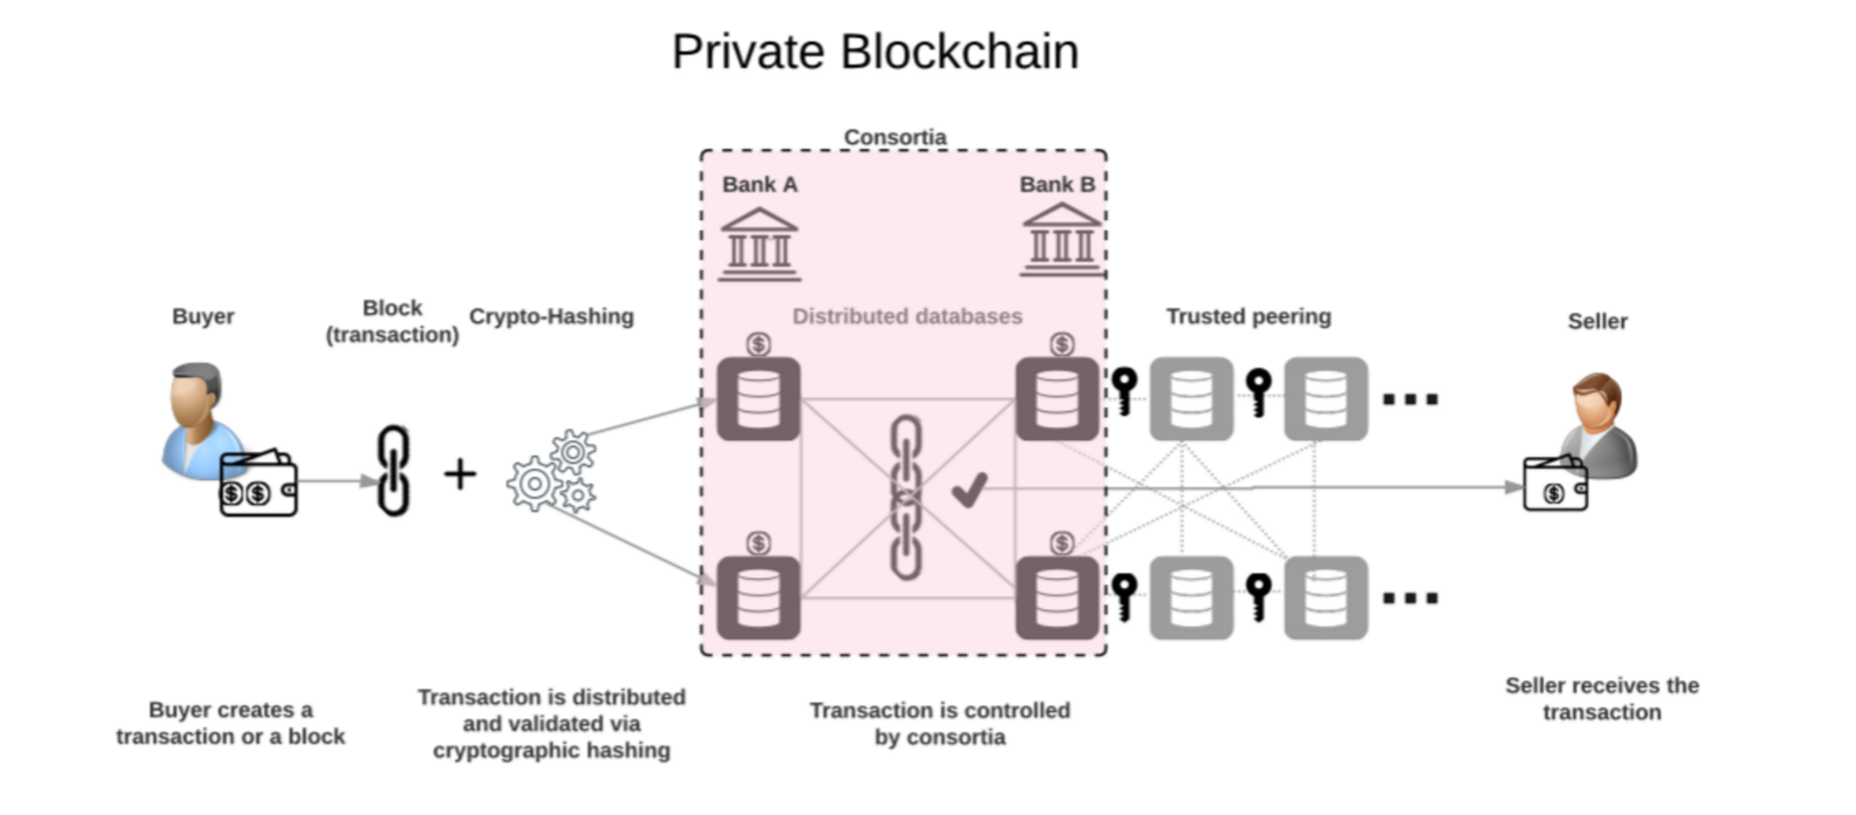
\includegraphics[width=1\textwidth]{img/private-blockchain.png}
    \caption{Caso d'uso di una transazioni in una private blockchain}
    \label{fig:private-blockchain}
\end{figure}
Le blockchain private condividono alcune caratteristiche con le blockchain permissioned. Questo tipo di blockchain viene controllata da una organizzazione centrale che ha la funzione di gestire gli accessi in rete da parte dei vari nodi che tentano di inserirsi. Tale organizzazione è formata da nodi affidabili che vengono ritenuti sicuri e attendibili. Questa organizzazione è alla base non solo della gestione degli accessi, ma anche della manipolazione delle regole di amministrazione dei dati. Quindi, vediamo che tale organizzazione ha la possibilità di variare le regole di gestione delle informazioni contenute nei nuovi blocchi che vogliono aggiungersi alla catena; ossia possono manipolare liberamente le regole di validazione delle transazioni effettuate dai nodi della blockchain
\subsection{Public blockchain}
\begin{figure}[h]
    \centering
    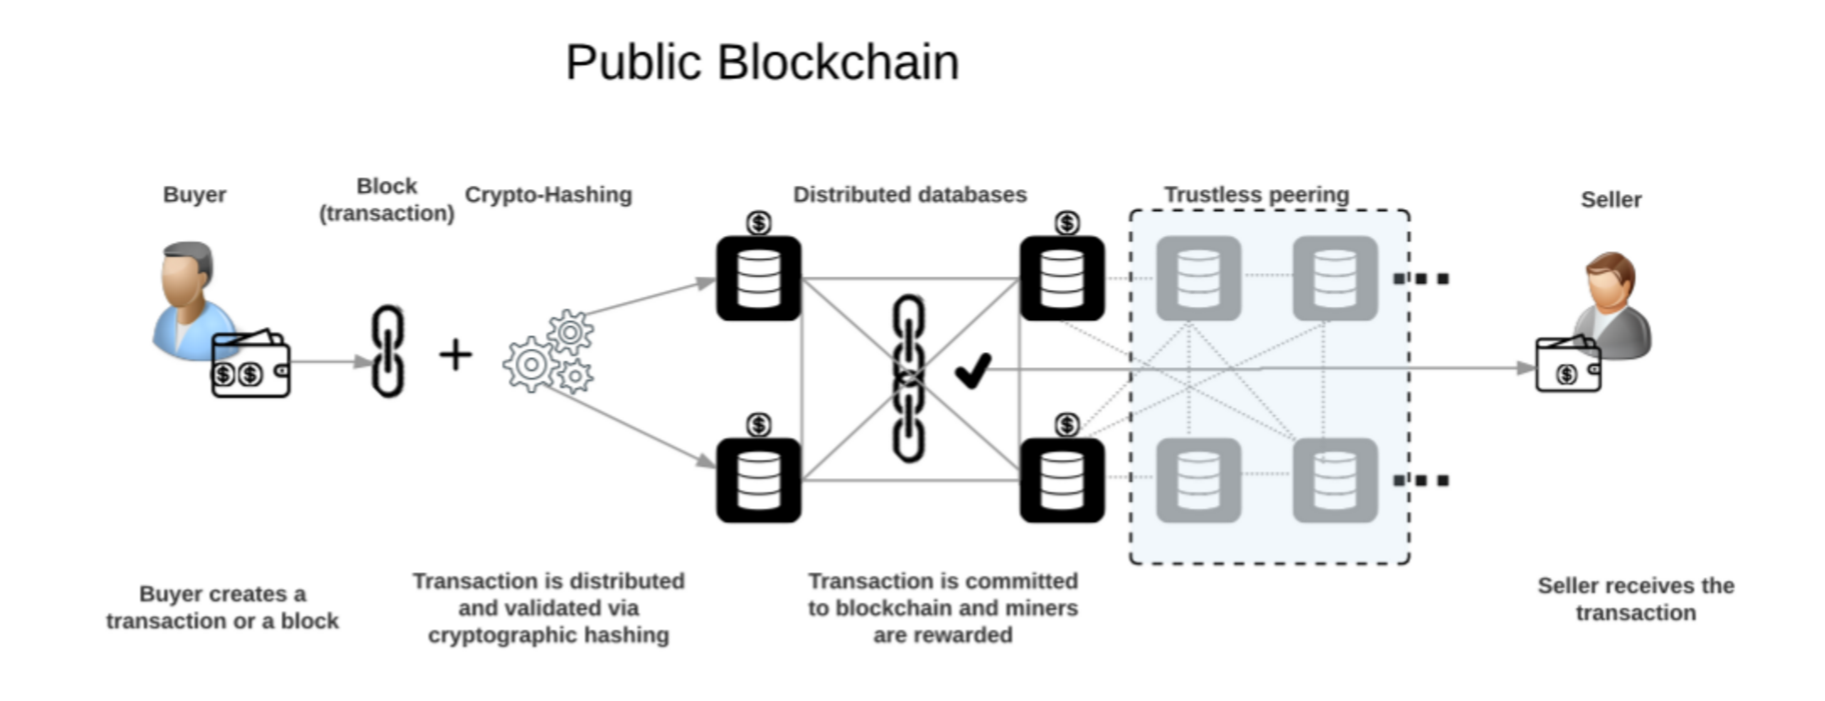
\includegraphics[width=1\textwidth]{img/public-blockchain.png}
    \caption{Caso d'uso di una transazioni in una public blockchain}
    \label{fig:public-blockchain}
\end{figure}
Le public o permissionless blockchain sono essenzialmente il modello principale che raffigura una rete accessibile da chiunque, senza nessuna forma di autorizzazione o autenticazione. Ogni nodo della rete può ricevere o mandare delle transazioni. Ogni nodo è messo allo stesso livello di tutti gli altri della rete, andando a rispettare la natura distribuita della DLT su cui si basano le blockchain. Quando si genera una transazione o si genera un blocco, esso viene sottoposto alla validazione decentralizzata basata sul meccanismo di consenso. Quindi, vediamo che i nodi della rete hanno principalmente due ruoli fondamentali: Il primo è quello di generare o ricevere le transazioni da o verso la blockchain, il secondo è quello di partecipare al meccanismo di validazione delle varie transazioni che andranno ad essere inserite all'interno dei blocchi che andranno a costituire la catena. 
\section{Procedimento di creazione di un blocco}
Come spiegato precedentemente, quando si effettuano delle operazioni su dati all'interno dell'archivio distribuito mantenuto nella blockchain, si ha una transazione. Dopo la sua creazione, una transazione viene inserita in un blocco che deve essere validato da una serie di nodi denominati miner. I miner sono quei nodi che sono adibiti alla verifica di un blocco. Il processo di validazione di un blocco si concentra su un'operazione di ricerca di un valore che, se aggiunto ad altre informazioni del blocco sotto analisi, restituisca un determinato codice hash. La ricerca di tale valore è concorrente tra i vari miner interessati nel processo di verifica che competono per ritrovare tale valore corretto. Quando uno dei vari miner riesce a trovare il valore richiesto, si passa ad una fase di verifica da parte di tutti gli altri miner per certificare la correttezza del risultato. In caso affermativo, il miner che ha trovato il risultato desiderato riceve, in genere, un token. Tale token può essere una moneta virtuale come i Bitcoin. Il processo di verifica della correttezza del valore da parte di tutti gli altri miner interessati nella validazione viene definito come proof-of-work o PoW. In seguito, il blocco verificato viene aggiunto alla catena che identifica la blockchain aumentando cosi la sua lunghezza.
\newpage
\subsection{Funzione di Hash}
\begin{figure}[h]
    \centering
    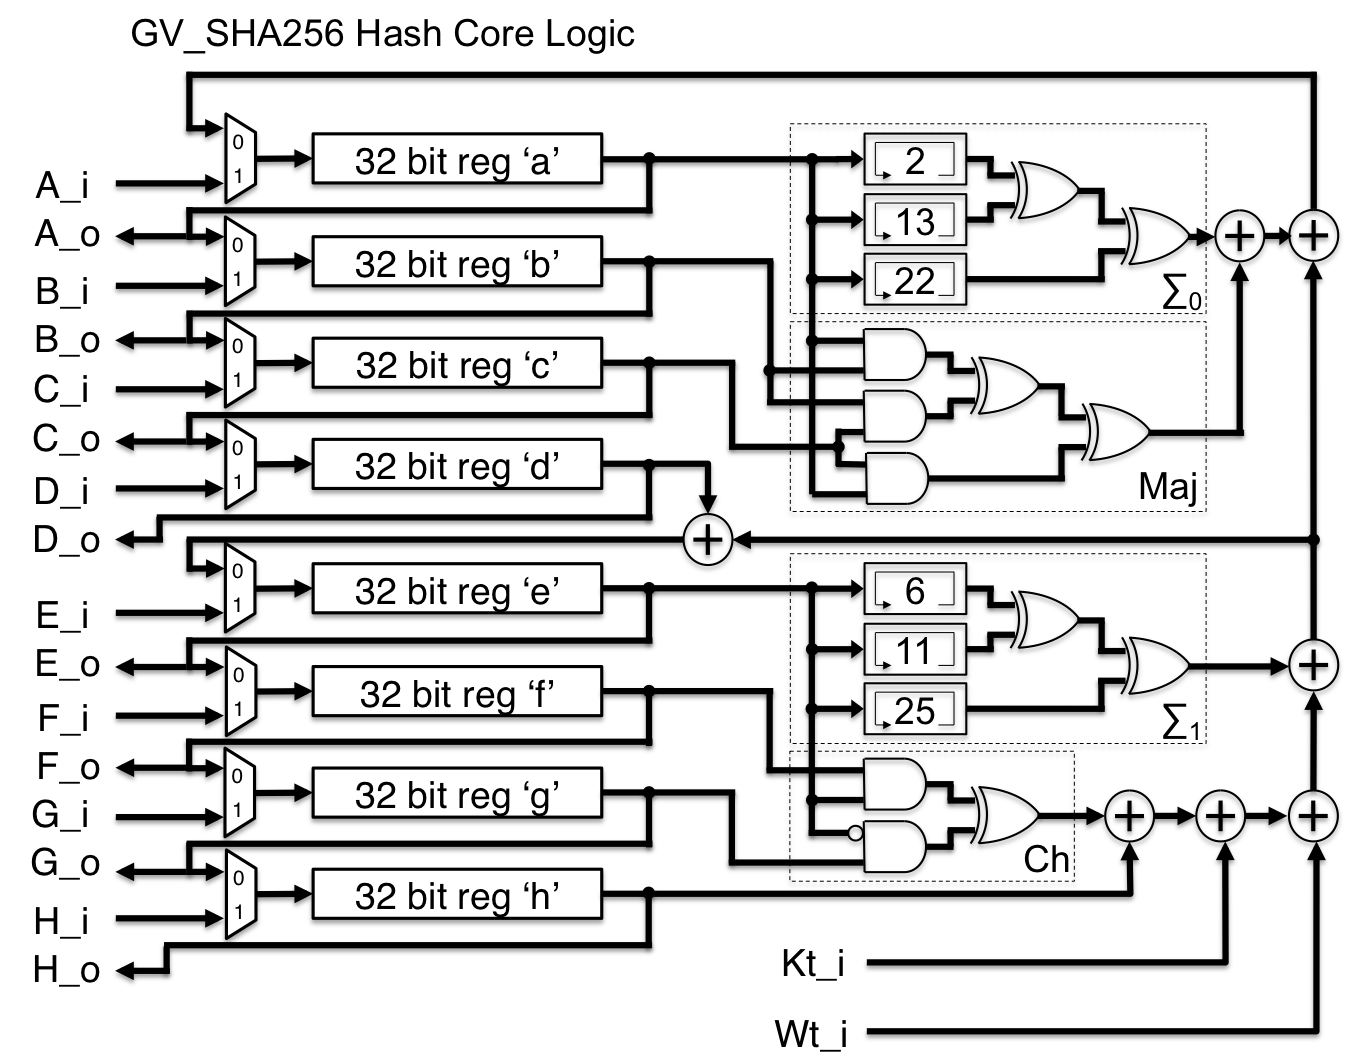
\includegraphics[width=0.78\textwidth]{img/sha256.png}
    \caption{Logica Hash Code SHA-256}
    \label{fig:sha256}
\end{figure}
La ricerca del valore e la generazione di un codice hash viene definito secondo un particolare algoritmo di crittografia. All'interno delle blockchain moderne, secondo una visione ad alto livello, l'algoritmo di hash prende in input una serie di dati che possono essere di lunghezza variabile e, tramite una funzione di hash, si ha la conversione ad una stringa di caratteri di lunghezza predefinita raffigurante l'output della funzione. Tale procedimento è irriversibile, nel senso che non è possibile risalire alla stringa di input partendo da quella di output. Generalmente, la funzione di hash che si utilizza all'interno di una blockchain è lo SHA-256, esso usa una funzione che restituisce sempre una stringa di lunghezza fissa pari a 256 bit. Il procedimento di ricerca prevede di applicare una serie di operazioni in cui si specificano una successione di tentativi di input, una conversione di quest'ultimo alla stringa hash corrispondente e una verifica andando a confrontarla con la stringa codificata da decifrare. Se la codifica dell'input e la stringa ricercata combaciano, allora si è trovato il valore ricercato. Notiamo che dato uno specifico input, si avrà sempre un medesimo output ad ogni conversione effettuata. La difficoltà nel trovare una possibile stringa di input partendo dalla stringa di output è alla base della gestione dello SHA-256. Questo perchè vi sono al più una possibile combinazione che potrebbero corrispondere alla stringa di input ricercata. Inoltre, vediamo che non vi è nessun criterio ancora conosciuto su come tale funzione hash possa essere prevista se non tramite algoritmi di risoluzione basati sulla brute-force. Lo SHA-256 è alla base della crittografia moderna, andando ad essere applicato su qualsiasi forma di sicurezza e mascheramento di dati all'interno dell'ambito ICT. 
\section{Applicazione della funzione Hash}
Più nello specifico, nell'applicazione della funzione hash, si ha che i miner di una blockchain sfruttano il loro poter computazionale per trovare un numero (chiamato nonce). Questo, se processato tramite la funzione di hash, insieme ad altri dati presenti nel blocco da validare, deve restituire un risultato codificato che inizia con un determinato numero di zeri. Questo codice viene chiamato "hash della testa del blocco". Il numero di zeri richiesti definisce il grado di difficoltà per la validazione del blocco, in quanto maggiore è il numero di zeri e maggiore è la difficoltà di validazione (il numero di zeri richiesti è definito in uno dei dati presenti nel blocco). Quindi lo scopo principale per la validazione di un blocco è quella di trovare un nonce in modo tale che, aggiunto agli altri dati del blocco ci dia come risultato la stringa hash in SHA-256 corrispondente. Non esiste una tecnica o un calcolo per trovare un nonce valido, l'unico modo logico per farlo è tramite numerosi tentativi casuali. Proprio per questo motivo, i miner si servono di appositi hardware che misurano la loro potenza in "tentativi al secondo" (H/s). Da qui nasce il concetto di "competizione tra miner", in quanto solo il miner che troverà per primo un nonce valido verrà ricompensato per il lavoro svolto. Prima di essere ricompensato però, il miner che trova un nonce valido comunica la soluzione agli altri nodi della rete, questi effettueranno una verifica per confermare che il nonce sia valido. Qualora il nonce non fosse valido, la competizione si riapre e tutti i miner tornano alla ricerca del medesimo nonce.
\newpage
\section{Crittografia asimmetrica e gestione delle criptovalute}
La crittografia asimmetrica si basa sull'utilizzo di una coppia di chiavi: Una pubblica e una privata. La chiave pubblica è visibile a tutti i nodi di una rete, che possono sfruttarla per criptare un dato all'interno di una trasmissione, la chiave privata è propria di ogni nodo, quindi non è condivisa con gli altri dispositivi della rete; essa serve per decriptare un messaggio o un dato trasmesso all'interno del network. Quando un messaggio viene criptato tramite una chiave pubblica, esso potrà successivamente essere decriptato solamente dal possessore della chiave privata corrispondente. Tale aspetto, fa si che qualsiasi dispositivo possa criptare il nodo e solamente quello proprietario possa decriptarlo. Facciamo un esempio per chiarire quanto appena detto. Abbiamo due persone: A e B. A vuole inviare un documento di testo a B, ma vuole accertarsi del fatto che solo B sia in grado di leggere il contenuto di tale documento. A decide allora di utilizzare la crittografia asimmetrica, si serve quindi della chiave pubblica di B per criptare il suo messaggio (A conosce la chiave pubblica di B in quanto, essendo appunto pubblica, B l'ha messa a disposizione di A). Il documento così criptato non è più decifrabile da A, in quanto non è in possesso della chiave privata di B (questa, al contrario della chiave pubblica, è appunto privata: solo B ne è in possesso). B riceve il documento e riesce a decifrarlo utilizzando la sua chiave privata. 


\begin{figure}[h]
    \centering
    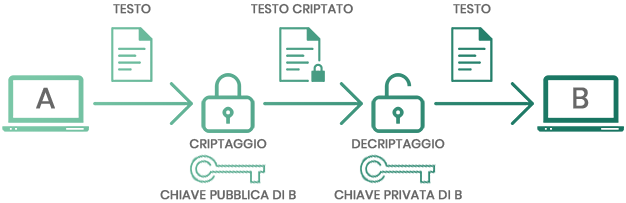
\includegraphics[width=0.78\textwidth]{img/asymmetric-cripto.png}
    \caption{Simulazione di crittografia asimmetrica}
    \label{fig:asimmetric-crypto}
\end{figure}
Vediamo ora come tale procedura viene utilizzata all'interno di una blockchain. La crittografia asimmetrica viene utilizzata all'interno della gestione di una transazione che vede il trasferimento tra due account di una criptovaluta o di dati da o verso un'account. Notiamo che una delle principali caratteristiche che si hanno sulla transazione è come essa viene trasferita. Secondo uno schema standard, si distingue l'account mandante da quello ricevente. All'interno della transazione si fa uso della chiave privata e pubblica del ricevente. Quando si effettua una transazione, il mandante cripta utilizzando la chiave pubblica del ricevente, tale procedimento è possibile poichè la chiave è all'interno delle informazioni note del mandante. In seguito, la transazione può essere decriptata solamente dal ricevente, questo perchè se si effettua un'operazione di criptaggio utilizzando una chiave pubblica, essa può essere decriptata solamente dalla rispettiva chiave privata che, come detto precedentemente, è propria solamente dell'account possessore che, in questo caso, è l'account ricevente. Quando si ha una transazione incentrata sul trasferimento di una criptovaluta, il procedimento sussiste anche nell'estrazione e nel deposito sui wallet degli account interessati. I wallet sono dei "portafogli virtuali" che mantengono solamente traccia della transazione mentre le criptovalute sono mantenute all'interno del ledger su cui si fonda la blockchain.

\section{Proof-of-Work}
Il concetto originale di Proof-of-Work risale al 1993, anno in cui è stato sviluppato per prevenire attacchi denial of service e altre violazioni come network spam. Sostanzialmente questa soluzione richiedeva un po’ di lavoro all’utente del servizio, inteso come tempo di lavorazione di un computer.
Nel 2009, Bitcoin ha introdotto un metodo innovativo per utilizzare la Proof-of-Work come algoritmo di consenso per convalidare transazioni e trasmettere nuovi blocchi alla blockchain. 
Da allora si è diffuso fino a diventare un algoritmo di consenso ampiamente utilizzato nelle blockchain. Il Proof-Of-Work si basa su due operazioni fondamentali:
\begin{enumerate}
    \item Risoluzione di enigmi computazionali: Difficile da ottenere, si sfrutta il potere computazionale per trovare il valore corrispondente ad una stringa hash. Dato che la funzione di hash è irreversibile, la ricerca della soluzione ha una complessità computazionale basata su una ricerca in brute-force.
    \item Verifica della soluzione: Facile da ottenere, non si fa altro che applicare sul valore risultato la funzione di hash e verificare che l'output sia quello corretto.
\end{enumerate}
In sintesi, i miner all’interno di una rete competono tra di loro per risolvere enigmi computazionali complessi. E’ difficile trovare la soluzione di questi enigmi, ma allo stesso tempo è facile verificare se questa è corretta. Quando un miner trova la soluzione a un'enigma, può trasmettere il blocco alla rete, e tutti gli altri miner verificano che la soluzione sia effettivamente corretta.
\section{Proof-of-Stake}
L’algoritmo Proof-Of-Stake utilizza un processo di elezione pseudo-casuale per selezionare un nodo che agirà da validatore univoco del blocco successivo, in base a una combinazione di fattori che possono includere periodo di staking, randomizzazione e fondi di proprietà del nodo. L'algoritmo di selezionamento del nodo è variabile e definisce varie forme che, sotto un punto di vista procedurale, varia solamente per l'aspetto di selezionamento.
\subsection{Forging}
E’ bene osservare che, nei sistemi Proof-of-Stake, l’inserimento di nuovi blocchi nella blockchain viene chiamato con il termine di forging invece che di mining, quindi i blocchi vengono 'forgiati'. Una buona parte delle criptovalute che utilizzano la Proof-of-Stake iniziano vendendo monete pre-minate, oppure sfruttano l’algoritmo Proof-of-Work e in seguito passano alla Proof-of-Stake.
Mentre nei sistemi basati sulla Proof-of-Work viene creata nuova moneta per ricompensare i miner, generalmente il sistema Proof-of-Stake distribuisce come premio solo le commissioni sulle transazioni.
Gli utenti che vogliono partecipare al processo di forging devono congelare una certa somma di monete all’interno del network, mettendo quindi un’adeguata posta in gioco. Le dimensioni della stake, ossia le criptovalute messe in gioco, determinano le probabilità di un nodo di venir selezionato come validatore e agire da forger del blocco successivo - più grande la stake, maggiori le probabilità. Tuttavia, per fare in modo che questo processo non favorisca solo i nodi più ricchi del network, il processo di selezione presenta altri metodi unici. I più comuni sono ‘Randomised Block Selection’ e ‘Coin Age Selection’.
\newpage
\subsection{Randomised Block Selection}
Con il metodo Randomised Block Selection, i validatori vengono selezionati cercando i nodi con una combinazione tra valore hash più basso e stake più grande. Dato che le dimensioni delle stake sono pubbliche, in genere gli altri nodi possono prevedere quale verrà selezionato.
\subsection{Coin Age Selection}
Il metodo Coin Age Selection sceglie nodi in base a quanto tempo hanno lasciato i propri token congelati come stake. La coin age viene calcolata moltiplicando il numero di giorni per il numero di monete congelate. Quando un nodo forgia un blocco, la sua coin age viene resettata a zero e deve aspettare un certo periodo di tempo prima di poter essere selezionato - questo impedisce ai nodi con grandi stake di dominare la blockchain.
\subsection{Inserimento di un blocco tramite Proof of Stake}
Ogni criptovaluta che usa l’algoritmo Proof of Stake presenta una propria lista di regole e metodi per creare la migliore combinazione possibile per il network e per gli utenti.
Quando un nodo viene selezionato come forger del blocco successivo, deve controllare se le transazioni in esso contenute sono valide, firmare il blocco e aggiungerlo alla blockchain. Come ricompensa, il nodo riceve le commissioni associate alle transazioni nel blocco.
Se un nodo vuole smettere di partecipare al processo di forging, deve attendere un certo periodo di tempo prima di poter accedere alla propria stake e alle ricompense guadagnate, lasciando al network tempo per verificare che non abbia aggiunto blocchi fraudolenti alla blockchain. La stake funge da incentivo economico che dissuade il nodo forger dal convalidare o creare transazioni fraudolenti. Se il network individua una transazione fraudolenta, il nodo forger perde parte della sua stake, oltre al diritto a partecipare come forger in futuro. Quindi, a patto che la stake sia più grande della ricompensa, il validatore che tenta di raggirare il sistema perderebbe molto di più rispetto a quello che riuscirebbe a guadagnare. Per riuscire a raggiungere un controllo effettivo del network e approvare transazioni fraudolente, un nodo dovrebbe possedere una stake maggioritaria, situazione conosciuta come 51\% attack. A seconda del valore di una criptovaluta, un attacco del genere risulta quasi irrealizzabile dato che per ottenere il controllo del network sarebbe necessario acquisire il 51\% delle unità in circolazione.I vantaggi principali dell’algoritmo Proof of Stake sono l’efficienza energetica e la sicurezza. La facilità e l’accessibilità incoraggia un maggior numero di utenti a impostare e mantenere nodi. Questo, insieme al processo di randomizzazione, rende il network più decentralizzato, in quanto non sono più necessarie mining pool per aggiungere blocchi. Inoltre, dato che non vengono più distribuite nuove monete come ricompensa, il prezzo di una particolare moneta rimane più stabile.
\subsection{Utilità del Proof-of-Stake}
In conclusione, una delle caratteristiche principali che delineano l'utilizzo del Proof-of-Stake rispetto al meccanismo delineato dal Proof-of-Work è che nel primo caso si ha una utilità di natura transazionale, il forger scelto non fa altro che delineare una ricompensa solamente per essere stato selezionato nella convalida di un blocco senza creare la criptovaluta guadagnata ma utilizzarne una pre-minata, ciò ha come vantaggio non solo quello di definire un meccanismo di premiazione ben concisa, ma riesce anche ad evitare lo sforzo computazionale che si aveva nel Proof-of-Work.
\newpage
\section{Smart Contract}
Uno smart contract è un vero e proprio contratto in codice, scritto su una blockchain. Questo viene utilizzato per regolamentare una transazione tra due o più parti. Questo contratto viene definito intelligente (smart), in quanto è in grado di verificare se determinate condizioni, definite alla base (nel codice) del contratto stesso, sono avvenute ed è in grado di eseguirsi automaticamente - portando a termine la transazione tra le parti - nel momento in cui tali condizioni sono state raggiunte e/o verificate.
La funzione alla base di uno smart contract è in grado di leggere sia le condizioni che le clausule concordate nel contratto: non appena i dati riferiti a situazioni reali corrispondono alle condizioni e ai dati riferiti nelle clausule concordate, il contratto intelligente viene eseguito, portando a termine la transazione tra le parti.
Nella stesura e creazione di uno smart contract bisogna essere estremamente precisi. Le parti che sottoscrivono il contratto devono scegliere con cura le condizioni, le clausule e le fonti di dati su cui il contratto è chiamato ad attenersi. Lo smart contract è quindi un programma che elabora, in maniera deterministica, le informazioni che vengono raccolte, in questo modo si ha la certezza di un giudizio oggettivo, escludendo inevitabilmente qualsiasi forma di interpretazione.
\begin{figure}[h]
    \centering
    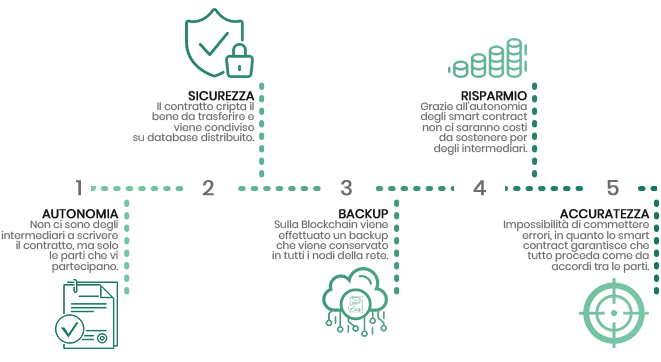
\includegraphics[width=0.9\textwidth]{img/smart-contract.png}
    \caption{Vantaggi derivati dall'uso di uno smart contract}
    \label{fig:smart-contract}
\end{figure}
Grazie agli smart contract è finalmente possibile eliminare qualsiasi tipo di intermediario e i costi a essi associati, in quanto non potrà mai esistere qualcosa o qualcuno che sia più preciso e affidabile di uno smart contract.
Ai contraenti spetta il compito di definire le condizioni, le clausole, le modalità, le regole di controllo e di azione, ma una volta che il contratto è stato scritto e accettato, i contraenti non potranno in alcun modo modificare o annullare la transazione. Gli effetti della transazione non dipendono più dalla volontà dei contraenti, in quanto sarà il contratto a portare a termine il tutto senza soggettività, così come è stato definito nel contratto in maniera completamente sicura e trasparente.
\section{Forking}
Una delle caratteristiche che raffigurano un software generico è la necessità di aggiornamenti. Tali aggiornamenti possono rappresentare delle modifiche da apportare all'interno delle regole di gestione dei dati come cambiamenti sulle regole di validazione di un blocco all'interno delle blockchain, la sua dimensione, le modalità di gestione delle ricompense o la tipologia di cryptovaluta utilizzata. In generale, quando si parla di regole si fa sempre riferimento ad un protocollo che, nel contesto delle blockchain, si riferiscono alla gestione dei blocchi e dei dati all'interno dei vari nodi della rete. La gestione degli aggiornamenti all'interno di una blockchain viene definito con il termine di forking. Esistono due tipologie di forking: Soft fork e Hard fork, in entrambi i casi vi è una modifica del protocollo, la differenza sostanziale si vede nella convalida dei blocchi e come vengono gestiti i consensi o le negazione da parte dei nodi aggiornati al nuovo protocollo e quelli ancora con la versione precedente.
\subsection{Soft fork}
Le soft fork sono delle modifiche retro-compatibili, ossia delle modifiche in cui la versione aggiornata e quella precedente hanno nella loro definizione delle caratteristiche non contrastanti. Tale aspetto ha come risultato quello di poter far elaborare nuove transazioni e aggiungere nuovi blocchi alla catena da parte dei nodi che ancora non hanno subito l'aggiornamento del protocollo se le proprietà dei nuovi blocchi rispettano le regole della nuova versione.
\begin{figure}[h]
    \centering
    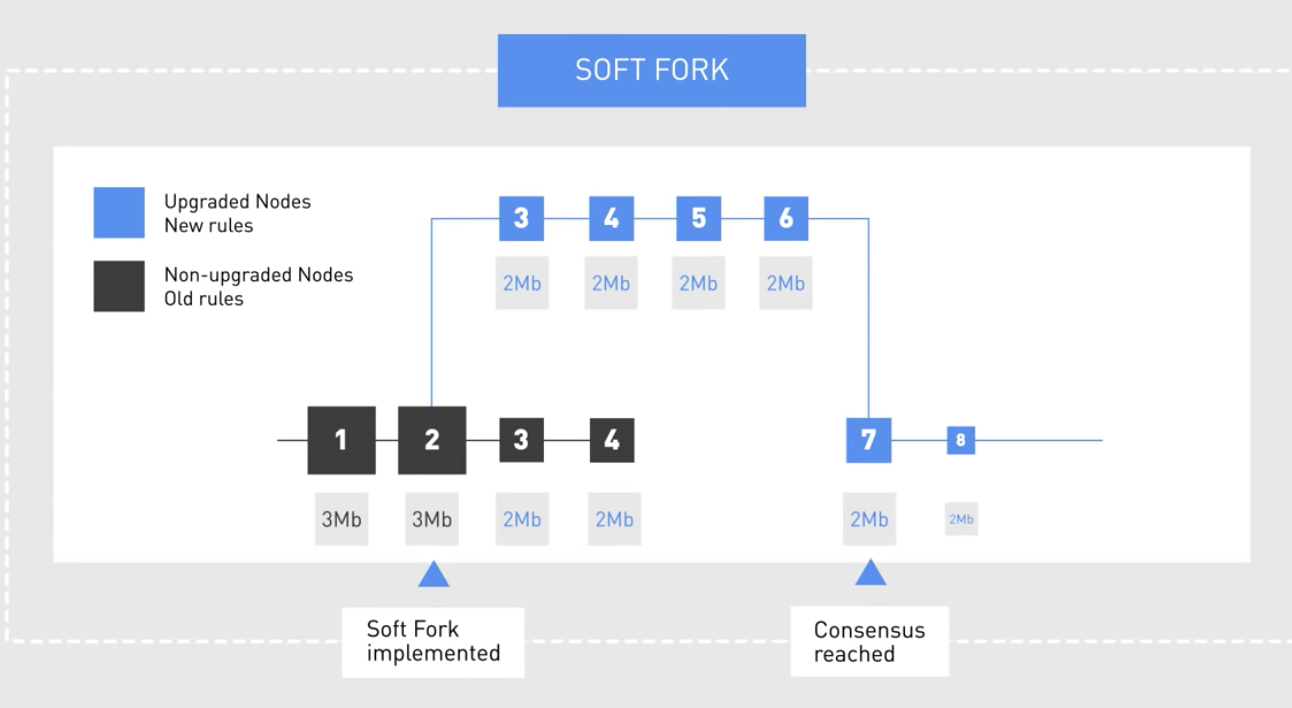
\includegraphics[width=0.8\textwidth]{img/soft-fork.png}
    \caption{Procedura di soft fork}
    \label{fig:soft-fork}
\end{figure}
Un esempio di soft fork si può avere nella modifica del protocollo sulla grandezza del blocco da aggiungere alla catena. Se si ha una riduzione della dimensione da 3 MB a 2 MB e i nodi non aggiornati producono un blocco con dimensione pari o non superiori a 2 MB, essi vengono comunque validati da parte dei nodi aggiornati poichè rispettano ugualmente le proprietà delle nuove regole del protocollo. Se invece producono un blocco superiore a 2 MB, esso verrà rifiutato poichè non conforme secondo le regole dei nodi aggiornati.
\subsection{Hard fork}
Sono delle modifiche che creano delle biforcazioni contrastanti tra di loro poichè l'aggiornamento del protocollo rende incompatibile la versione antecedente rispetto quella attuale, causando l'impossibilità di generare dei nuovi blocchi da parte dei nodi ancora non aventi la versione corrente del protocollo sotto analisi. In genere un hard fork si presenta quando si intende aggiornare ed estendere un protocollo già esistente oppure quando si vuole definire una catena di blocchi indipendente rispetto a quella della versione precedente. 
Immaginando una modifica in un protocollo che aumenta la dimensione dei blocchi da 2 MB a 4 MB. Se un nodo aggiornato prova ad aggiungere un blocco pari a 3 MB nella blockchain, i nodi non aggiornati vedranno tale blocco come non valido, andandolo a rifiutare.
Gli hard fork hanno due forme specifiche:
\begin{enumerate}
    \item Hard fork programmati
    \item Hard fork controversi
\end{enumerate}
\begin{figure}[h]
    \centering
    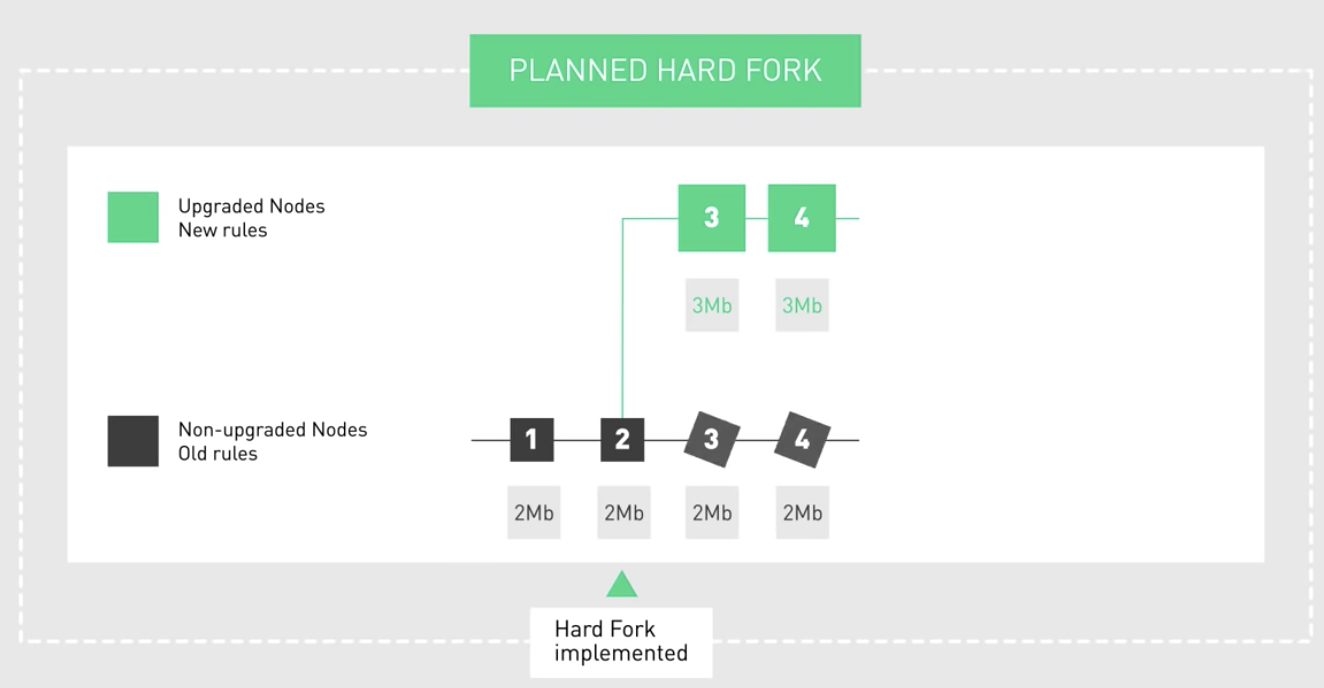
\includegraphics[width=0.8\textwidth]{img/planned-fork.png}
    \caption{Schema di Hard Fork Programmato}
    \label{fig:planned-fork}
\end{figure}
Nel primo caso, i nodi aggiorneranno automaticamente il protocollo, ignorando la vecchia versione. In questo caso, si avrà un forking in cui vede la differenza nel consenso tra i nodi aggiornati e quelli non aggiornati che continueranno ad operare sulla vecchia catena finchè non verranno aggiornati, andando, così, ad abbandonarla definitivamente. Tale forma di hard fork viene effettuata quando tutti i nodi sono d'accordo sulle modifiche da effettuare e, quindi, vi è un'aggiornamento di massa senza nessuna divisione decisoria. 
\begin{figure}[h]
    \centering
    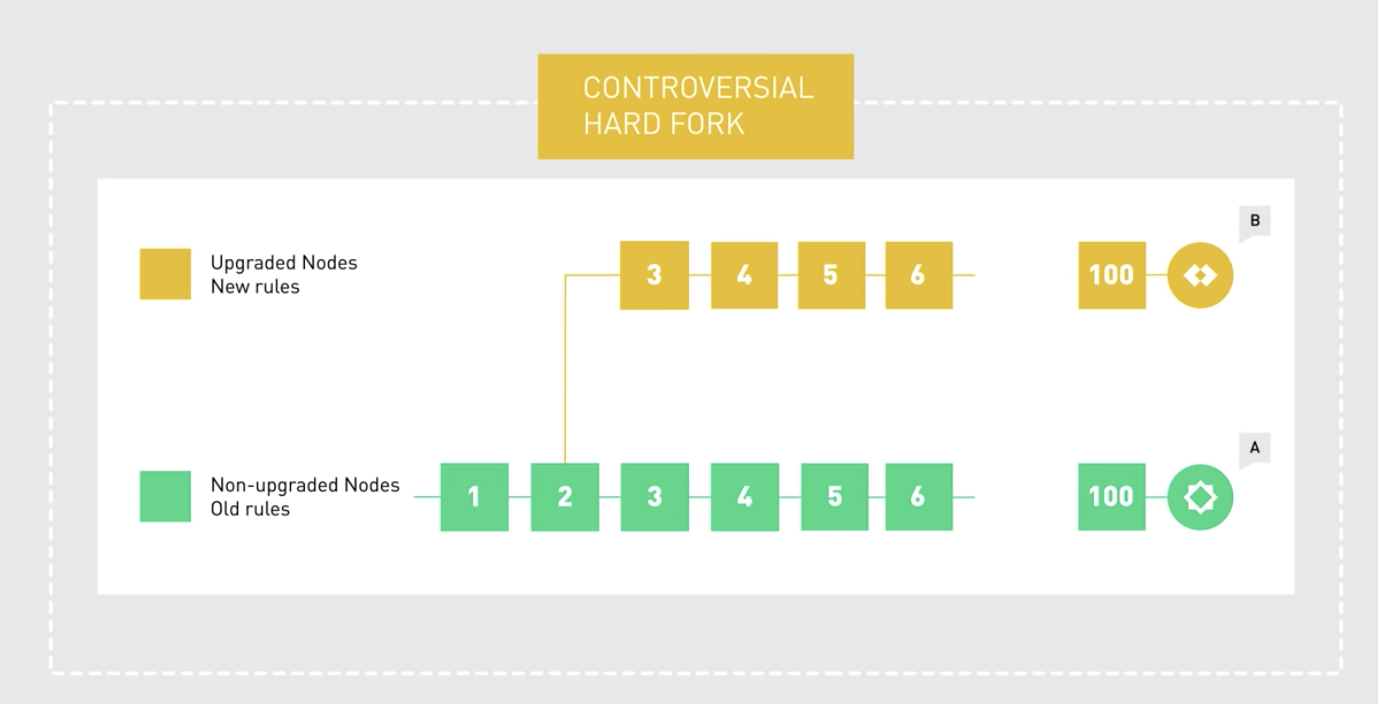
\includegraphics[width=0.8\textwidth]{img/controversial-fork.png}
    \caption{Schema di Hard Fork Controverso}
    \label{fig:controversial-fork}
\end{figure}
Nel secondo caso, la biforcazione si effettua anche sotto un punto di vista di scelta nell'aggiornare o meno il protocollo della blockchain. Con gli hard fork controversi si ha come risultato finale la creazione di due blockchain separate, indipendenti ed incompatibili. Ogni blockchain avrà una propria criptovaluta, i nodi che parteciperanno ad una delle due biforcazioni si distingueranno a secondo dell'aggiornamento o meno del protocollo. 
Dato che un fork si basa sulla blockchain originale, tutte le transazioni che sono state effettuate andranno ad essere copiate nella nuova blockchain. Per esempio, se possiedi 100 monete di una criptovaluta chiamata Moneta A, e un hard fork basato su tale criptovaluta ne crea una nuova chiamata Moneta B, riceverai anche 100 monete della Moneta B. In seguito alla replica delle criptovalute, le due monete diventeranno completamente indipendenti tra di loro, una modifica ad una di esse non comporterà modifiche allo stato dei nodi sull'altra blockchain. Tali biforcazioni sono molto frequenti all'interno del campo di sviluppo delle criptovalute. Un esempio di hard core controverso lo si ha avuto con Ethereum. I questo caso la causa scatenante è stato un attacco informatico verificatosi in una delle loro applicazioni (denominata DAO). Una parte minoritaria della comunità era contraria a cambiare la blockchain ad ogni costo, per preservare la sua natura di immutabilità. Così mentre gli sviluppatori principali di Ethereum e la maggior parte della sua comunità andavano avanti con l’Hard Fork, la minoranza non ha aggiornato il software continuando a estrarre quello che è ora noto come Ethereum Classic.
\newpage
\section{Vantaggi e svantaggi nelle blockchain}
Possiamo ora analizzare le caratteristiche fondamentali proprie delle blockchain, andando a definire i vantaggi e gli svantaggi che si hanno, delineando cosi i vari possibili utilizzi che tale struttura può avere all'interno dell'ambiente ICT. 
\subsection{Vantaggi}
I vantaggi nell'utilizzo di una blockchain si possono ridurre a 3 aspetti principali:
\begin{itemize}
    \item Distributività: i dati in una blockchain sono contenuti all'interno di più copie localizzate nei vari nodi della rete in maniera distribuita. Dato che ciascun nodo è capace di archiviare e copiare una copia del database, guasti relativi a singoli nodi non portano problemi al sistema che, in contesti come quello analizzato, sono intolleranti ai guasti. Inoltre, una volta "riparato" un nodo, è sempre possibile recuperare una copia dell'archivio distribuito interno cosi da poter ristabilire il corretto funzionamento del dispositivo guasto. 
    \item Stabilità: è molto improbabile che i blocchi confermati vengano invertiti e annullati, ciò significa che, una volta che sono stati registrati nella blockchain, i dati sono estremamente difficili da rimuovere o modificare. Questo aspetto rende le blockchain ideali per casi d'uso in cui si ha la necessità di tracciare qualsiasi modifica venga effettuata sul registro distribuito. Casi d'uso esempio che possano garantire tali caratteristiche sono tutti quelli legati ad un monitoraggio dei cambiamenti cosi da poter prendere visione delle transazioni che sono state effettuate andando ad evidenziarne usi non consoni alle funzionalità che si appoggiano su tale architettura. 
    \item Trustless: uno dei punti cardini più importanti che si ha quando si parla di blockchain è data dalla capacità del sistema di gestire i dati in totale sicurezza senza l'ausilio di un intermediario. Questo è garantito anche dal sistema di consenso che riesce a verificare un blocco grazie al Proof of Work o al Proof of Stake, oppure con il rispetto degli smart contract instanziati all'interno dei vari nodi della rete. Un'esempio di caso d'uso incentrato sulla gestione trustless dei dati lo si può avere con i sistemi finanziari decentralizzati che non hanno bisogno di intermediari come banche o servizi di pagamento ma la verificabilità e la correttezza dei dati sono garantiti dai medesimi dispositivi che possono effettuare una transazione finanziaria. 
\end{itemize}
\subsection{Svantaggi}
Per quanto riguarda gli svantaggi, i principali punti a sfavore sulla struttura e la logica di gestione delle  blockchain sono i seguenti:
\begin{itemize}
    \item 51\% attack: Anche se il Proof of Work lavora molto bene per garantire l'affidabilità e la sicurezza sul sistema, vi sono particolari attacchi che possono bypassare tale meccanismo di sicurezza, uno dei più famosi è il 51\% attack. Tale attacco prevede l'appropriazione di più del 50\% della potenza di calcolo complessiva della rete, cosi da garantire un controllo verso la blockchain e gestendo in maniera fraudolenta le transazioni contenute nei vari blocchi della blockchain. Nonostante sia teoricamente possibile, notiamo che le blockchain attualmente attive non hanno mai subito un attacco di tale genere. Inoltre, la probabilità di successo del 51\% attack è inversamente proporzionale alla quantità di dispositivi collegati alla rete e interessati al meccanismo di validazione. Oltre a questo, un 51\% attack di successo riuscirebbe a modificare soltanto le transazioni più recenti per un breve periodo di tempo, in quanto i blocchi sono connessi attraverso prove crittografiche (cambiare blocchi più vecchi richiederebbe livelli di potenza computazionale intangibili).
    \item Difficoltà nel modificare i dati: Notiamo che l'immutabilità dei dati inerenti ad un blocco porta il vantaggio di stabilità all'interno delle blockchain. Tale caratteristica, però, può essere positiva in alcuni casi e negativa in altri. Notiamo che per modificare un blocco all'interno di una blockchain c'è bisogno di effettuare un hard fork andando ad abbandonare una catena per sostituirne un'altra. 
    \item Chiavi private: Le blockchain utilizzano un meccanismo asincrono di criptaggio gestito attraverso l'utilizzo di chiave pubblica e chiave privata. Ogni account sulla blockchain ha un coppia propria in cui quella pubblica può essere comunicata ad altri nodi mentre quella privata dovrebbe essere tenuta segreta. La chiave privata serve per accedere ai dati e ai guadagni propri del dispositivo, se si perde la chiave privata, anche tali dati andranno persi.
    \item Inefficienza: In media per la creazione e la convalida di un blocco, si ha un tempo di attesa medio di 10 minuti. Inoltre, vediamo che tutti i nodi della rete sono interessati alla ricerca del valore che, aggiunto agli altri dati, restituisca il codice hash del blocco da validare. L'attività di mining è costosa, inoltre il lavoro di tutti quei miner che non produce una soluzione prima del miner "vincitore" viene perso e risulta completamente inutile sotto un punto di vista computazionale. Inoltre, si tende sempre ad aumentare la potenza di calcolo di un nodo in modo tale da aumentare la probabilità di successo nel ritrovamento del noise di un blocco. Tale aumento porta ad un dispendio di energia elettrica molto elevato. Si pensi per esempio alla blockchain Bitcoin in cui l'energia complessiva consumata per la produzione di calcolo computazionale dei vari nodi supera anche il consumo di paesi come la Danimarca e l'Irlanda.
    \item Modalità di archiviazione: Notiamo che man mano che si ha un'accumulo di blocchi all'interno della catena, le informazioni conservate all'interno degli archivi aumenta, rendendo più difficili operazioni come aggiornamento e copiatura dei dati.
\end{itemize}
Anche se gli svantaggi sono numerosi, però la tecnologia blockchain ha delle caratteristiche uniche che possono essere di utilizzo ideale in particolari circostanze dovute alla sua decentralizzazione, indipendenza, sicurezza ed immutabilità. Tali tecnologie utilizzano i dati secondo una visione differente rispetto a tutte le altre alternative progettuali, favorendo caratteristiche specifiche che, in molti casi d'uso, sono proprio quelle ricercate.
\newpage
\section{Linguaggio Golang}
A settembre 2017 gli sviluppatori Robert Griesemer, Rob Pike e Ken Thompson, impiegati di Google, hanno formulato i loro obiettivi per un linguaggio di programmazione ottimizzato e semplificato, gettando le basi per Go o Golang. Quello che è iniziato dapprima come un progetto più piccolo, si è trasformato in fretta in un progetto ambizioso, il cui sviluppo Google ha portato volutamente avanti, mettendo a disposizione le risorse necessarie.
Dopo che Go alla fine del 2011 è stato ufficialmente presentato come progetto open source (licenza BSD), sono spuntati velocemente un gran numero di supporter nella community, che contribuiscono ancora oggi allo sviluppo e all’ottimizzazione del linguaggio di programmazione. La release finale della prima versione stabile (1.0) è avvenuta il 28 marzo 2012. A partire dalla versione 1.1, che è seguita un anno dopo, Google ha rilasciato aggiornamenti circa ogni 6 mesi.
La sintassi di Golang è fortemente orientata alla sintassi di base della famiglia C ma mostra anche notevoli influenze provenienti dai linguaggi sviluppati da Niklaus Wirth come Pascal, Modula e Oberon. Inoltre in essa sono confluiti aspetti di linguaggi come Newsqueak e Limbo, a loro volta ispirati dal processo CSP (Communicating Sequential Processes) di Tony Hoares.
Golang è compilabile, anche se si è concentrato sin dall’inizio nel garantire un’elevata velocità di conversione. Inoltre il linguaggio di programmazione dispone di una modalità automatica per la pulizia della memoria (garbage collection o abbreviato in GC), che si occupa in background di una gestione ottimale delle risorse della memoria disponibili e in questo modo impedisce l’insorgere di relativi problemi.
\begin{lstlisting}[language=Go]
package main
import "fmt"
func main() {
    fmt.Println("hello world")
}
\end{lstlisting}
\subsection{Caratteristiche generali del linguaggio}
La sintassi di Go si basa sulla classica sintassi di C, ma si differenzia dal linguaggio di programmazione, già sviluppato nel 1972, con una serie di piccoli miglioramenti e una gamma di funzioni notevolmente ridotta. Così, ad esempio, nella programmazione con Golang non è obbligatorio inserire le parentesi tonde nelle condizioni e nei cicli e opzionalmente si può mettere il punto e virgola finale, tipico dei linguaggi della famiglia C.
In aggiunta si può regolare la validità degli identificatori (i nomi degli elementi suddetti) attraverso il modo di scrittura (maiuscolo o minuscolo). Ad esempio se un identificatore deve essere attivo anche al di fuori di un determinato pacchetto Go, è necessario scrivere le prime lettere maiuscole. Di seguito vi elenchiamo altre particolarità della programmazione con Golang:
\begin{itemize}
    \item Ambiente GOPATH come base: uno dei primi atti d’ufficio nella programmazione con Go consiste nel creare la directory GOPATH, comprensiva delle sottodirectory “src” (file sorgente Go), “pkg” (oggetti del pacchetto Go “package objects”) e “bin” (comandi eseguibili). Tutto il codice Go comprensivo di dipendenze si può gestire tramite questo ambiente di lavoro. La posizione di memorizzazione di questa directory obbligatoria GOPATH si può scegliere liberamente.
    \item Struttura modulare con i pacchetti GOLANG (packages): i file sorgente su Golang si possono organizzare in modo modulare tramite directory che vengono indicate come packages o pacchetti. Il nome della relativa directory è così allo stesso tempo anche il nome del pacchetto, di cui fanno parte tutti i file sorgente che si trovano in questa cartella. Se le funzioni, i tipi, ecc. dovessero essere applicati tra i diversi pacchetti, va utilizzata la già citata scrittura maiuscola del corrispondente identificatore.
    \item Formattazione del codice unitaria e consigliata: Golang stabilisce determinate convenzioni per la formattazione del codice, ad esempio per l’intervallo esatto tra i singoli elementi. Quindi chi ha imparato a programmare applicazioni con Golang può anche leggere facilmente il codice di altri sviluppatori senza dover decifrare preventivamente il suo stile di formattazione personale, com’è il caso di molti altri linguaggi. Il formato non deve essere rispettato fin nel più piccolo dettaglio dal redattore: il tool integrato gofmt ottimizza automaticamente il codice Golang, risolvendo formattazioni errate.
    \item Import relativi come standard: tutti i file e i pacchetti che vengono importati nei progetti di Golang (autonomamente o da parte di terzi) sono sempre relativi alla cartella GOPATH/src rendendo così il processo di importazione molto facile. Inoltre Go non compila gli elementi importati se non vengono effettivamente utilizzati. In questo modo un codice pulito è garantito solo quando i componenti importati non vengono o non sono più utilizzati.
    \item Valori di ritorno multipli per funzioni e metodi: con Go si possono generare funzioni e metodi che possono restituire più valori. In questo modo Go può ad esempio separare in maniera pulita un risultato valido e un errore inserito alternativamente al momento della restituzione. Invece con C gli errori di scrittura vengono resi tramite un valore numerico negativo, mentre il codice di errore effettivo viene conservato separatamente.
\end{itemize}
Per le sue prestazioni compilative e la sua semplicità, il linguaggio Go è utilizzato in molti contesti basati su blockchain. Un esempio lo vedremo con i chaincode, smart contract propri della suite di Hyperledger, che sfruttano le caratteristiche di tale linguaggio per la gestione della logica di business interna alle transazioni mantenute nei blocchi della catena. Le API di riferimento si trovano all'interno della libreria shim disponibile all'interno dei pacchetti di base del linguaggio Go. 
\subsection{Libreria shim}
La libreria shim di Golang fornisce delle API in grado di poter accedere allo stato globale del ledger, al contesto transazionale e alle chiamate ad altri chaincode. La libreria shim fa riferimento a degli oggetti o strutture che sono alla base della gestione funzionale dei chaincode: 
\begin{itemize}
    \item ChaincodeServer - Rappresenta un insieme di proprietà configurabili proprie di un chaincode installato su un canale.
    \item ChaincodeStub - Oggetto di interfacciamento al canale in cui è installato il chaincode. Ha la funzione di uno stub, ossia funziona tra intermediario per le richieste di cambiamento di stato del ledger a cui fa riferimento. Mantiene un insieme di valori che definiscono i parametri in input, l'id del canale, le proposte di transazioni e altri campi secondari. 
\end{itemize}
\newpage
Di questi due oggetti, si hanno varie funzioni di base associate che possono essere utilizzati all'interno delle funzioni invocabili di un chaincode montato su un canale della blockchain: 
\begin{itemize}
    \item GetFunctionAndParameter(string, []string) - Ritorna due valori, una stringa che rappresenta il nome della funzione da invocare e una lista di stringhe contenenti i parametri da passare in input. 
    \item PutPrivateData(collection string, key string, value []byte) - Inserisce i valori rispettivi alla tipologia di collezione, alla sua chiave e un'array di byte che andrà a rappresentare i valori da mantenere legati alla collezione inserita. Si noti che solo l'hash dei dati privati va nella risposta della proposta di transazione (che viene inviata al client che ha emesso la transazione) e i dati privati effettivi vengono temporaneamente archiviati in un archivio temporaneo. PutPrivateData non ha effetto sulla collezione fino a quando la transazione non viene convalidata e impegnata correttamente.
    \item GetPrivateData(collection, key string) - Restituisce i dati relativi ad una collezione e corrispondenti alla chiave passata per parametro. Se i dati di riferimento fanno riferimento ad una collezione privata e i dati di riferimento sono in fase di convalida, i dati restituiti non sono quelli aggiornati. 
    \item DelPrivateData(collerction, key string) - Elimina un set di dati corrispondente alla chiave di riferimento su una collezione. Se la collezione è privata, viene restituito l'hash al client che effettua l'invocazione del chaincode. I dati da eliminare sono mantenuti all'interno di un archivio temporaneo fino alla convalida della modifica. 
    \item InvokeChaincode(chaincodeName string, args [][]byte, channel string) - Ritorna un'oggetto di risposta in relazione al valore di ritorno della funzione invocata su un chaincode specificato tramite parametro andando ad inoltrarne i parametri di input. Si specifica il canale su cui è montato il chaincode invocato. Se viene passata la stringa vuota, si da per esclusione che il canale di riferimento è uguale rispetto al chaincode che invoca tale funzione.
\end{itemize}
\newpage
\section{Altre tecnologie}
In questa sezione andremo a discutere delle tecnologie di base che andranno a circondare tutta la struttura di interfacciamento verso la blockchain. Andremo ad analizzare le caratteristiche inerenti ai protocolli di comunicazione che vengono utilizzati (HTTP e HTTPS), ai linguaggi di programmazione per le applicazioni web di interfacciamento (Node.js ed Express.js) e specificare il tipo di applicazioni web utilizzato andando a definire le caratteristiche che lo contraddistinguono da un semplice server HTTP (REST API). Inoltre, ci soffermeremo anche sull'ambiente in cui è mantenuta la blockchain, andandone a spiegare l'infrastruttura basata su un sistema di container indipendenti (Docker). 
\subsection{HTTP}
HTTP (HyperText Transfer Protocol) è un insieme di regole che un server deve seguire quando si tratta della trasmissione di file (immagini, video, audio e altre forme di file) attraverso il World Wide Web (WWW). Quando un utente apre un browser, sta già utilizzando un HTTP. Fondamentalmente, si tratta di un protocollo applicativo che viene eseguito attraverso la parte superiore della suite di protocolli TCP/IP all'interno del livello applicativo. 
La meccanica e il concetto che sta dietro HTTP è la correlazione tra i file mediante l'uso di riferimenti. Questa selezione darà luogo a ulteriori richieste di trasmissione. Qualsiasi dispositivo web server contiene in realtà un programma chiamato demone HTTP, progettato per anticipare le richieste HTTP e gestirle al loro arrivo. Il vostro browser web tipico è un client HTTP che invia costantemente richieste ai dispositivi server. L'utente inserisce le richieste di file passando attraverso un file web, che in questo caso è solitamente un URL, oppure clicca su un link; il browser crea una richiesta HTTP e poi la invia ad un IP che viene indicato attraverso l'URL rappresentante l'indirizzo del server, a questo va aggiunto anche la porta di ascolto in modo da creare un canale logico tra client e server. Gli utilizzi di HTTP all'interno di un'architettura client-server variano tra l'acquisizione di particolari file propri del server all'elaborazione e la manipolazione di dati su un database remoto. 
\subsection{REST API}
REST (Representational State Transfer) è uno stile architetturale utilizzato per lo sviluppo
di applicazioni distribuite e costituisce il fondamento del Web moderno.
Lo scopo di REST è quello di creare servizi a basso accoppiamento (coupling), in modo
tale da poter essere riutilizzati facilmente, per esempio attraverso l'uso di URI's e HTTPs.
Se l'architettura di un generico sistema distruibuito segue i principi REST, esso si dice
RESTful. Ciò massimizza la scalabilità e l'interoperabilità del sistema, che sono
componenti fondamentali del Web. Il principio su cui si fonda una REST API è quello di essere un fornitore di un interfaccia uniforme. Per poter raggiungere tale principio, l'applicazione deve rispettare i seguenti vincoli: 
\begin{enumerate}
    \item Identificazione delle risorse: deve essere definito un meccanismo per identificare le risorse accessibili sul sistema
    \item Manipolazione delle risorse tramite una loro rappresentazione: le risorse non vengono accedute direttamente, ma vengono fornite delle rappresentazioni 
    \item Messaggi autodescrittivi: la semantica delle risorse e dei metadati deve essere accessibile a tutti i componenti del sistema, inclusi i sistemi di caching. 
    \item Collegamenti tra le risorse dello stato dell'applicazione: ogni risorsa contribuisce alla rappresentazione dello stato dell’applicazione e deve fornire l’accesso ad eventuali risorse collegate.
\end{enumerate}
Notiamo che per accedere ai servizi uniformi definiti all'interno della REST API, essi devono essere man mano resi noti all'interno di un client che ne usufruisce in modo tale da poter stabilire un percorso di ricerca in cui il server REST è predominante. La gestione del trasferimento di dati da e verso un server che usufruisce delle tecnologie REST è basato principalmente su vari formati di dati, generalmente si ha l'utilizzo di JSON che viene considerato quasi come uno standard ma è possibile mandare i dati anche in differenti strutture dati donando alle tecnologie REST caratteristiche quali dinamicità e adattbilità in vari contesti tecnologici.
\subsection{Node.js}
Node.js è un motore Javascript che definisce un'applicazione di rete scalabile. Ad ogni chiamata a dei servizi cell'applicazione web si ha una chiamata di callback. Se non vi è nessuna richiesta, il server rimane attivo in attesa di nuove richieste. 
Un'esempio di script che rappresenta un server asincrono che manda una risposta "Hello World" al client richiedente è il seguente:
\begin{lstlisting}
const http = require('http');

const hostname = '127.0.0.1';
const port = 3000;

const server = http.createServer((req, res) => {
  res.statusCode = 200;
  res.setHeader('Content-Type', 'text/plain');
  res.end('Hello World');
});

server.listen(port, hostname, () => {
  console.log(`Server running at http://${hostname}:${port}/`);
});
\end{lstlisting}
Node.js non offre un'architettura multithread data dall'inefficienza e dalla difficoltà di utilizzo. Il sistema non è basato su blocchi di processo bloccanti, per cui è possibile effettuare una serie di invocazioni senza subire sovraccarico di lavoro e rendendo cosi nessuna utilità ad un'approccio legato sull'utilizzo concorrente di più thread. Inoltre, mentre in altri sistemi basati su eventi si ha l'instanziazione e la messa in esecuzione esplicita di una Event Machine come si ha su Ruby o Python, in Node.js non esiste alcuna chiamata per avviare il ciclo. Node.js entra semplicmente nel ciclo degli eventi dopo aver eseguito lo script di input. Node.js esce dal ciclo di eventi quando non ci sono più callback da eseguire. Questo comportamento è simile a JavaScript in browser: il ciclo degli eventi è nascosto all'utente.
\begin{figure}[h]
    \centering
    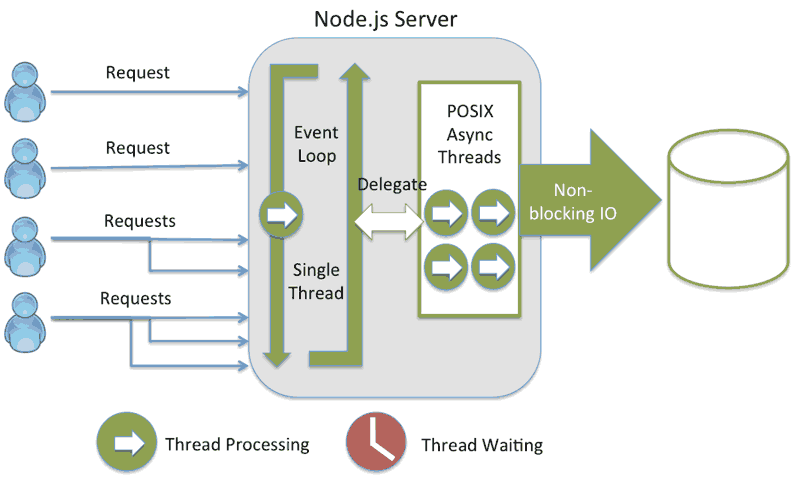
\includegraphics[width=0.9\textwidth]{img/node-js-structure.png}
    \caption{Struttura a single-thread di Node.js per la delegazione di thread asincroni in POSIX}
    \label{fig:async-node}
\end{figure}
 Sotto un punto di vista tecnico, vediamo che l'Event Loop viene gestito dal thread singolo della struttura di Node.js per andare ad inoltrare ogni richiesta ricevuta ad un thread asincrono POSIX che, per la sua natura, crea una procedura non bloccante per la gestione della request. In altre parole, il single thread serve solamente per la gestione degli inoltri di request e di response. 
\newpage
\subsection{Express.js}
Express.js è un framework basato su Node minimalista in grado di poter semplificare l'implementazione di alcune operazioni di base senza nessuna imposizione di vincoli. Questa caratteristica è stata alla base della diffusione di tale framework e dell'implementazione di librerie di terze parti capaci di poter gestire elementi di applicazioni web come cookie, parsing di richieste, gestione degli errori, del login e di gestione di componenti esterne comunicanti. Notiamo che un server in Node.js scritto in Express.js diventa più compatto:
\begin{lstlisting}
var express = require('express');  
var app = express();  
app.get('/', (req,resp)=> {  
  resp.send('Hello World');  
}).listen('8000');
\end{lstlisting}
Nell'esempio sopra riportato, possiamo vedere come si gestisce una richiesta su un URL di radice secondo un'approccio basato su REST in cui si ha la ricezione della request, e l'invio di un messaggio di una response da parte dell'applicazione Express in ascolto sulla porta 8000 in maniera asincrona.
\subsection{Architettura Docker}
Docker è un progetto open source nato con lo scopo di automatizzare la distribuzione di applicazioni sotto forma di contenitori leggeri, portabili e autosufficienti che possono essere eseguiti su cloud (pubblici o privati) o in locale. La tecnologia Docker si basa sul kernel di Linux che garantisce l'isolamento dei processi in modo tale da poter eseguirli in maniera indipendente. Tale caratteristica è alla base delle proprietà del container che riesce ad eseguire una applicazione andandone a rispettare tutte le dipendenze sfruttando l'infrastruttura esistente in modo da poter conservare un buon livello di sicurezza. 
I container Docker consentono il deployment a partire da un'immagine. Ciò semplifica la condivisione di un'applicazione o di un insieme di servizi, con tutte le loro dipendenze, nei vari ambienti. Un'altra caratteristica dei container di Docker è l'automatizzazione della distribuzione delle applicazioni o dei processi che la compongono attuando un meccanismo di replica basato sulla condivisione delle immagini dell'applicazione. Gli strumenti sviluppati partendo dai container Linux, responsabili dell'unicità e della semplicità di utilizzo di Docker, offrono agli utenti accesso alle applicazioni, la capacità di eseguire un deployment rapido, e il controllo sulla distribuzione di nuove versioni.
\begin{figure}[h]
    \centering
    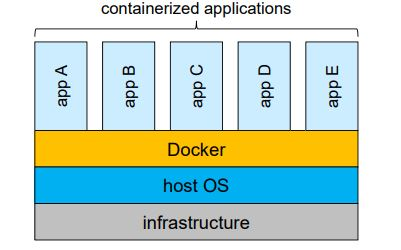
\includegraphics[width=0.9\textwidth]{img/infrastructure-docker.jpg}
    \caption{Struttura dell'architettura Docker}
    \label{fig:infrastructure-dockere}
\end{figure}
I vantaggi nell'utilizzo di Docker sono i seguenti: 
\begin{itemize}
    \item Modularità: la struttura dell'architettura si basa su vari container indipendenti in cui poter gestire varie applicazioni in maniera parallela e autosufficiente.
    \item Sistema di aggiornamento stratificato: Le immagini su cui si basano le applicazioni hanno una struttura stratificata. Ad ogni proprietà alterata dell'immagine, si crea un nuovo strato che andrà ad aggiungersi a quelli pre-esistenti.
    \item Meccanismo di rollback: uno dei maggiori vantaggi della stratificazione è la capacità di eseguire il rollback. Ogni immagine è composta da strati. Se l'iterazione di un'immagine non è soddisfacente, è possibile riportala alla versione precedente.
    \item Facilità di deploy: i container basati su Docker possono ridurre il deployment a pochi secondi. Creando un container per ogni processo, puoi condividere con rapidità i processi simili con le nuove applicazioni. Poiché non è necessario riavviare un sistema operativo per aggiungere o spostare un container, i tempi per il deployment sono sostanzialmente più brevi.
\end{itemize}

\newpage

\voidpage
\chapter{Hyperledger Fabric}
\section{Introduzione}
Fondata dalla Linux Fondation nel 2015 per anticipare le tecnologie blockchain industriali, Hyperledger Fabric si presenta come standard una singola blockchain, incoraggia un approccio collaborativo per sviluppare tecnologie blockchain attraverso un processo di community, con diritti di proprietà intellettuali che incoraggiano uno sviluppo aperto e dinamico.
Hyperledger Fabric è uno dei progetti open-source basato su blockchain all’interno di Hyperledger. Come altre tecnologie blockchain, ha un ledger, utilizza smart contract, ed è un sistema attraverso il quale i partecipanti gestiscono le proprie transazioni.
Dove Hyperledger Fabric si differenzia da altri sistemi blockchain è che è privato e permissioned. Invece che essere un sistema aperto permissionless che permette a identità sconosciute di partecipare alla rete (richiedendo protocolli quali “proof of work” per convalidare le transazioni e rendere sicura la rete), i membri di Hyperledger Fabric sono iscritti tramite un Membership Service Provider (MSP) di fiducia.
Hyperledger Fabric inoltre offre svariate opzioni innestabili. I dati sono immagazzinati secondo una particolare struttura, i meccanismi di consenso possono essere sostituiti, e sono supportati vari MSP.
Hyperledger Fabric inoltre offre la possibilità di creare canali, permettendo a un gruppo di partecipanti di formare un ledger di transazioni separato. Questa è un’opzione particolarmente importante per le reti in cui alcuni partecipanti potrebbero essere concorrenti e non volere che ogni transazione fatta da loro sia nota a tutti i nodi. Due partecipanti formano un canale, questi due, e nessun altro, possiedono le copie del ledger per quel channel preso da riferimento.
\newpage
\section{Funzionalità di Hyperledger Fabric}
Le funzionalità su cui si basa tale progetto sono quelle legate a blockchain di tipo private e permissioned. Le caratteristiche fondamentali che si affacciano verso questo ambiente sono la modularità, la sicurezza, scalabilità e performance. Le funzionalità principali sono le seguenti:
\subsection{Gestione dell'identità}
La gestione delle funzionalità legate a ogni peer è specificato all'interno di un meccanismo di autenticazione proprio delle blockchain permissioned. Vi è un sistema d'identificazione che riesce ad assegnare a ogni utente connesso alla rete un ID univoco. Tale ID specifica i permessi per accedere a particolari funzionalità del chaincode, alla visibilità su alcune strutture dati e sulla distribuzione di un nuovo chaincode.
\subsection{Privacy e riservatezza}
All'interno della gestione della rete su cui si basa Hyperledger Fabric, vi sono meccanismi di privatizzazioni di alcune transazioni, visibili solamente ai nodi collegati a uno specifico canale privato. L'uso di tali canali stabilisce una privatizzazione delle transazioni che permettono di far sussistere più organizzazioni (aziendali o logiche) su una medesima rete. All'interno delle transazioni noi possiamo gestire la riservatezza sia per i dati e sia per informazioni proprie dei membri o del canale. Questo meccanismo garantisce un principio di riservatezza che in altre blockchain sono inesistenti. Inoltre, riesce a sfruttare la sicurezza degli accessi propria delle blockchain di tipo permissioned e private.
\subsection{Processi efficienti}
Hyperledger Fabric assegna i ruoli di rete a secondo delle tipologie di un nodo. Per fornire concorrenza e parallelismo alla rete, si ha una separazione tra le varie operazioni di gestione delle transazioni tra: esecuzione, applicazione e ordinamento. Eseguire le transazioni prima di ordinarle permette a ogni nodo di processarne più di una simultaneamente. Questa esecuzione concorrente aumenta l’efficienza del processo di ogni peer e accelera la consegna delle transazioni al servizio di ordine che operarà successivamente.
Oltre ad abilitare il processo parallelo, la divisione del lavoro libera i nodi ordinanti dalle richieste di esecuzione delle transazioni e di mantenimento del ledger, mentre i peer sono liberati dal superlavoro di ordine che rappresenta l'operazione di consenso per la validazione delle transazioni. Questa biforcazione di ruoli limita anche il processo richiesto per l’autorizzazione e l’autenticazione; tutti i nodi non devono fidarsi di quelli adibiti al consenso e viceversa. In questo modo i processi su particolari peer possono essere eseguiti indipendentemente dalla verifica degli altri avente come risultato quello di separare i ruoli in maniera modulare.
\subsection{Funzionalità del chaincode}
All'interno di Hyperledger Fabric, i chaincode sono utilizzati per definire una logica di business per tipi di transazione propri per un canale, essi specificano la logica per la gestione della strutturazione dei dati e della loro manipolazione. Poichè le transazioni sono proprie di un canale, tutte quelle di una medesima tipologia seguiranno le regole specificate dallo smart contract proprio della sotto-rete (channel). L'altra forma di chaincode ha come scopo principale quello di definire le regole di validazione delle transazioni. 
\subsection{Modularità di Hyperledger Fabric}
Hyperlegder Fabric implementa un’architettura modulare per fornire una scelta funzionale ai progettisti della rete. Algoritmi specifici per l'identificazione, l'ordinamento (definito anche come meccanismo di consenso) e gestione della crittografia, per esempio, possono essere configurati programmaticamente all'interno di ogni rete basata su Fabric. Il risultato è una architettura blockchain universale che ogni industria o dominio pubblico può adottare e personalizzare.
\newpage
\section{Principi su cui si fonda Hyperledger Fabric}
Hyperledger Fabric ha un modello dinamico, incentrato sulla variabilità nella configurazione di alcuni concetti fondamentali che definiscono i punti cardine su cui si appoggi la struttura. Secondo una visione ad alto livello, essi si possono sintetizzare nei seguenti aspetti:
\begin{enumerate}
    \item Privacy: tramite l'utilizzo di collezioni di dati e canali privati, possiamo definire un meccanismo di riservatezza in cui le informazioni di una transazione sono visibili solamente ai soli nodi collegati a un canale. Con tale meccanismo, Hyperledger Fabric soddisfa le richieste di riservatezze dei dati cosi da poter mantenere su una medesima rete più organizzazioni.
    \item Sicurezza: basandosi su una blockchain di tipo permissioned, i nodi che sono all'interno della rete sono autenticati e registrati dentro il MSP (Membership Service Provider). Inoltre, le transazioni sono rilevabili ai soli nodi autorizzati alla visione e alla validazione del loro contenuto.
    \item Consenso: dando dinamicità e flessibilità di gestione all'interno di un unico meccanismo di approvazione e, andando a definirne le caratteristiche in maniera programmatica, si ha un aumento dell'efficienza del sistema di verifica delle transazioni.
\end{enumerate}
\newpage
\section{Componenti funzionali alla base del modello}
All'interno di tale paragrafo andremo a definire una panoramica approfondita delle componenti che vengono utilizzate per il funzionamento di Hyperledger Fabric andando a descrivere le caratteristiche principali per ciascun elemento. Andremo anche a ridefinire alcuni concetti noti all'interno del contesto delle blockchain cosi da poter sottolineare come le funzionalità di tali elementi si adattino al modello offerto da Hyperledger Fabric.
\subsection{Ledger}
Il ledger è una delle componenti principali che si identificano all'interno 
\newline dell'architettura su cui si fonda Hyperledger Fabric. Per definizione, esso non fa altro che mantenere in maniera immutabile una catena d'informazioni inerenti a tutti i passaggi di stati che si sono avuti all'interno della storia della rete su cui si appoggia. In altri termini, mantiene la storia degli stati precedenti e di quella attuale della blockchain. Una transizione di stato si ha quando si invoca un chaincode susseguita dalla creazione e l'esecuzione di una transazione. Vi è un ledger per ogni canale presente sulla rete. Tale ledger è strutturato come una catena di blocchi in cui ogni blocco ha un numero definito di transazioni formate da record con coppie di chiave-valore, inoltre si mantiene uno stato corrente del database in cui sono memorizzati i dati. Poichè il ledger è proprio di un canale e ognuno di essi ha dei membri rappresentati da alcuni peer della rete, per la natura distribuita su cui si fonda Hyperledger Fabric, si ha una distribuzione di una copia del ledger all'interno di ogni nodo che è membro del canale. A ogni transazione, si avrà una transizione di stato che andrà ad aggiornare ogni copia del ledger. Quando si effettua una transazione, si va a operare solamente sulle informazioni contenute all'interno dell'ultimo blocco aggiunto della catena che rappresenta lo stato globale corrente. Tale stato mantiene tutti in valori dei dati che sono visibili a un canale e, di conseguenza, a ciascuno dei suoi membri. Per manipolare lo stato e i dati correnti annessi, Hyperledger Fabric si appoggia su un database che mantiene tutte le informazioni manipolabili. All'interno di tale database sono presenti solamente i dati dello stato corrente e non quelli della storia passata in modo da garantire l'immutabilità propria della blockchain. Il tipo di un database di stato segue una delle seguenti opzioni di 
\newline
\begin{itemize}
    \item LevelDB: rappresenta il database di stato per default, vi sono tante copie distribuite tra i vari membri del canale. I dati sono mantenuti come una sequenza di coppie chiave-valore.
    \item CouchDB: rappresenta un database di stato alternativo basato su una struttura JSON, tale database riesce ad aumentare l'efficienza tramite l'utilizzo di numerose query sui meta-dati codificati sempre in linguaggio JSON e propri del chaincode di riferimento.
\end{itemize}
La scelta di tale configurazione per la persistenza di uno stato è definita programmaticamente all'interno della configurazione dell'architettura del sistema.
\subsection{Smart Contract e Chaincode}
All'interno di Hyperledger Fabric, i chaincode e i ledger costituiscono il cuore della piattaforma. Il ledger definisce tutta la storia dei stati passati e correnti di un oggetto di business, i chaincode definiscono la business logic eseguibile su di essi per la variazione del loro stato. I chaincode non vengono solamente utilizzati per operazioni di transizione su strutture dati interne al canale in cui si è effettuato il deploy, ma anche per definire caratteristiche a basso livello proprie di Fabric. Prima di definire una transazione, bisogna specificare e caricare uno smart contract in modo da poter precisare dati, concetti e processi. Presi insieme, formano il modello di business su cui si basa la comunicazione tra le parti interessate nel completamento della transazione. Usando una rete blockchain, possiamo definire uno smart contract all'interno di programmi eseguibili in modo da poter operare su degli oggetti di business che verranno utilizzati internamente a una transazione. Hyperledger Fabric utilizza i termini smart contract e chaincode in maniera intercambiabile. In generale, uno smart contract definisce la logica transazionale che controlla il ciclo di vita di un oggetto di business contenuto all'interno dello stato globale della rete. Configurazione:
\newline
\newline
In relazione al ledger, uno smart contract accede a due sue parti: la blockchain, andando a poter visualizzare tutte le transazioni effettuate all'interno della rete e uno stato globale che mantiene una cache con i valori correnti di tutti i dati globali e degli oggetti di business del network. In relazione allo stato globale, uno smart contract può compiere tre operazioni principali:
\begin{enumerate}
    \item GET: Che prende delle informazioni tramite query all'interno del database in cui sono immagazzinati i valori che costituiscono lo stato globale. 
    \item PUT: Che crea un nuovo oggetto di business andandolo a inserire all'interno dello stato globale del ledger.
    \item DELETE: Che cancella un oggetto di business all'interno dello stato globale del ledger ma non nella sua storia, ossia esso non sarà più presente nello stato corrente ma la blockchain traccerà sempre le transazioni passate effettuate su tale entità, andando a mantenere la caratteristica d'immutabilità propria dei suoi blocchi.
\end{enumerate}
Per effettuare tali operazioni di base, Hyperledger Fabric si avvale dell'uso di specifiche API. Inoltre, esse sono di fondamentale importanza se all'interno del modello di business vi sono procedure che interessano la lettura, scrittura o la cancellazione di dati, che essi siano persistenti o di sessione.
Un altro aspetto legato a ogni chaincode sono le regole di approvazione (endorsement). Esse sono molto importanti perchè definiscono quali organizzazioni devono firmate una transazione generata da un determinato smart contract in modo tale da poterla considerare valida. Ogni transazione sottomessa viene aggiunta al ledger distribuito ma solamente quelle valide andranno ad aggiornare lo stato globale.
\begin{figure}[h]
    \centering
    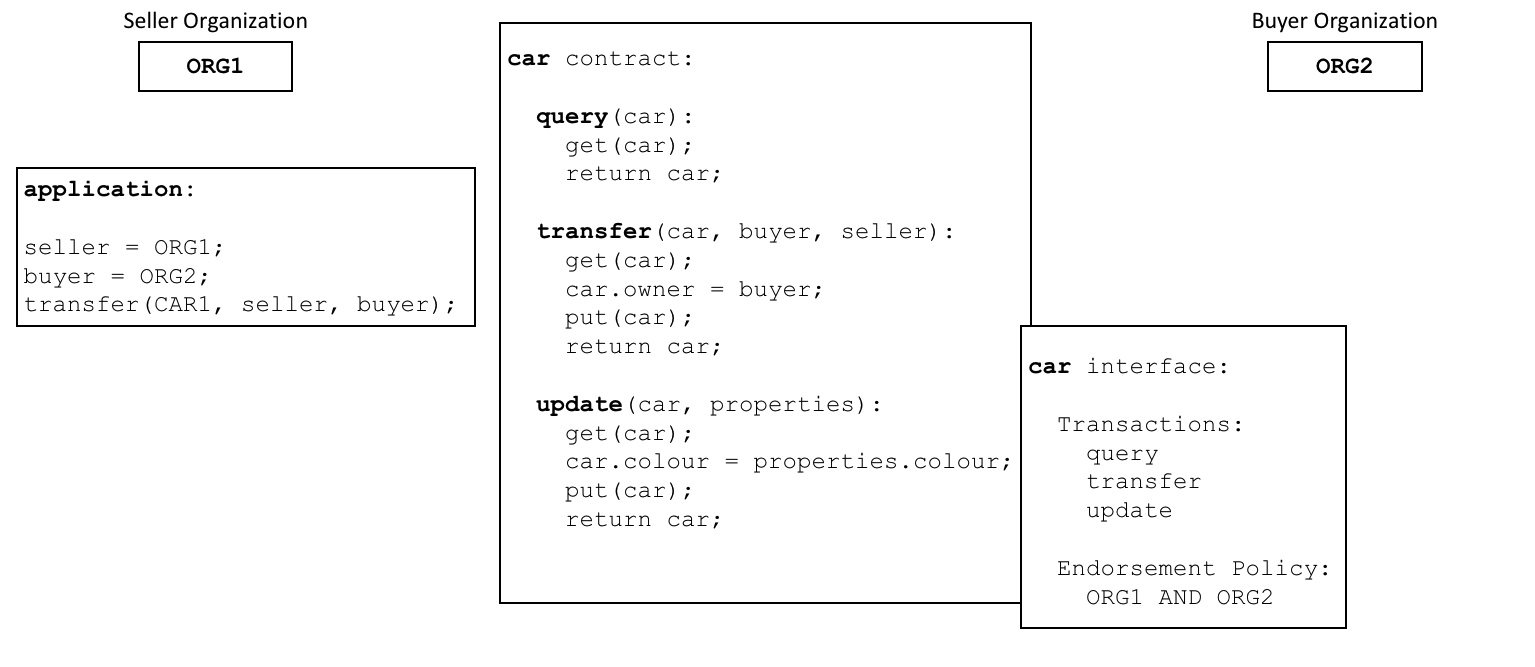
\includegraphics[width=1\textwidth]{img/endorsement.png}
    \caption{Applicazione di un trasferimento di proprietà di un auto}
    \label{fig:endorsement-policy}
\end{figure}
Le regole di endorsement sono una delle caratteristiche che distingue Hyperledger Fabric dalle altre piattaforme legate alle reti di tipo blockchain. Grazie a queste regole, ogni nodo può generare una transazione, ma essa deve essere sempre verificata da specifiche organizzazioni che, rispetto alle classiche blockchain come Bitcoin ed Ethereum, sono definite in un contesto incentrato su una logica che modella più realisticamente il mondo reale. Dato che Hyperledger Fabric si basa su una permissioned blockchain, le regole di approvazione definiscono anche le organizzazioni legate alla validazione delle transazioni, ossia quei nodi che, all'interno della rete, sono considerati affidabili in modo da poter verificare la correttezza delle operazioni eseguite sul network. Le politiche di approvazione sono solamente una delle varie tipologie di regole che si ha all'interno di Fabric, è possibile anche definire dei criteri per la cancellazione e modifiche di dati, oppure per la definizione di quali nodi possono effettuare particolari operazioni di business su specifici oggetti dello stato globale. In tutti i casi, le regole dovrebbero essere concordate all'interno del consorzio delle organizzazioni prima di effettuare una transazione sulla blockchain. In Hyperledger Fabric, ogni tipo di policy può essere programmaticamente modificata rispetto alla forma standard, i meccanismi di aggiornamento delle regole sono anche loro dei criteri di gestione che sono definite all'interno del dominio delle policy della piattaforma. Tramite le politiche di modifica, possiamo anche modificare la logica di endorsement della blockchain su cui si fonda il nostro software. 
Un'altra delle caratteristiche principali sull'utilizzo dei smart contract all'interno del contesto basato su Hyperledger Fabric è il meccanismo di validazione di una transazione mediante l'uso di una proposta transazionale. La procedura di esecuzione di una proposta è eseguita all'interno dell'istanza di un chaincode in un peer dell'organizzazione seguendo le politiche di approvazione proprie del ledger, i valori contenuti all'interno dello stato globale e la logica di business definita nel codice dello smart contract. La risposta alla proposta di transazione è costituita da un set di dati lettura e scrittura, che identificano le informazioni lette dallo stato globale e quelli da scrivere o aggiornare in seguito all'applicazione della transazione. Lo stato globale non viene modificato durante la proposta poiché la transazione deve essere ancora validata. 
\begin{figure}[h]
    \centering
    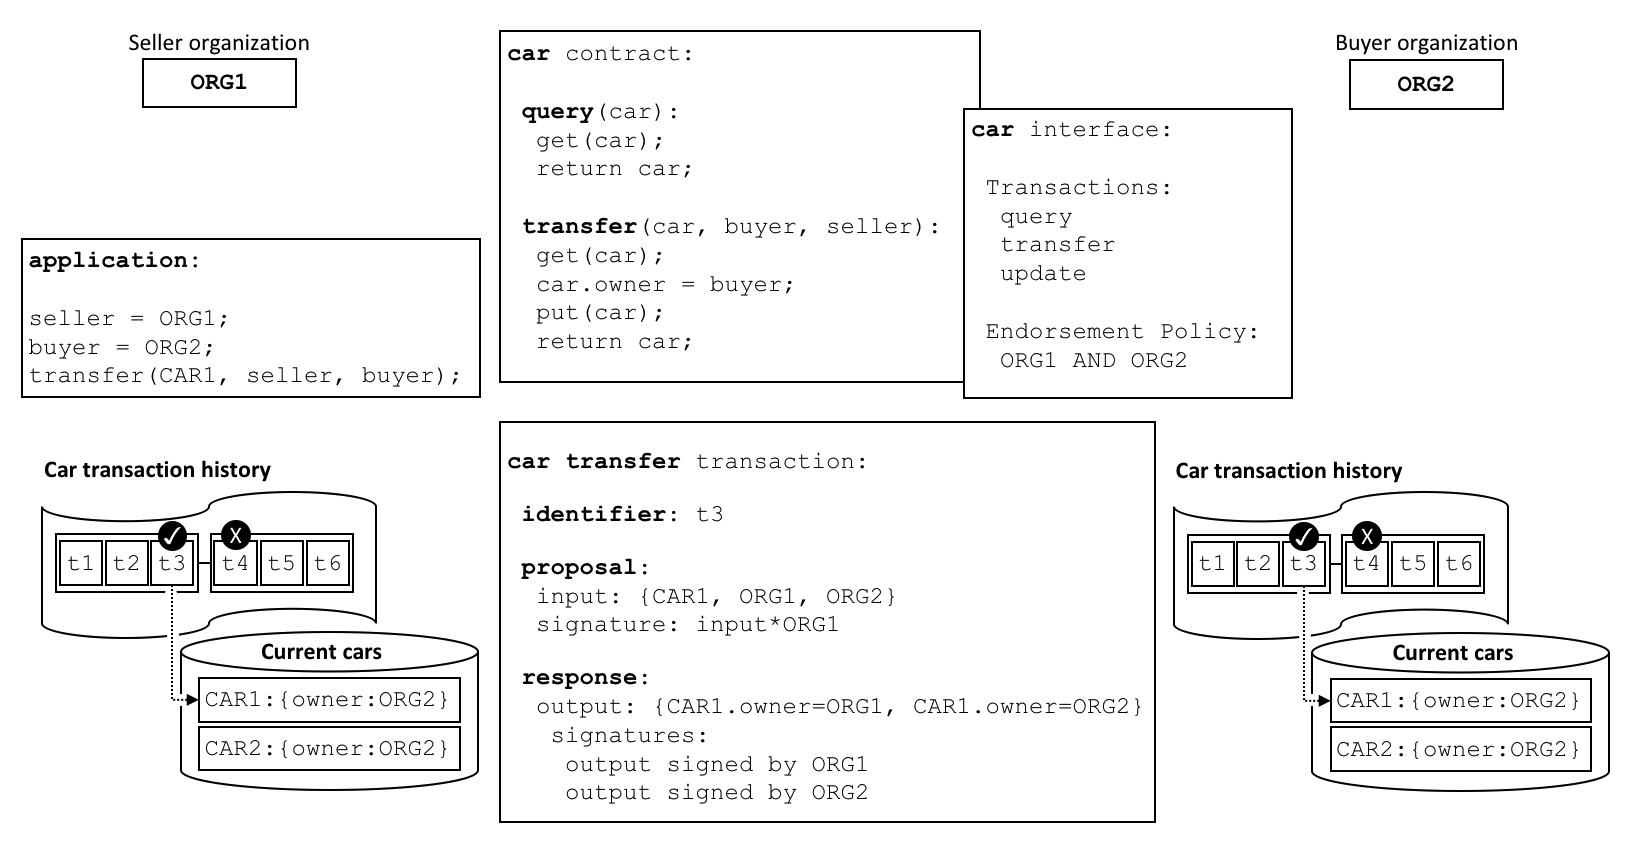
\includegraphics[width=1\textwidth]{img/transaction-proposal.png}
    \caption{Procedimento di una proposta di transazione basata sul caso 3.1}
    \label{fig:transaction-proposal}
\end{figure}
Trovandoci in un ledger distribuito, le transazioni devono essere propagate a tutti i peer di una rete. Prima di ciò, una transazione deve essere sottomessa a due fasi di convalida:
\newpage
\begin{enumerate}
    \item La prima fase si assicura che la transazione è stata verificata con successo dalle organizzazioni specificate all'interno della politica di approvazione legata allo smart contract. 
    \item La seconda fase verifica che lo stato globale corrente sia uguale a quello visualizzato dai peer di convalida nella fase di validazione della transazione, cosi da evitare di modificare i dati nel caso si sono effettuati degli aggiornamenti intermedi.
\end{enumerate}
Se la transazione sotto esame supera queste due fasi di verifica, viene contrassegnata come valida andando a modificare sia lo stato globale e sia la storia della blockchain. In caso non si soddisfi una delle due fasi, la transazione non andrà a modificare i valori dello stato globale ma verrà comunque annessa alla storia della blockchain.
\begin{figure}[h]
    \centering
    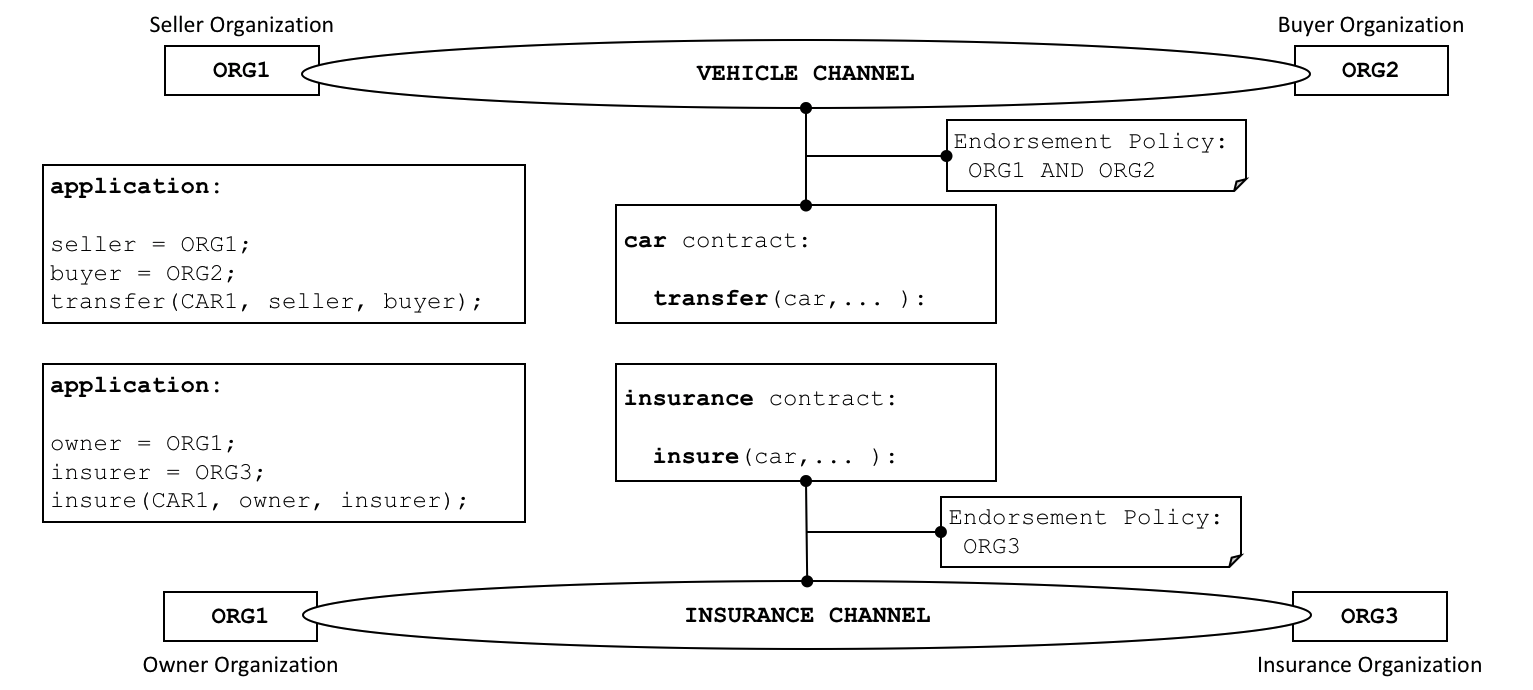
\includegraphics[width=1\textwidth]{img/channel-transaction.png}
    \caption{Architettura di esempio con canali annessi}
    \label{fig:channel-transaction}
\end{figure}
Hyperledger Fabric ha la capacità di poter stabilire più canali indipendenti cosi da riuscire a dividere collezioni e processi di una medesima organizzazione in relazione a controparti differenti e, allo stesso tempo, poter coordinarne le attività dipendenti. Ogni canale dispone di un proprio smart contract che ne definisce la struttura delle transazioni andando a definirne dati, operazioni logiche e parti interessate. A ogni smart contract si ha una politica di approvazione differente e dipendente unicamente dal canale e dai suoi partecipanti. Strutturati in questo modo, i canali rappresentano una propria blockchain. Una medesima organizzazione può essere partecipe in più blockchain senza nessuna restrizione. 
Gli smart contract vengono utilizzati in Fabric anche per la gestione di funzionalità a basso livello indipendenti dai processi aziendali delle organizzazioni presenti sulla rete.
Questi smart contract vengono definiti come chaincode di sistema, e possono essere di uno dei seguenti tipi:
\begin{enumerate}
    \item Lifecyrcle  System Chaincode (LSSC): definisce uno smart contract che gestisce la firma del pacchetto, l'installazione, la creazione di istanze e l'aggiornarnamento delle richieste di un chaincode. 
    \item Configuration System Chaincode (CSCC): istanziato su ogni peer, definisce i meccanismi di gestione e di aggiornamento dei criteri propri di un canale. 
    \item Query System Chaincode (QSCC): Definisce delle query che andranno a comporre le API del ledger per definire delle operazioni su singole transazioni o su interi blocchi della blockchain.
    \item Validation System Chaincode (VSCC): definisce la politica di approvazione, i criteri di strutturazione del set di lettura e scrittura per la verifica dello stato in fase di convalida e le organizzazioni interessate alla validazione di una transazione. 
    \item Endorsement System Chaincode (ESCC): fornisce un supporto ai peer per le firme crittografiche su una transazione.  
\end{enumerate}
Le modifiche ai chaincode di sistema è un processo molto delicato e vulnerabile ai cambiamenti. Essendo una attività molto specifica, un'implementazione scorretta può portare a delle malfunzionalità di alcuni peer come, ad esempio, il voler aggiornare un Validation System Chaincode in maniera differente in più peer di una medesima organizzazione andandone ad alterare il meccanismo del consenso della blockchain sottostante creando eventi come il forking.
\subsection{Peer}
I peer sono le fondamenta di una rete di tipo blockchain. Rappresentano l'unità computazionale capace di poter eseguire processi in maniera distribuita all'interno di una rete. Ogni peer ha una propria copia del ledger e una medesima istanza di un chaincode. Hanno un ciclo di vita indipendente da quello della rete. Possono essere facilmente creati, eseguiti, messi in pausa, riconfigurati oppure cancellati tramite apposite APIs proprie degli amministratori del sistema.
\begin{figure}[h]
    \centering
    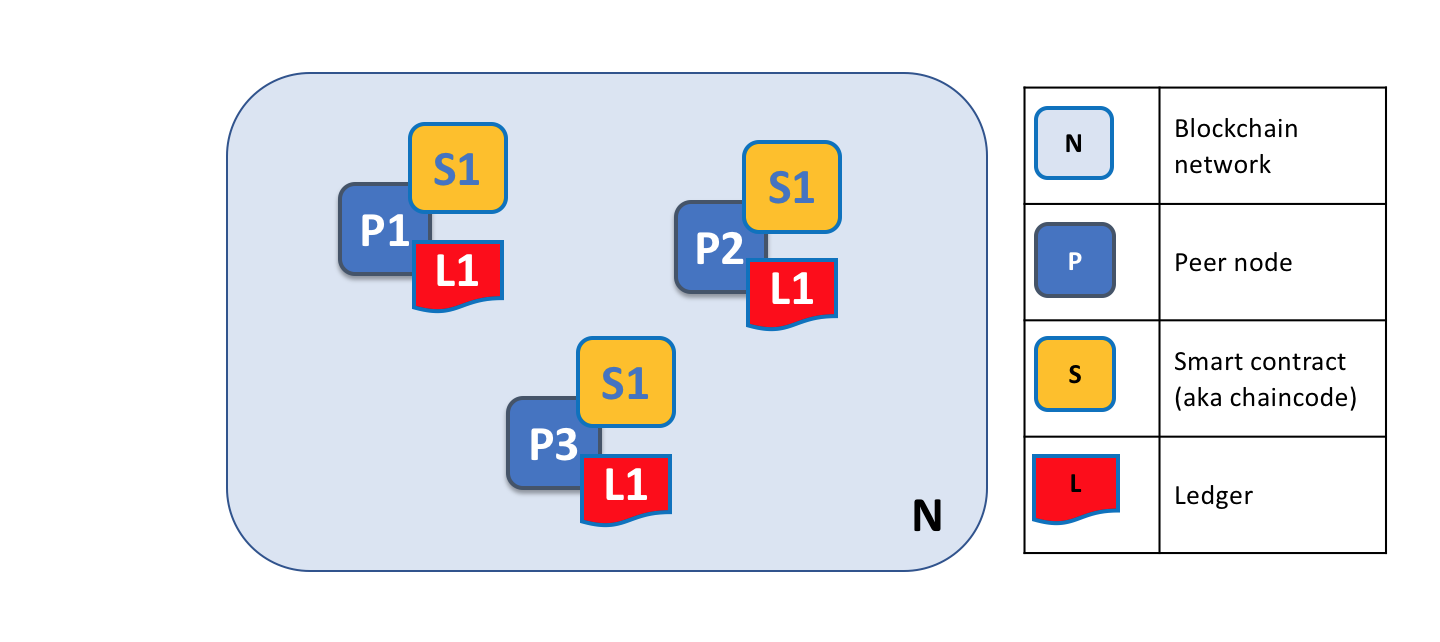
\includegraphics[width=1\textwidth]{img/peer-diagram.png}
    \caption{Visione logica dei peer}
    \label{fig:peer-diagram}
\end{figure}
Notiamo che all'interno di un peer non vi sono chaincode e ledger ma istanze di quest'ultime. Tale caratteristica può prevedere, quindi, che all'interno di un singolo peer vi siano più istanze di chaincode e di ledger. Questo meccanismo offre la possibilità di avere ridondanza che è uno dei principi su cui si fondano i sistemi distribuiti andando ad aumentare anche l'affidabilità delle funzionalità legate a tali elementi. Poichè i peer sono degli host in cui sono localizzate ed eseguite componenti come ledger e chaincode, per poter accedere a questi elementi, bisogna entrare prima al peer che ospita tali istanze. In genere è possibile avere anche istanze differenti di ledger su un medesimo peer, questo garantisce l'interoperabilità tra più ledger distribuiti. Per poter interagire con le istanze dei ledger di un peer, su di esso vanno installati anche i chaincode di riferimento. Tali istanze possono essere assenti anche se configurazioni di questo tipo non sono presenti nei sistemi moderni; questo perchè senza un chaincode di riferimento, il peer non può interagire con il ledger.Notiamo che anche se non vi sono istanze di chaincode per determinare il modello di business su un particolare ledger, all'interno di un peer, per default, vengono sempre installati dei chaincode di sistema per la gestione a basso livello delle funzionalità principali note per la blockchain.
I peer sono dei componenti propri della rete blockchain su cui si fonda Hyperledger Fabric. Tali elementi possono interagire con applicazioni esterne in modo da poter funzionare da mezzo per la gestione delle transazioni sulla blockchain sottostante. La gestione dei peer in relazione alle applicazioni esterne è configurabile programmaticamente tramite l'utilizzo di un SDK dedicato per Hyperledger Fabric. Tramite tale SDK, è possibile gestire i peer e gli altri delle componenti della blockchain tramite l'utilizzo d'interfacce funzionali dedicate. L'interazione tra i peer e le applicazioni esterne non è molto complessa. Il meccanismo di comunicazione può essere riassunto nei seguenti punti:
\begin{enumerate}
    \item L'applicazione si connette al peer all'interno della blockchain
    \item Si invoca una proposta di transazione sull'istanza del chaincode localizzata sul peer che richiama l'istanza del chaincode che esegue l'invocazione richiesta dall'applicazione sui dati dello stato globale del ledger e ritorna una risposta alla query sottomessa. 
    \item L'applicazione riceve la risposta della proposta di transazione, se ha esito negativo termina con uno status di errore interno.
    \item L'applicazione sottomette la transazione all'orderer del canale interessato alla transazione.
    \item L'orderer invia la transazione ai peer in blocco. 
    \item Ogni peer che riceve la transazione aggiorna la propria istanza del ledger andando ad inserire il blocco inerente alla transazione che si è stata effettuata cosi da aggiornare anche la blockchain e lo stato globale. 
\end{enumerate}
\begin{figure}[h]
    \centering
    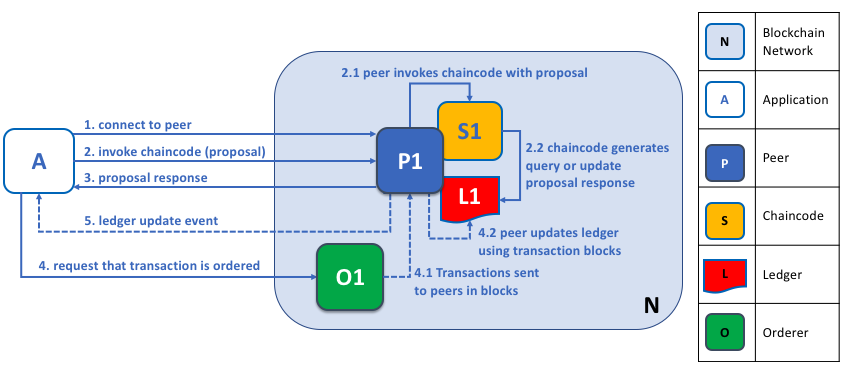
\includegraphics[width=1\textwidth]{img/peer-transaction.png}
    \caption{Transazione sul ledger}
    \label{fig:peer-transaction-process}
\end{figure}
Tutto il procedimento d'invocazione e gestione di una transazione in relazione con un peer, è vista graficamente all'interno della figura 3.5.
Notiamo che una transazione come quella di appena descritta, è propria di tutte quelle operazioni che riguardano l'invocazione di una query all'interno dei dati dello stato globale dell'istanza di un ledger distribuito dentro un peer. La gestione dell'aggiornamento e della manipolazione dei dati distribuiti è data dall'orderer che, come vedremo dopo, è una delle componenti principali per la sottomissione e la manipolazione dei blocchi della catena affiliata a un ledger. Un procedimento simile e più complesso lo si vede, invece, quando al posto di effettuare una query, l'applicazione esterna effettua un aggiornamento dei dati. Questo aggiornamento ha come obiettivo finale quello di andare a effettuare una transizione di stato per qualche oggetto di business del ledger. Tale meccanismo prevede che all'interno dell'aggiornamento del ledger alla fine della sottomissione della transazione, bisogna attendere che tutti i peer di approvazione verifichino la validità della transazione prima di aggiornare effettivamente il ledger, tale politica di acconsenso è verificata con l'uso di ulteriori transazioni che propagano una serie di proposte di aggiornamento a tutti i peer del network. Questa funzionalità è garantita grazie all'impacchettamento delle proposte di aggiornamento in un blocco che viene distribuito a tutti i peer della rete. Se le transazioni di tale blocco vengono verificate dai nodi di approvazione, si passa alla modifica effettiva delle singole copie del ledger all'interno di ciascun peer della rete.
La comunicazione tra i peer avviene per mezzo di un canale. Un canale riesce a mantenere una medesima visione del ledger per un nodo orderer, dei nodi peer e possono interagire anche con applicazioni esterne alla blockchain. La peculiarità principale nell'utilizzo di un canale è data dalla gestione di un medesimo ledger distribuito e per la restrizione della condivisione di dati ai soli peer che sono collegati a tale canale.


\begin{figure}[h]
    \centering
    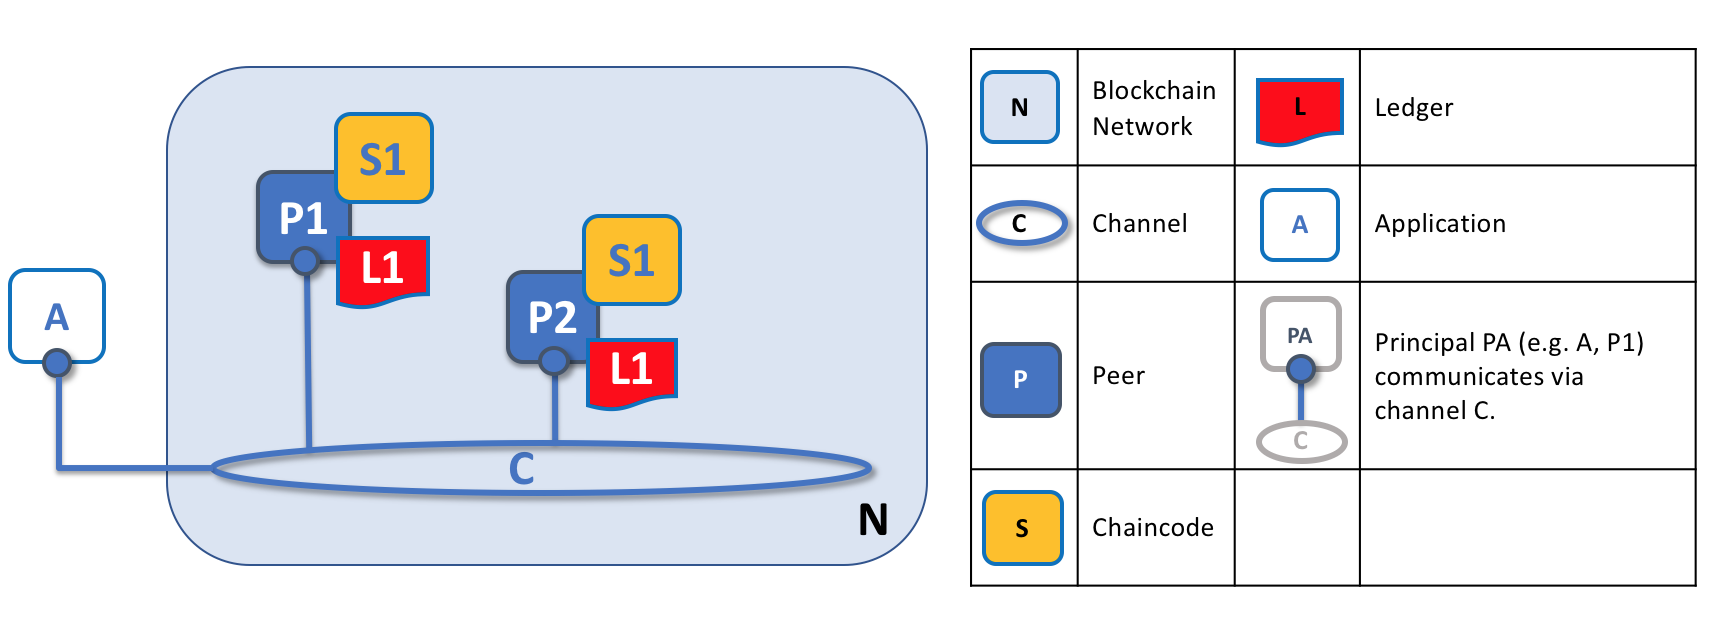
\includegraphics[width=1\textwidth]{img/channel-peer-com.png}
    \caption{Utilizzo di un canale}
    \label{fig:channel-peer-diagram}
\end{figure}
Un altro importante aspetto che riguarda i peer è la loro composizione in gruppi logici chiamati organizzazioni. Le organizzazioni sono un insieme di peer che elaborano delle richieste provenienti, in genere, da una medesima applicazione esterna. I peer che sono propri di un'organizzazione possono anche essere annessi a canali differenti, questo significa che un'organizzazione può collegarsi a più canali e avere visione e gestione di altre transazioni secondo un modello basato sulla privatizzazione delle interazioni e dei dati. Oltre al servizio di ordinamento proprio di un canale, tale struttura non prevede un controllo centralizzato. Anche se tipicamente le applicazioni sono uniche per organizzazione, è possibile avere un'organizzazione che comunichi con più applicazioni che comunicano con molteplici organizzazioni. Questa struttura dinamica è garantita dalla caratteristica della procedura da eseguire: se essa riguarda una query, allora l'applicazione in genere si connette solamente ai peer di una singola organizzazione, se essa, però, aggiorna dei dati, per mantenere il consenso, l'applicazione deve dover comunicare la trasmissione della transazione ai vari peer che hanno il ruolo di validatori secondo le politiche di approvazione del ledger distribuito.
\begin{figure}[h]
    \centering
    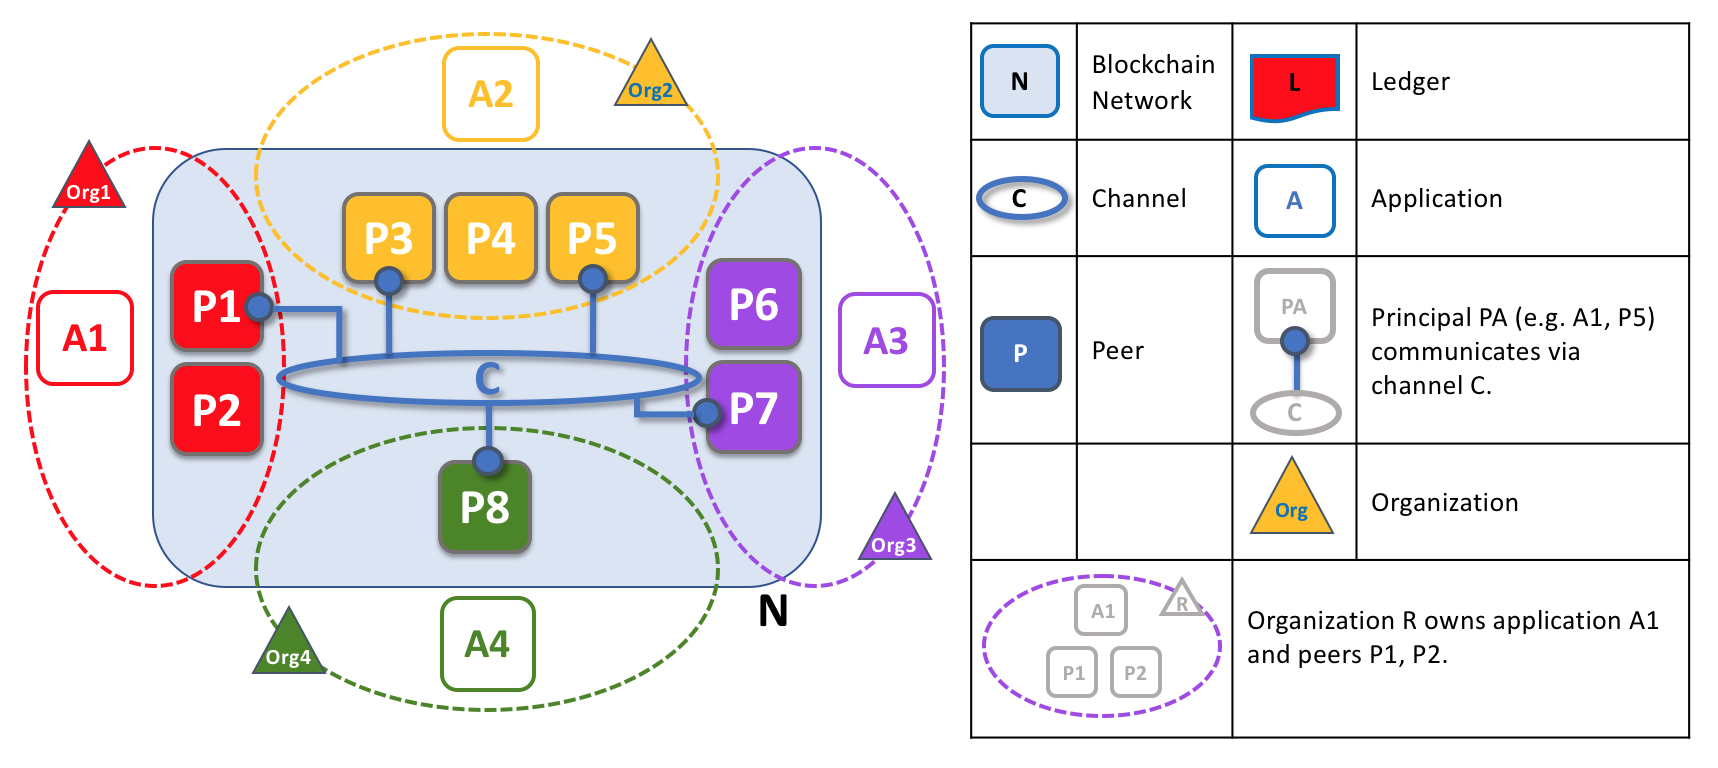
\includegraphics[width=1\textwidth]{img/organization.png}
    \caption{Struttura di una blockchain basata su 4 organizzazioni}
    \label{fig:org-diagram}
\end{figure}
\subsection{Orderer}
Abbiamo visto come i peer possano instanziare ledger e smart contract in modo da poter garantire una interazione con applicazioni esterne mediante lo sviluppo e la gestione di transazioni che vanno a modificare lo stato corrente globale dei dati mantenuti sulla blockchain. Per far si che tutti i peer abbiano la stessa visione dei dati, eseguano le transazioni nello stesso ordine e mantengano uno stato coerente nelle informazioni contenute nella propria istanza del ledger, si ci avvale dell'utilizzo di nodi speciali che vengono definiti come orderer.
Alla base del suo utilizzo vi sono tutte quelle transazioni che vanno ad aggiornare dati del ledger distribuito. Questo perchè se si richiede solamente la lettura dei dati, l'applicazione può co8bmunicare semplicemente con uno dei peer della rete senza dover interpellare altre componenti della blockchain. Invece, quando si tratta di un aggiornamento, si attiva il meccanismo del consenso in cui tutti i peer devono approvare la modifica effettuata e aggiornare i propri ledger. Il procedimento di aggiornamento è molto più lento della procedura che riguarda una semplice query, tale latenza è provocata dalla propagazione della transazione a tutti i peer interessati all'interno della transazione.
Quando si parla di aggiornare un dato all'interno del database di stato del ledger, tutti i peer interessati all'interno della transazione eseguono una procedura di 3 fasi:
\newpage
\begin{enumerate}
    \item Fase di proposta di aggiornamento: un sottoinsieme di peer interessati all'interno della approvazione della transazione, propone una propria versione dell'aggiornamento senza modificare lo stato del proprio ledger.
    \item Fase di impacchettamento: tutte le proposte di aggiornamento vengono impacchettate all'interno di transazioni e inserite all'interno di un blocco. 
    \item Fase di distribuzione e convalida: all'interno di questa fase, l'orderer ha il compito di distribuire a tutti i peer il blocco di transazioni relative all'aggiornamento. Ogni peer andrà a validare le transazioni di tale blocco e, se approvato, verrà aggiornato il ledger distribuito secondo le modifiche delle transazioni proposte. 
\end{enumerate}
Tale procedimento a 3 fasi per l'aggiornamento viene eseguito su blockchain di tipo permissioned. Per altri tipi come Bitcoin ed Ethereum che basano il loro meccanismo di consenso degli aggiornamenti sul Proof of Work, si ha una procedura basata sull'applicazione di un algoritmo di approvazione tipo probabilistico computazionale che, però, sono ancora vulnerabili alla creazione di ledger divergenti tramite forking della blockchain in cui all'interno del proprio ledger vengono accettate le transazioni in ordine differente. In Hyperledger Fabric, invece, tramite l'orderer possiamo ordinare le transazioni e distribuirle per il consenso ai soli peer autorizzati per poi aggiornare tutti i ledger interessati all'interno della blockchain. Tramite l'orderer, l'ordine delle transazioni da accettare è lo stesso e inglobato all'interno di un blocco distribuito cosi da poter eseguire parallelamente l'approvazione su medesime transazioni da parte di più nodi andando ad aumentare l'efficienza e la scalabilità del meccanismo del consenso della blockchain su cui si fonda Fabric. Oltre a organizzare le varie transazioni per la fase di convalida delle transazioni, l'orderer si occupa anche di mantenere traccia di tutte le organizzazioni che hanno i permessi di creazione di un canale. Tali organizzazione formano il consorzio della rete. L'elenco è conservato in un canale di sistema di ordinazione modificabile solamente dall'amministratore dell'orderer. Gli orderer hanno anche il ruolo di amministratori delle operazioni di base che possono compiere i peer delle organizzazioni collegate a un canale andandone a configurare i permessi di accesso, lettura e scrittura ai valori degli oggetti dello stato globale del ledger distribuito. Tali permessi vengono gestiti in fase di convalida di una transazione di aggiornamento proposta da un peer: l'orderer verifica che l'aggiornamento soddisfi i permessi concessi dal peer che ha richiesto la transazione; se approvata, la transazione viene propagata dall'orderer agli altri peer del canale per poi verificare se la transazione soddisfi effettivamente anche le politiche di gestione del canale.
\subsection{Membership Service Provider}
Essendo Fabric una rete blockchain di tipo permissioned, bisogna specificare un meccanismo d'identificazione in modo tale che i peer vengano resi noti in maniera univoca a tutte le altre componenti della rete. Tale meccanismo si raggiunge tramite una procedura basata sull'utilizzo e la distribuzione di chiavi pubbliche all'interno di una blockchain fondata su un meccanismo di fiducia. Le autorità d'identificazione rilasciano in fase di registrazione di un nodo una chiave pubblica, visibile a tutti i peers, e una chiave privata, mantenuta e visibile solamente dal peer proprietario. Poichè la chiave privata non è visibile agli altri peer, si utilizza il Membership Service Provider (MSP) per verificare l'identità di un qualsiasi peer della blockchain. Un esempio della gestione dell'identificazione mediante l'utilizzo del MSP lo si ha nella validazione della firma digitale di una transazione. Quando un peer effettua una transazione, questa viene firmata dal suo creatore mediante la chiave privata, per verificare la validità di tale transazione, ossia che la firma digitale sia effettivamente quella del peer creatore, all'interno del Membership Service Provider viene mantenuto un elenco di tutte le chiavi pubbliche dei peer identificati all'interno della rete.  Notiamo che l'approvazione della transazione ha un alto grado di affidabilità dato che la corrispondenza tra una chiave pubblica e la sua controparte privata è univoca. Il compito di un MSP non si limita a definire solamente l'identità di un peer, ma anche i permessi che ha su un canale a cui è associato definendo cosi anche un ruolo logico rispetto alle operazioni autorizzate che può effettuare. Tale meccanismo è alla base della gestione logica dei dati di Fabric, poiché tramite un MSP è possibile definire i ruoli per singoli peer, organizzazioni o canali. Un MSP definisce i criteri per poter partecipare a una rete autorizzata; essi si concentrano sul soddisfacimento di tali condizioni per i membri della rete:
\newpage
\begin{itemize}
    \item Ottenere una identità da un CA riconosciuto da una rete, ossia acquisire una chiave pubblica e una chiave privata
    \item Far parte ed essere riconosciuto da una organizzazione della blockchain
    \item Aggiungere un MSP al consorzio o al canale
    \item Fare in modo che il MSP sia incluso all'interno delle policy del sistema
\end{itemize}
Sotto un punto di vista implementativo e meno concettuale, un MSP non fornisce nulla, è rappresentato da un insieme di cartelle e file che fanno parte della configurazione strutturale e logica della rete andando a definire le organizzazioni sia internamente (definendo gli amministratori dell'organizzazione) e sia esternamente (definendo meccanismi di validazione delle transazioni andando a rendere partecipi anche peer di altre organizzazioni). Mentre i Certification Authorities sono delle entità che generano delle identità, i MSP sono delle componenti responsabili della loro gestione andando a mantenere la lista delle chiavi pubbliche collegate a ogni ID e utilizzarle per le validazioni di tutte le transazioni aventi come firma quella del peer con l'ID pari a quello preso sotto analisi. All'interno di un MSP si mantiene anche la lista di tutte le Certification Authorities valide in modo da definire un dominio di fiducia di tutte quelle componenti che possono generare delle identità verificate per i membri della rete. Notiamo che un membro della rete non ha solamente un ID univoco che lo contraddistingue, ma anche un ruolo. Tale valore è mantenuto all'interno di un MSP della rete che ha come scopo quello di definire un dominio di operazioni consentite per una particolare entità della rete riuscendo a manipolarle (aggiungere o rimuovere particolari autorizzazioni per uno specifico membro o di una intera categoria).

\subsubsection{Categorie di MSP}
All'interno di una rete blockchain si distinguono due forme di MSP: locali e di canale. In entrambi i casi si hanno le medesime funzionalità, ossia entrambi i tipi di MSP forniscono delle configurazioni di ruoli per ogni identità contenuta al loro interno. La differenza sostanziale che si ha tra le due categorie è l'ambito di applicazioni dei ruoli che definiscono: 

\begin{itemize}
    \item Gli MSP locali vengono definiti localmente all'interno di ogni nodo (peer o orderer) e per i client. Essi definiscono i ruoli in relazione all'ambito applicativo della singola componente (un esempio è quello di definire gli amministratori per un peer oppure chi può operare sul nodo). Gli MSP locali propri dei client, invece, definiscono l'autenticazione per le transazioni sul canale in cui sono membri oppure impostano un ruolo all'interno del sistema come amministratore di una organizzazione. Uno degli obblighi legati a Fabric è quello di dover definire per ogni nodo della rete un MSP locale che definisce chi amministra tale nodo, quale sia la configurazione interna e quali altri componenti hanno diritti di partecipazione sotto quel livello. Altra caratteristica da dover gestire all'interno di un Membership Service Provider all'interno dello scope locale è l'appartenenza a una specifica organizzazione da parte dei nodi aventi come ruolo quello di peer. Cosi facendo, tramite un MSP locale si definiscono amministratori e peer di una organizzazione. Come i peer, anche i nodi con il ruolo di orderer hanno un MSP locale che definisce l'appartenenza a una organizzazione e il dominio di nodi di cui si fida.
    \item Gli MSP globali definiscono i ruoli all'interno dell'ambiente del canale definendone amministratori e partecipanti. Nello specifico definiscono i membri che contribuiscono alla creazione o alla validazione di una transazione propria del canale. Tali MSP definscono le relazioni che vi sono tra le identità e i ruoli dei membri del canale in relazione all'applicazione delle politiche che vi sono su di esso. All'interno di tale MSP vi è la lista degli MSP delle organizzazioni che interagiscono con il canale preso sotto analisi. Ogni organizzazione che interagisce con un canale deve avere un MSP di canale associato, quindi si ha una relazione uno-a-uno tra le organizzazioni che interagiscono con un canale e gli MSP dedicati. Questo perché all'interno di tali MSP si ha la configurazione di come l'organizzazione interagisce con il canale, come viene amministrate, come e quali membri dell'organizzazione partecipano all'interno delle transazioni create internamente al canale. Altro ruolo che si definisce all'interno della configurazione di un MSP di canale è quella della gestione del servizio di ordinamento poiché è possibile avere più orderer che fanno parte di organizzazioni differenti. Tali orderers devono essere configurati per stabilirne una relazione in grado di specificare i meccanismi di consenso e di fiducia per la gestione delle validazioni sul canale. Infine, la memorizzazione di un MSP con scope di canale viene mantenuto, come quello locale, in maniera sincronizzata su più istanze distribuite tra i vari file system dei nodi che interagiscono all'interno del canale.
\end{itemize}
\begin{figure}[h]
    \centering
    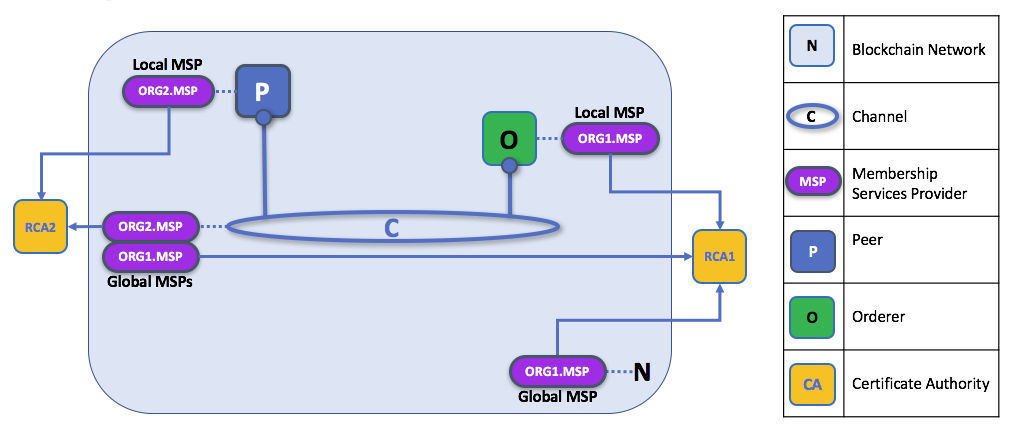
\includegraphics[width=1\textwidth]{img/MSP.png}
    \caption{Architettura di esempio con MSP locali e globali e CA per due organizzazioni}
    \label{fig:msp}
\end{figure}
\newpage
\section{Policy}
Una policy è definita come un insieme di regole che specificano l'infrastruttura per la gestione di un dominio di operazioni eseguite da una particolare o da un gruppo di entità del sistema. In altri termini, definiscono le modalità di accesso, i diritti e come si relazionano delle componenti dell'architettura. Nel caso specifico, le policy su Hyperledger Fabric stabiliscono i criteri di accettazione o di rifiuto di una modifica apportata alla rete, a un canale o a un chaincode. Le policy vengono definite inizialmente dai membri del consorzio, ossia quelle entità in grado di definire la struttura delle componenti di rete (come la creazione di canali). Tale politiche possono essere anche modificate successivamente adottando un approccio evolutivo e dinamico proprio di Hyperledger Fabric.
Le policy è un'altra caratteristica che distingue Fabric da altri tipi di blockchain come Bitcoin ed Ethereum in cui le transazioni possono essere generate e validate da qualsiasi nodo secondo dei criteri fissi con la possibilità di essere modificati solamente in fase d'implementazione andando a modificarne il codice. Hyperledger Fabric, invece, si basa su una blockchain permissioned in cui le policy definiscono la gestione delle transazioni di rete sia in fase compilativa che in quella esecutiva, quali organizzazioni possono accedere e modificare la rete Fabric andandone a specificare anche i metodi applicati, quali organizzazioni possono accedere ad una specifica risorsa come un chaincode di sistema o utente, quali organizzazioni sono interessate per la convalida di una modifica a un canale, di uno smart contract o di una risorsa e i meccanismi di gestione delle firme digitali per la verificabilità di una transazione.
\newpage
\subsection{Tipi di policy in Hyperledger Fabric}
Le politiche di Hyperledger Fabric sono divise secondo un'organizzazione gerarchica differenziando ogni livello per ambiente di utilizzo. 
\begin{figure}[h]
    \centering
    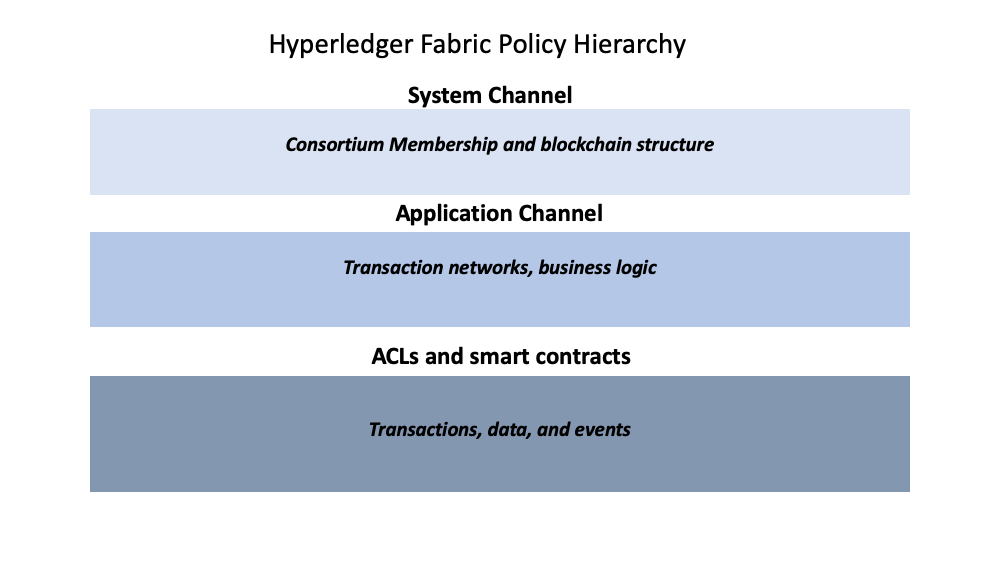
\includegraphics[width=1\textwidth]{img/policy-hierarchy.png}
    \caption{Livelli della gerarchia delle policy in Hyperledger Fabric}
    \label{fig:policy-fabric}
\end{figure}
\paragraph{Configurazione del canale di sistema}
Una delle prime configurazioni prima del caricamento della rete è quella legata al canale di sistema. Tale canale è unico, contiene le organizzazioni legate al servizio di ordinamento e le organizzazioni del consorzio, ossia quelle capaci di effettuare delle transazioni all'interno della rete. Le politiche di configurazione che interessano il canale di sistema regolano il meccanismo del consenso proprio del sistema di ordinamento e la modalità di creazione e di formattazione di un nuovo blocco e, infine, regola anche i membri del consorzio capaci di creare un canale all'interno della rete blockchain.
\paragraph{Configurazione del canale applicativo}
La configurazione di un canale applicativo definisce una comunicazione privata tra alcune organizzazioni del consorzio. Le policy legate a tale configurazioni definiscono la gestione dell'aggiunta o della rimozione di un membro all'interno del canale, definisce anche quali organizzazioni siano necessarie per la validazione dei chaincode prima che questi siano sottomessi definitivamente al commit. Quando un canale viene creato, esso eredita per default tutte le caratteristiche del canale di sistema. I parametri che definiscono la gestione delle operazioni di manipolazione di risorse del canale possono essere personalizzate secondo le regole di configurazione dei canali applicativi.
\paragraph{Configurazione degli ACL e dei smart contract}
La configurazione degli ACL definisce la lista di controllo degli accessi ad una determinata risorsa, ossia quali membri possono accederci. Tramite gli ACL è possibile definire, cosi, la visibilità di una particolare risorsa. Gli amministratori di sistema definiscono la configurazione di tali liste attraverso delle politiche dedicate. Dentro tali regole, è possibile definire l'accessibilità a funzioni di chaincode, a strutture dati oppure ai valori degli oggetti dello stato globale del ledger distribuito. La configurazione di un ACL definisce i criteri di aggiornamento delle risorse proprie di un canale applicativo. Le risorse all'interno delle ACL visibili all'interno della rete su particolari canali applicativi sono mantenuti dentro un file policy specifico chiamato configtx.yaml.
Per quanto riguarda le politiche di gestione del chaincode, esse vengono definite durante la creazione del chaincode stesso e durano per tutto il ciclo di vita del chaincode. Essa può essere definita per default all'interno della configurazione del canale su cui viene caricato, oppure dentro un file specifico che definisce la politica di approvazione del chaincode in cui sono mantenuti i criteri quali la gestione dell'ordinamento e della validazione di una transazione.
\newpage
\section{Dati privati}
Con dati privati andiamo a identificare tutte quelle informazioni che possono essere visibili solamente a un sottoinsieme di account della rete. Nel caso specifico delle blockchain basate su Fabric, tale obiettivo può essere raggiunto andando a definire dei canali dedicati per la visibilità di alcuni tipi di strutture dati. Questa soluzione, però, può causare dei problemi per il sovraccarico dei processi amministrativi della rete (gestione di chaincode multipli, criteri da rispettare, MSP...). Per questo motivo, Hyperledger Fabric dispone di meccanismi in grado di stabilire dei dati privati che sono visibili e gestibili da un sottoinsieme specifico di organizzazioni.
Una collezione di dati è in genere costituita da due elementi:
\newpage
\begin{enumerate}
\item I dati correnti: Mantenuti all'interno di un database di stato corrente distribuito ai vari peer delle organizzazioni autorizzate alla visualizzazione e alla manipolazione di tali strutture mediante l'utilizzo delle istanze dei chaincode proprie di un peer.
\item Un hash dati: In modo da tenere traccia e convalidare le transazioni proprie per quell'insieme di valori e utilizzarle anche per altri scopi legati alla logica di business che si vuole implementare. Notiamo che tale hash ha solamente un riferimento ai dati senza avere nessun collegamento reale.
\end{enumerate}
In seguito riportiamo una figura che rappresenta la differente visione dei dati per un peer di un'organizzazione autorizzata rispetto a un peer di un'altra organizzazione senza diritti di gestione.
\begin{figure}[h]
    \centering
    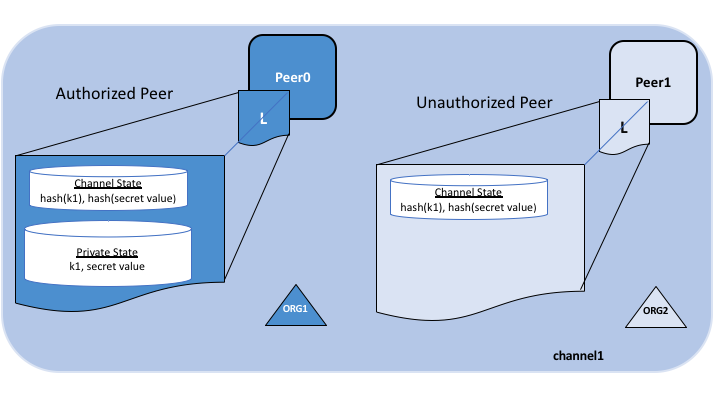
\includegraphics[width=1\textwidth]{img/data-private-vision.png}
    \caption{Gestione della visione dei dati privati}
    \label{fig:private-data}
\end{figure}
I membri della raccolta possono decidere di condividere i dati privati con terze parti, se vogliono trasferire l'asset delle informazioni a nodi esterni al dominio di visibilità dei dati. Le terze parti interessate possono calcolare l'hash dei dati privati e vedere se corrispondano allo stato del libro mastro del canale, cosi dapoter verificarne l'esistenza nel contesto visibile ai membri della collezione.
In molti casi vediamo che le organizzazioni possiedono delle proprie collezioni private che possano essere condivise successivamente a peer di altre organizzazioni tramite la creazione di transazioni che invochino funzionalità del chaincode installato sul canale.
\subsection{Composizione della transazione per i dati privati}
Quando si fa riferimento a raccolte di dati privati dei chaincode, il flusso delle transazioni è leggermente diverso per le proposte, approvazione e l'inserimento nel ledger.
Il flusso di esecuzione che si esegue per tale tipo di transazioni è il seguente:
\begin{enumerate}
    \item L'applicazione client inoltra una richiesta di proposta di transazione per invocare una funzione chaincode (lettura o scrittura di dati privati) per garantire l'approvazione dei peer che fanno parte delle organizzazioni autorizzate della collezione degli asset privati. I dati privati, o i dati utilizzati per generare dati privati in chaincode, vengono inviati in un campo transitorio della proposta di transazione. 
    \item I peer legati alle politiche di approvazione della proposta di transazione eseguono una simulazione della transazione andando a memorizzare lo stato risultante all'interno di registri temporanei e propagano i dati agli altri peer secondo le politiche legate alla configurazione della collezione dei dati privati presa sotto esame. 
    \item I peer di approvazione inviano una risposta al client strutturata come un set di lettura / scrittura andando a mandare l'hash per i riferimenti ai dati privati e i valori risultati reali per i dati pubblici cosi da mantenere un criterio di riservatezza finchè non si è validata la transazione. 
    \item La proposta di transazione verrà rimandata insieme alla transazione effettiva al servizio di ordinamento che includerà gli hash dei dati privati all'interno del blocco di transazione. Tale blocco verrà distribuito a tutti i peer. In questo modo, ogni peer può convalidare il blocco di transazione utilizzando i soli hash di dati privati senza accedere ai loro valori effettivi.
    \item Al momento del commit del blocco, i peer autorizzati utilizzano le politiche di configurazione della collezione per determinare se sono autorizzati ad avere accesso ai dati privati. In caso affermativo, per prima cosa controlleranno il loro archivio di dati transitori locali per determinare se hanno già ricevuto i dati privati durante la proposta di transazione sulle funzionalità richiamate dal chaincode. In caso contrario, tenteranno di estrarre i dati privati da un altro peer autorizzato per poi convalidarli. Al momento della convalida, i dati privati vengono spostati nella loro copia del database in cui è memorizzato lo stato privato della collezione. Infine, una volta terminata la transazione, i dati privati contenuti all'interno dei registri temporanei vengono eliminati. 
\end{enumerate}
\subsection{Politiche di configurazione per i dati privati}
Una delle principali caratteristiche che rappresentano la gestione dei dati privati all'interno di Fabric è rappresentata dai criteri di configurazione delle collezioni privati. In questo contesto, vi si scandiscono alcune proprietà fondamentali capaci di determinare la gestione delle collezioni all'interno dei vari peer della rete in relazione alle richieste di applicazioni client esterne.
La definizione delle collezioni (pubbliche e private), sono mantenute all'interno di un file di configurazione formattato in un array di JSON. Ogni elemento dell'array rappresenta una configurazione della gestione di una struttura dati definita internamente a un chaincode di un canale della rete.
Le proprietà principali delle collezioni sono le seguenti:
\begin{enumerate}
     \item name: Nome della collezione
    \item policy: Rappresentano dei criteri di configurazione della distribuzione delle collezioni private in cui definiscono quali organizzazioni possono accedere ai valori della struttura dati rappresentata dalla collezione. Si utilizza una sintassi basata su una firma OR in cui si definisce tra parentesi le organizzazioni e quali componenti di tali organizzazioni possono effettuare delle operazioni sulla collezione specificata.
    \item requiredPeerCount: Numero di peer delle organizzazioni autorizzate che devono ricevere i dati privati per il processo di convalida della proposta di transazione prima di restituirne una risposta all'applicazione client.
    \item maxPeerCount: Numero di peer massimo tra quelli delle organizzazioni autorizzate per la validazione della proposta di transazione, tale caratteristica è alla base del criterio di ridondanza che mantiene un grado di affidabilità sempre accettabile anche se alcuni peer che sono interessati nel processo di consenso non sono momentaneamente disponibili.
    \item blockToLive: Definisce il numero di blocchi successivi che devono essere creati prima dell'eliminazione dei valori di uno stato mantenuto all'interno di un blocco. Questa proprietà è importante poichè serve ad eliminare blocchi di dati obsoleti. Se si vuole mantenere persistente un blocco in cui è mantenuta una istanza della collezione, tale valore viene impostato a 0.
    \item memberOnlyRead: Se impostata a true, solamente i membri delle organizzazioni dichiarati nelle politiche di distribuzione della collezioni hanno la possibilità di leggere delle informazioni dalla collezione. Nel caso in cui si intenda invocare il chaincode su una funzione di lettura e non si è parte delle organizzazioni a cui si sottopongono questi criteri, l'invocazione ritornerà uno status di errore.
    \item memberOnlyWrite: Se impostato a true, come per la proprietà di memberOnlyRead, definisce una limitazione di scrittura solamente ai membri delle organizzazioni dichiarate nelle politiche di distribuzione della collezione. Quindi l'invocazione di funzioni del chaincode che prevedono un'operazione di scrittura, torneranno un errore se i membri che invocano tale operazioni fanno parte di una organizzazione non autorizzata.
    \item endorsementPolicy: Stabilisce dei criteri che vanno a sovrascrivere quelli del canale in cui è installato il chaincode di riferimento. In questo caso è possibile stabilire un insieme di organizzazione per il consenso e la convalida delle proposte di transazioni differenti rispetto a quelle stabilisce dal canale.
\end{enumerate}
\newpage
\voidpage
\chapter{Progettazione}
All'interno di questo capitolo andremo a discutere dei vari progetti svolti nella fase di tirocinio presso Ericsson Telecommunication con sede a Pagani per un periodo che intercorre tra Maggio a Dicembre del 2019 andandoci a soffermare sui contributi individuali. Ericsson Telecommunication ha istanziato dei fondi per poter produrre progetti sperimentali basati su nuove tecnologie in campo ICT e, nello specifico, nell'utilizzo delle reti che verranno adattate alla generazione 5G. Questo capitolo si baserà sulla progettazione dei vari casi d'uso dei prototipi applicativi basati sulla gestione di una rete secondo il modello basato su blockchain e, nello specifico, con l'utilizzo dell'infrastruttura permissioned fornita da Hyperledger Fabric. L'implementazione inerente a tali progetti verrà discussa nel capitolo successivo. I vari casi sviluppati hanno varie caratteristiche comuni che non hanno subito modifiche in fase implementativa dovuti alla flessibilità di Hyperledger Fabric e la sua adattabilità in vari contesti differenti. Ci siamo occupati di due casi d'uso principali:
\begin{enumerate}
    \item Healthcare: Basato su applicazioni in grado di poter gestire dati sanitari propri di un paziente in un contesto sicuro in cui il cliente era in grado di manipolare i permessi di accesso ai suoi dati privati e sensibili in maniera diretta e senza l'ausilio di terze parti. Nello specifico, si è visto come l'architettura abbia un ottimo utilizzo per le proposte di terapie in risposta ad analisi patologiche registrate dentro il sistema da ospedali. Poichè tali dati sono propri di ogni paziente, egli è l'unico in grado di poter rendere visibile tali informazioni a società terze come cliniche private e centri medici che sono le possibili fornitrici di terapie. Nel caso si dia il consenso alla visualizzazione di tali dati, qualsiasi società terza inclusa nel sistema non potrà ricondurre le informazioni che riceve con la persona reale dato che tali dati verranno rappresentati in forma anonima. 
    \item Automotive: Basato su applicazioni in grado di poter simulare la raccolta dati di sensori montati su componenti automobilistiche in cui la visualizzazione dei dati raccolti è gestita in maniera anonima all'interno di dashboard specifiche per componente, accessibili da società di fornitura esterne autorizzate o aziende proprietarie del prodotto. Il caso d'uso verifica anche come Hyperledger Fabric risponde al sovraccarico di lavoro provocato da continui inserimenti e accessi in rete che sviluppano transazioni da annettere in vari blocchi e leggono le informazioni legate allo stato globale del ledger.
\end{enumerate}
\section{Architettura di base}
L'architettura alla base dei vari progetti sviluppati si basa su una struttura in cui si contraddistinguono varie componenti in comunicazione. Ogni componente fornisce o richiede un servizio internamente all'architettura. Ci soffermeremo particolarmente su come le varie componenti si comportano in ambito di sicurezza andandone a definire i livelli per ogni strato dell'architettura.
\begin{figure}[h]
    \centering
    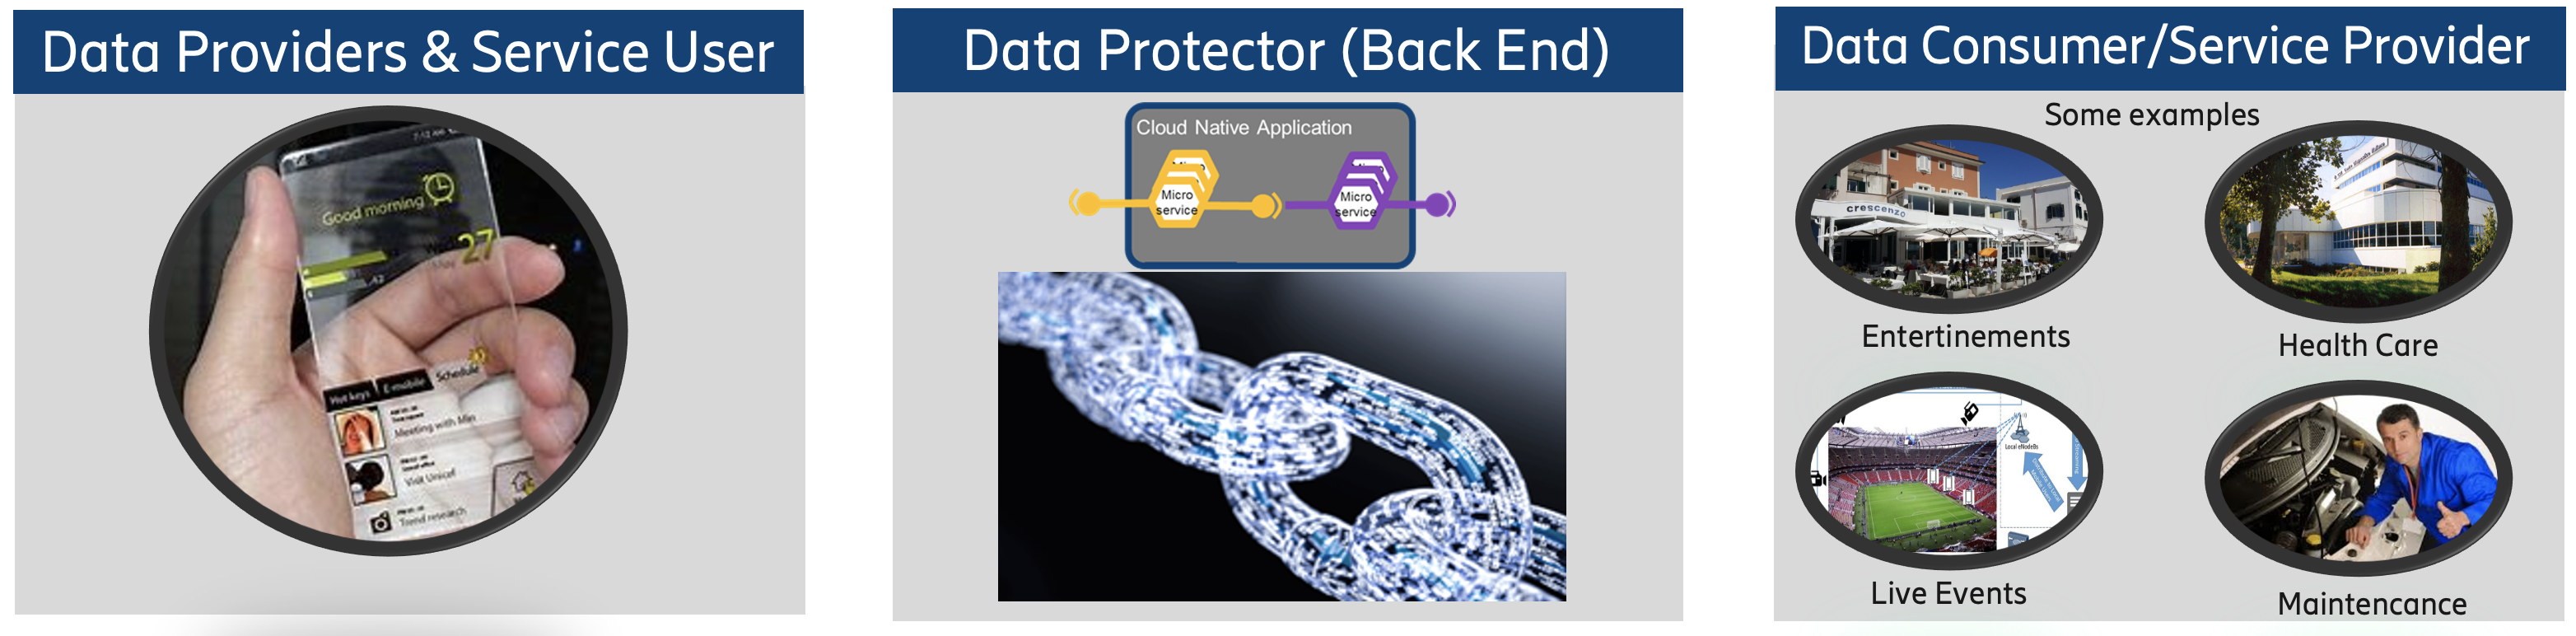
\includegraphics[width=1\textwidth]{img/structure-project-ericsson.png}
    \caption{Gestione della privatizzazione dei dati secondo l'architettura vista ad alto livello}
    \label{fig:architecture-private-diagram}
\end{figure}
\subsection{Progettazione degli strati }
L'architettura del prototipo si basa su una comunicazione che parte da un client (data producer o service provider) rappresentato da un'applicazione mobile o da una interfaccia web in grado di poter richiedereo visualizzare in maniera trasparente i dati con cui si interagisce. Il client comunica direttamente con un server REST appropriato a secondo del tipo di collezione e di operazioni che si intendono manipolare. Ogni server REST avrà, all'interno delle sue funzionalità, tutti i servizi che sono permessi a una specifica organizzazione di peer della blockchain sottostante implementata secondo la struttura logica offerta da Hyperledger Fabric. Il server dispone, quindi, di una serie d'invocazioni a funzioni abilitate per una specifica organizzazione andando a propagare i dati della richiesta del client e inoltrando la risposta fornita dai peer dell'organizzazione che rappresenta. Di seguito andremo a sintetizzare le caratteristiche principali di ogni componente in modo da rappresentare una panoramica generale sul flusso di esecuzione delle attività proposte all'interno del progetto.
\paragraph{Data Consumer e Service Provider}
Ogni client ha delle funzionalità in comune, tali funzioni interessano la gestione delle operazioni di base sulla blockchain della piattaforma che si vuole implementare, esse sono: 
\begin{enumerate}
    \item Registrazione di un nuovo account logico secondo una struttura basata sulla collezione del canale configurato della infrastruttura Fabric sottostante e mantenuta all'interno del ledger andandone a distinguere i vari attori a secondo di una visione fondata sul dominio delle funzionalità della business logic permesse. 
    \item Accesso ai dati dello stato globale del ledger secondo una visione specificata dai permessi di accesso dell'organizzazione. 
    \item Manipolazione dei dati dello stato globale del ledger a secondo dei permessi di visibilità e di accesso dell'organizzazione.
\end{enumerate}
Ciò che distingue i vari client non è solo la visione ad alto livello delle funzioni di cui dispone, ma anche come tali funzionalità sono gestite e visualizzate basandosi su criteri legati alla privatizzazione dei dati.
\paragraph{Server}
I server REST, invece, rispecchiano i servizi invocabili all'interno del chaincode installato all'interno dei canali collegati con i peer dell'organizzazione di riferimento. Lo scopo principale della scelta dell'uso di server di tipo REST è basata sulle proprietà di scalabilità proprie di ogni componente con gestione delle richieste in maniera asincrona. I server rappresentano un ponte che intercorre tra il client e la permissioned blockchain sottostante andando a definire una interfaccia pubblica utilizzabile legata alle invocazioni di funzioni del chaincode del canale Fabric di riferimento.  
\paragraph{Blockchain}
La blockchain rappresenta il contesto persistente di tutta l'architettura, adottandone un nuovo approccio basato sulla decentralizzazione dei dati su uno stato globale di un ledger distribuito e di operazioni di manipolazione o di accesso delle informazioni che generano transazioni mantenute all'interno di blocchi immutabili creati e validati da peer di rete e aggiunti all'interno della catena rappresentata dalla blockchain. 
Sotto un punto di vista logico, la blockchain fornisce contemporaneamente delle invocazioni a funzioni di manipolazione e persistenza dei dati basate su una struttura mantenuta all'interno di un chaincode istanziato dentro ogni peer collegato a un canale della rete e proprio di un canale logico di Hyperledger Fabric. I meccanismi di sicurezza si basano sul sistema di autenticazione basata sulle Certification Authorities e dei Membership Service Provider propri di Hyperledger Fabric cosi da evitare da semplificare il lavoro del programmatore che limita la gestione di questo aspetto solamente sulle possibili configurazioni delle componenti di sicurezza interne alla blockchain. 
\newpage
\section{Applicazione dell'adattabilità dell'architettura }
In seguito ad aver dato una spiegazione generale sulla struttura dell'architettura e su quali casi d'uso si voglia utilizzare, definiamo ora come si è svolto il lavoro progettuale sui due esempi implementati andando a soffermarci sui vari ostacoli che si sono affrontati.
\subsection{Caso d'uso: Healthcare}
La struttura della blockchain inerente a questo caso d'uso si basa sulla gestione di un singolo canale e di due organizzazioni. La prima organizzazione ha i peer che controllato il flusso logico inerente ai pazienti che interagiscono con la base di dati e gli ospedali, la seconda organizzazione, invece, fa riferimento a tutte le cliniche o società sanitarie esterne. Le due organizzazioni si distinguono per l'accessibilità alle collezioni interne al chaincode. Mentre i peer della prima organizzazione possono accedere ai dati pubblici e sensibili, la seconda organizzazione ha i diritti solo per la visibilità delle informazioni pubbliche. 
L'utilizzo di queste due organizzazioni è basata sui collegamenti verso due canali: Un pubblico e l'altro privato. Ogni organizzazione ha un server che definiscono le REST API utilizzabili da applicazioni esterne. Durante la fase di progettazione ad alto livello si sono distinti vari attori, ogni attore rientra in un dominio di permessi che, a sua volta, definisce il dominio delle applicazioni che interagiscono con ciascuna organizzazione. Di seguito riporteremo un'immagine riassuntiva dei ruoli principali che si sono prestabiliti in fase di progettazione: 
\begin{figure}[h]
    \centering
    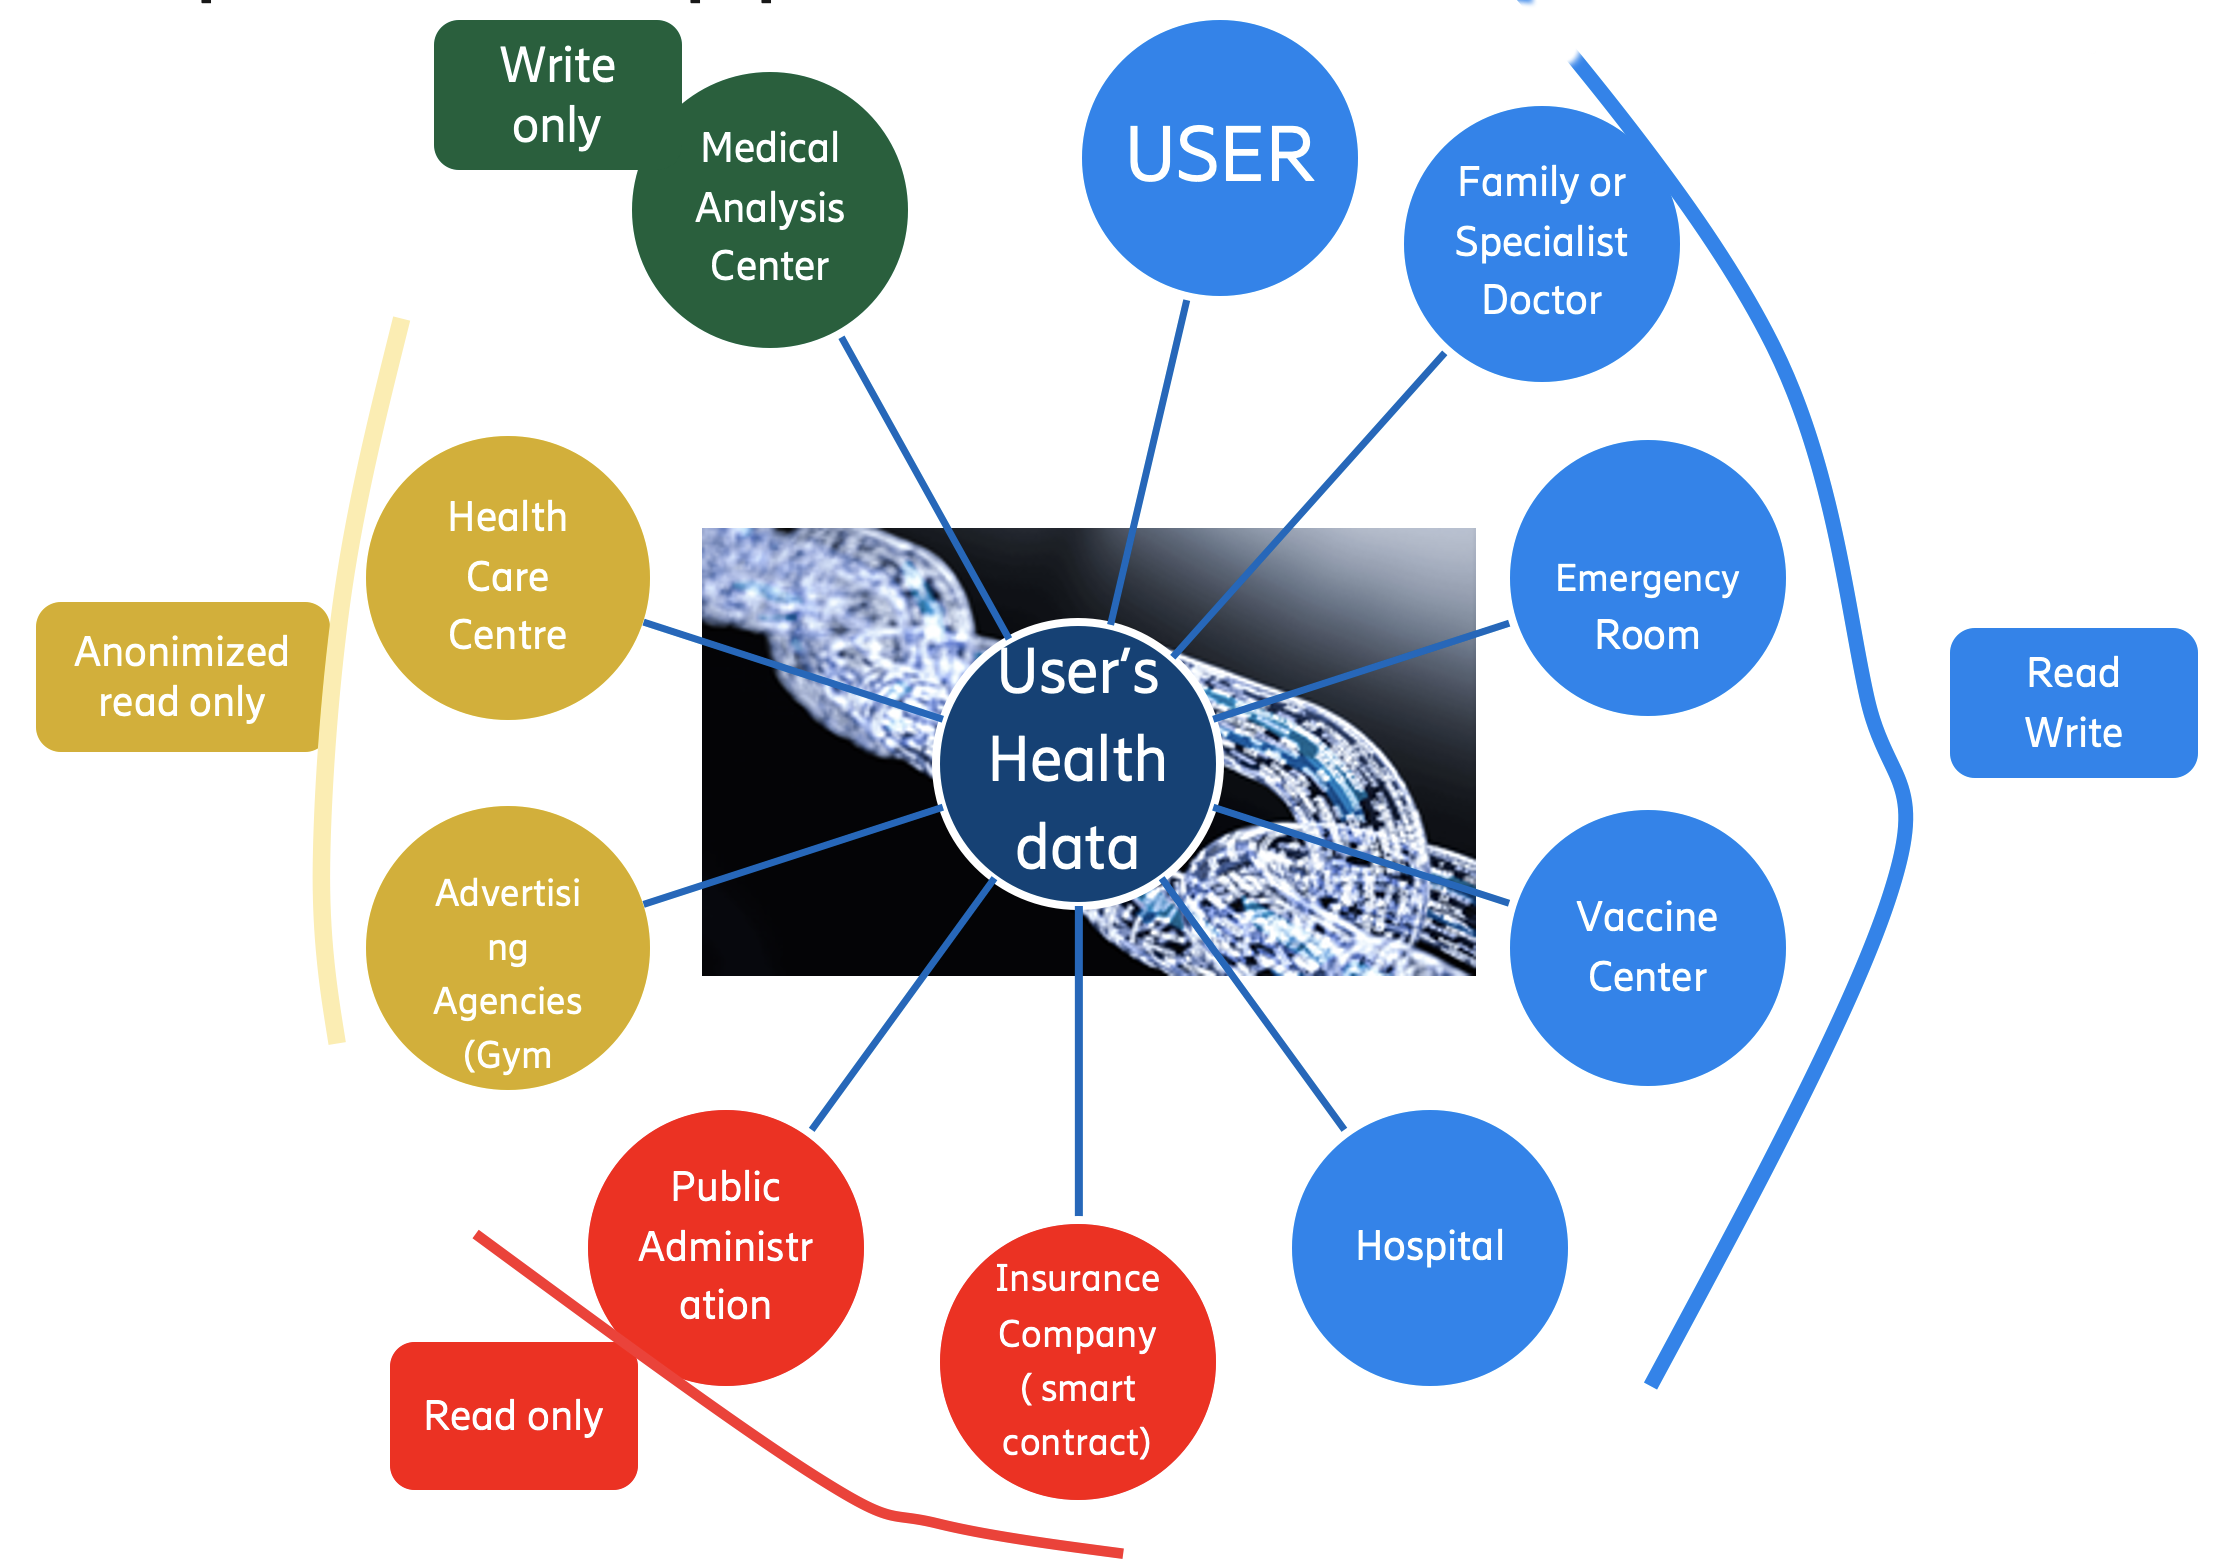
\includegraphics[width=0.6\textwidth]{img/actors-healthcare.png}
    \caption{Dominio progettuale degli attori per un ecosistema sanitario}
    \label{fig:actors-healthcare}
\end{figure}
All'interno della progettazione del prototipo, abbiamo concentrato la progettazione sulla manipolazione dei dati da parte di soli 3 tipi di attori, una per ogni categoria principale:
\begin{enumerate}
    \item User: Il paziente interessato alla gestione dei suoi dati pubblici, privati e sensibile. Ha la massima visibilità sui soli dati personali visualizzabili attraverso l'accesso a un applicazione mobile dedicata in cui poter vedere quali sono le informazioni gestite, andandone a manipolare i permessi e inserirne di nuove. I diritti apportati sono quelli definiti secondo i chaincode dei canali a cui fanno parte i peer della prima organizzazione.
    \item Ospedale: L'ospedale è un attore legato alla lettura e alla scrittura dei dati di ogni paziente ricevuto. Nello specifico, si occupa di leggere informazioni come intolleranze e allergie (dati sensibili) legati a un paziente e scrivere una qualsiasi patologia all'interno della sua cartella clinica decentralizzata e mantenuta dentro il ledger della blockchain. Non vi è nessun meccanismo di anonimizzazione dato che tale entità è autorizzata alla visualizzazione di qualsiasi forma d'informazione legate a una determinata persona sottoposta al processo sanitario. Come per l'utente, ha i permessi di lettura e di scrittura, andando ad accedere alle REST API e ai peer legate alla prima organizzazione.
    \item Centro medico: Il centro medico si occupa di ricevere delle patologie scritte all'interno delle cartelle cliniche di un paziente che ha accettato la condivisione dei suoi dati clinici da parte di società sanitarie esterne. Di seguito alla visualizzazione di queste patologie, è possibile scrivere una cura che verrà visualizzata dal paziente. Tutte le operazioni di scrittura e di lettura su dati visibili al centro medico sono anonimizzati, ciò significa che non sono accessibili i dati inerenti a informazioni personali che possono condurre i dati all'associazione con una persona reale. Tale attore interagisce con il ledger tramite i peer dell'organizzazione due, ciò fa si che accede solamente al canale pubblico senza avere nessuna autorizzazione per il canale privato.
\end{enumerate}
\subsubsection{Contributi individuali}
I contributi individuali sia in fase progettuale che in fase implementativa interessano l'implementazione del centro medico, delle REST API della seconda organizzazione con cui interagiscono i possibili service provider rappresentate da società esterne al sistema sanitario nazionale e dell'adattabilità della blockchain alla struttura desiderata andando a raffinare meccanismi come la configurazione delle policy per la visibilità, dell'accesso e della manipolazione del ledger.
\subsection{Caso d'uso: Automotive}
Altra parantesi si ha con il caso d'uso basato sul contesto dell'Automotive. All'interno della sua progettazione si ha come obiettivo principale quello di definire un sistema di monitoraggio per le componenti di un autovettura proprietaria in cui solamente chi ha i diritti di accesso verso il bene o una sua componente possono seguire in tempo reale le statistiche generate. L'adattabilità dell'architettura si basa sulla gestione di quattro organizzazioni all'interno della blockchain, ognuna legata ad aziende responsabili della fornitura o del possesso del bene. All'interno del prototipo abbiamo distinto tali componenti in freni, gomme, motore per i fornitori andando a lasciare un'organizzazione per l'azienda proprietaria o il proprietario dell'autovettura. Ogni componente è diviso in una collezione privata specifica, ogni organizzazione ha i diritti di visibilità sulla propria componente o, in caso si ci riferisce all'organizzazione proprietaria, su tutte le collezioni. Cosi facendo, i fornitori possono controllare problemi di prestazione su una particolare auto in movimento senza interessarsi delle altre componenti.
La struttura dell'architettura adattata per tale caso d'uso si presenta secondo tali principali componenti:
\paragraph{Client} 
All'interno della progettazione del prototipo, i client di riferimento si dividono in due tipi: 
\begin{itemize}
    \item Client di simulazione: In cui hanno la funzione di aggiornare i dati all'interno dello stato globale del ledger.
    \item Client di visualizzazione: In cui hanno la funzione di leggere i dati dei valori di alcune collezioni contenute all'interno dello stato globale del ledger. 
\end{itemize}
Il client simulatore progettato ha il compito d'inserire, con frequenza costante, dei dati che simulano il comportamento delle componenti su un auto in movimento. Tali aggiornamenti andranno a creare dei blocchi all'interno della blockchain in cui le transazioni conterranno lo stato dei parametri delle componenti in un determinato istante durante la fase di movimento di un auto. I client di visualizzazione che si sono progettati, invece, hanno il compito di leggere lo stato globale nelle sole collezioni in cui hanno autorizzazioni. Tali client si presenteranno come delle dashboard che andranno a visualizzare e confrontare i dati ricevuti graficamente.
\paragraph{Server}
I server sviluppati seguono la stessa logica del caso d'uso Healthcare, in questo caso avremmo quattro server REST che forniscono un'interfaccia pubblica per l'invocazione di funzioni autorizzate all'organizzazione di riferimento.
\paragraph{Blockchain}
La blockchian sottostante distingue i permessi per quattro Membership Service Provider legate alle quattro organizzazioni che elaborano su un medesimo ledger distinguendone la visione secondo i soli permessi andandone a distinguere un canale privato da uno pubblico logico e differente per i peer delle varie organizzazioni.
\subsubsection{Contributi individuali}
All'interno della progettazione del caso d'uso e dell'implementazione del prototipo, ho sviluppato le dashboard, andando ad adattare i server REST all'interfaccia pubblica da e verso le collezioni della blockchain. Inoltre, sono stato il responsabile dell'architettura interna della blockchain andando a definire e configurare i vari peer delle varie organizzazioni andando ad adattare la definizione e l'istanziazione dei chaincode, del ledger e della logica di business del canale tramite le policy di configurazione di Fabric.
\section{Osservazioni finali in fase di progettazione}
All'interno delle conclusioni della fase di progettazione dei protitipi, si vuole fornire un differente fine all'interno dei due casi d'uso. Mentre all'interno del contesto sanitario vogliamo filtrare i dati, andando ad anonimizzare le identità dei pazienti a secondo della tipologia di attore che interagisca con la blockchain, all'interno del secondo caso d'uso, abbiamo anonimizzato i dati a secondo del tipo di attore ma si ha avuto maggior interesse nel vedere come Hyperledger Fabric rispondeva al sovraccarico di lavoro definendo cosi anche i limiti dell'architettura.
\newpage 
\voidpage
\chapter{Implementazione e Risultati}
Andremo ora a soffermarci sull'esperienza diretta avuta sull'approccio alle tecnologie descritte precedentemente nel capitolo due, andando a definire delle implementazioni concrete su casi d'uso descritti nel capitolo quattro. Ci soffermeremo solamente su come le varie componenti comunichino tra di loro con la blockchain alla base dell'architettura. Descriveremo l'implementazione dei vari strati andando a specificare le scelte implementative effettuate nei due casi d'uso concretizzati in fase di progettazione. Concluderemo con la fase di raffinamento dei prototipi in modo da poter rispettare i criteri prefissati in fase progettuale andando a documentare passo dopo passo attraverso i principali snippet di codice che sono alle fondamenta di alcuni concetti funzionali del progetto. Il contesto su cui si concentra questo capitolo è basato solamente sull'implementazione delle componenti sviluppate singolarmente specificate nei contributi individuali all'interno del capitolo quattro.
\section{Client}
Sotto un punto di vista delle applicazioni rappresentanti data consumer o service provider, ci siamo concentrati sull'implementazione dei vari client legati ad alcuni attori andando a concentrarci sulla formattazione dei dati secondo la visione proposta dai server REST definita in back-end. Inoltre, si è aggiunto un ulteriore livello di protezione andando a controllare la formattazione e la correttezza dell'input in modo da evitare di generare delle request non valide, questo approccio di controllo ha lo scopo di allegerire il carico di lavoro del thread in event loop sul server REST.
\subsection{Front-End implementato nel contesto Healthcare}
Nel contesto sanitario, l'implementazione front-end si è concentrato sullo sviluppo dell'interfaccia grafica e sulla rappresentazione dei servizi offerte all'interno delle applicazioni in possesso degli attori principali del prototipo (Paziente, Centro Medico e Ospedale). Si sono sviluppate due applicazioni di tipo mobile, una per il paziente e una per l'ospedale, in cui poter eseguire tutte le funzionalità descritte in fase di progettazione. I miei contributi in questo strato di progettazione si sono concentrati sul centro medico che, invece, dispone di un'implementazione più semplice, basata su un'applicazione web che visualizzava un insieme di dati estrapolati dallo stato globale del ledger. Tali dati sono resi visibili al centro medico mediante i permessi di accesso propri della seconda organizzazione della blockchain. La struttura dell'applicazione front-end ricopre un'interfacciamento verso il server REST attraverso l'utilizzo di Servlet. Le Servlet non fanno altro che stabilire un canale con il server REST, inviare le richieste formattate in JSON e inoltrare le risposte all'interno della sessione dell'applicazione, di seguito riportiamo uno snippet di codice in Java inerente alla creazione della connessione per l'invocazione di un servizio di aggiornamento delle terapie della collezione riferita ai dati sensibili di un paziente sul server REST dedicato alla seconda organizzazione della blockchain:
\begin{figure}[h]
    \centering
    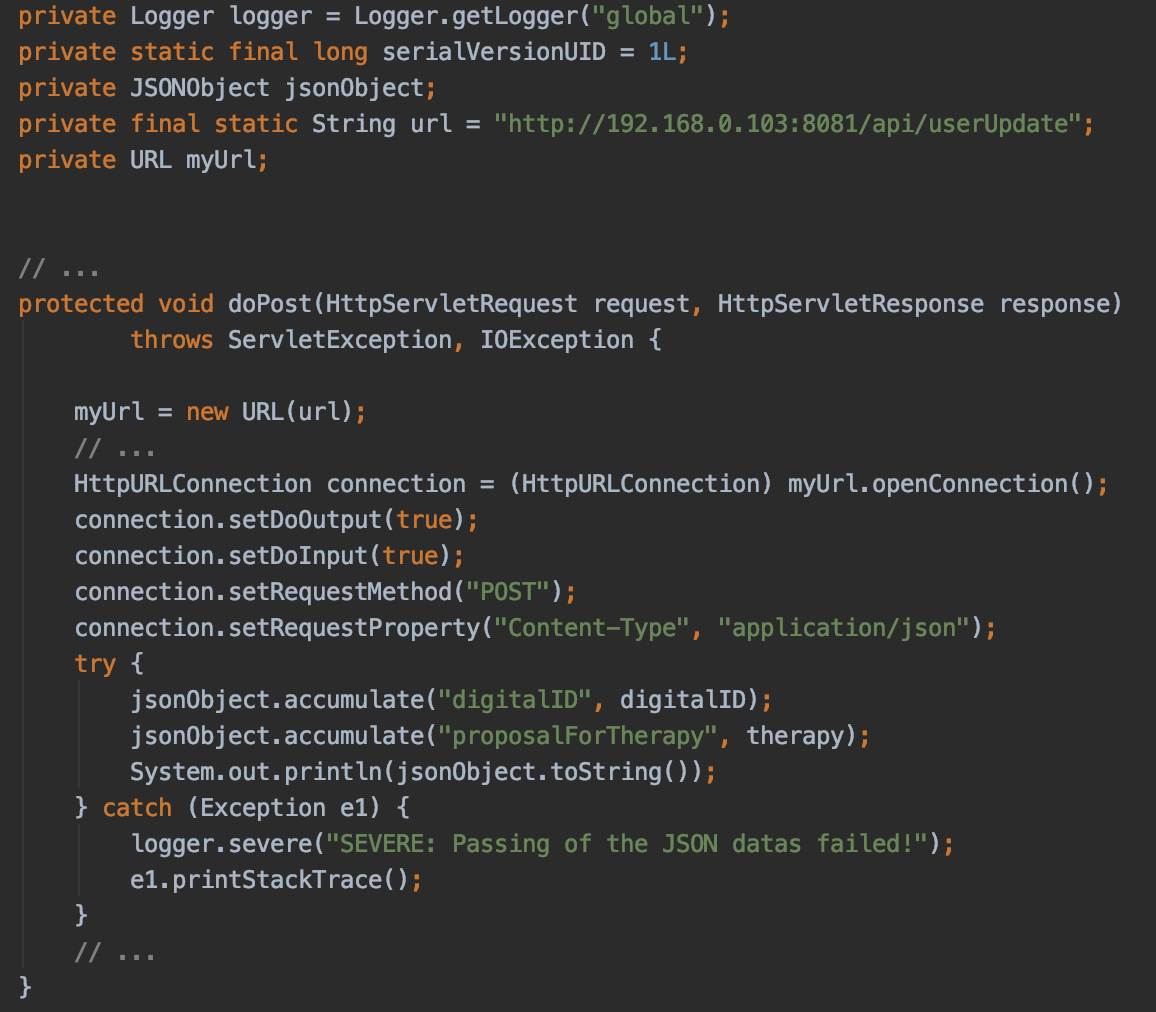
\includegraphics[width=0.6\textwidth]{img/connection_healthcare.png}
    \caption{Approssimazione dell'apertura di una connessione con il server REST all'indirizzo}
    \label{fig:connection_healthcare}
\end{figure}
\newpage
In seguito alla creazione di una connessione, si definisce un oggetto JSON da inviare, nel caso dell'esempio si invia una stringa rappresentante una proposta di terapia per un particolare paziente identificato da un UUID:
\begin{figure}[h]
    \centering
    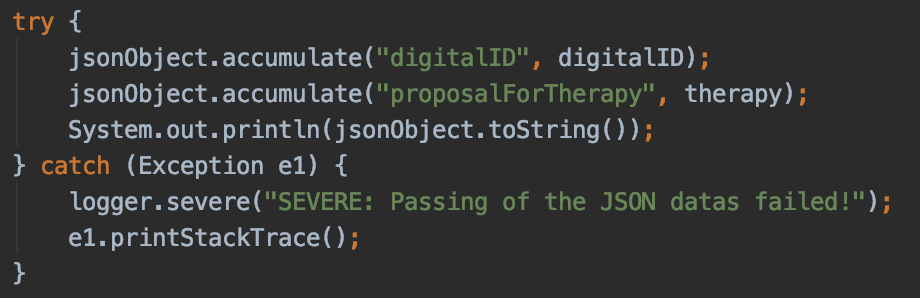
\includegraphics[width=1\textwidth]{img/json_object.png}
    \caption{Costruzione dell'oggetto JSON da inviare ad una request verso un server REST}
    \label{fig:json_request}
\end{figure}
In seguito dell'inoltro della request formattata in JSON, la Servlet attende una risposta dal flusso di input della connessione. Nel caso in esempio, si ha una stringa che rappresenta un array di JSON corrispondente a una serie di entità di una collezione mantenuta all'interno dello stato globale del ledger. La gestione della risposta è simile a come segue:
\begin{figure}[h]
    \centering
    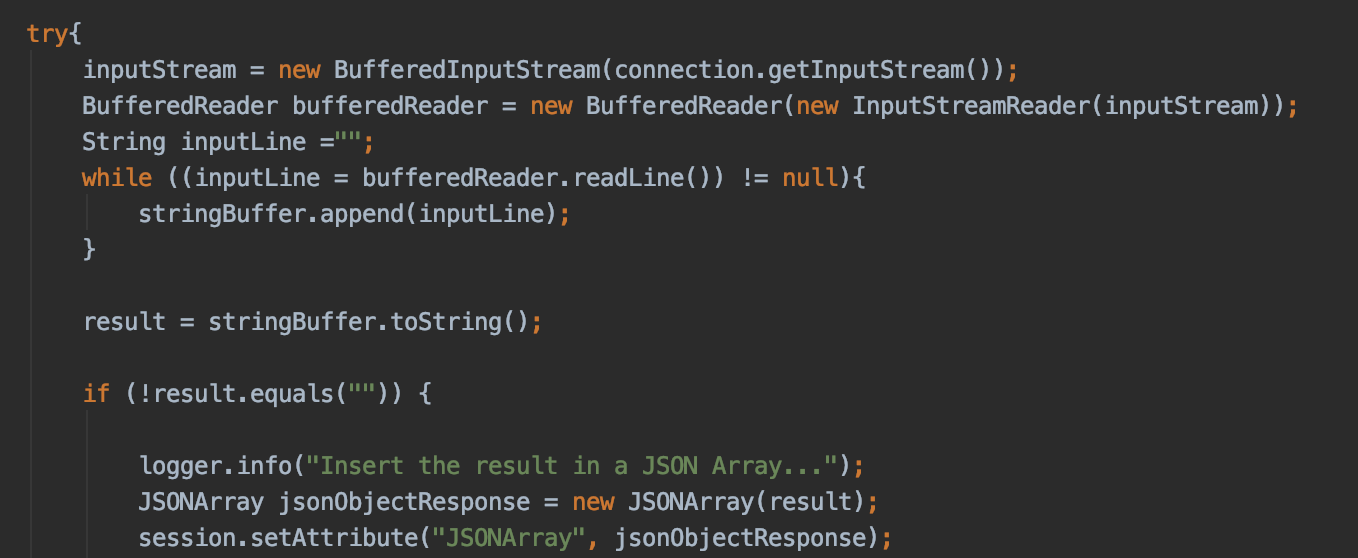
\includegraphics[width=1\textwidth]{img/response_string.png}
    \caption{Formattazione ed inserimento della response della REST API all'interno della sessione del client}
    \label{fig:json_response}
\end{figure}
Nei snippet di codice sopra riportati si può vedere come l'utilità della servlet sia principalmente quella di stabilire un canale di comunicazione con il server andando a formattare in JSON i dati di input e inserire in sessione i dati di output in modo da poter essere visibili e utilizzabili all'interno delle pagine web visualizzate. Per tutte le altre operazioni inerenti alle applicazioni in front-end si ha, come base, quella dell'esempio di modifica riportato in precedenza. 
\subsection{Front-End implementato nel contesto Automotive}
Nel contesto Automotive, il lato front-end comprende un insieme di dashboard e un simulatore di aggiornamento dei dati parametrici sulle collezioni rappresentanti le componenti dell'auto sotto monitoraggio. L'aggiornamento simulato prevede l'inserimento di una serie di valori che andranno ad aggiornare un'entità dello stato globale del ledger creando, a una determinata frequenza, delle transazioni che vengono inserite all'interno di nuovi blocchi collegati alla blockchain. Le dashboard leggono, contemporaneamente, i dati su una singola componente o di tutte le componenti di un'auto a una determinata frequenza. Dentro questo paragrafo andremo ad analizzare solamente un esempio d'implementazione relative alle funzionalità delle dashboard. Ogni dashboard ha una struttura simile, le funzionalità si distinguono principalmente per i tipi di dati che richiedono andando a mantenere una medesima logica funzionale. Possiamo ora analizzare un esempio d'implementazione per la richiesta e il prelievo dei dati andandone a considerare la loro lettura inerenti alle informazioni legate al motore di un'auto identificata tramite un UUID.
\begin{figure}[h]
    \centering
    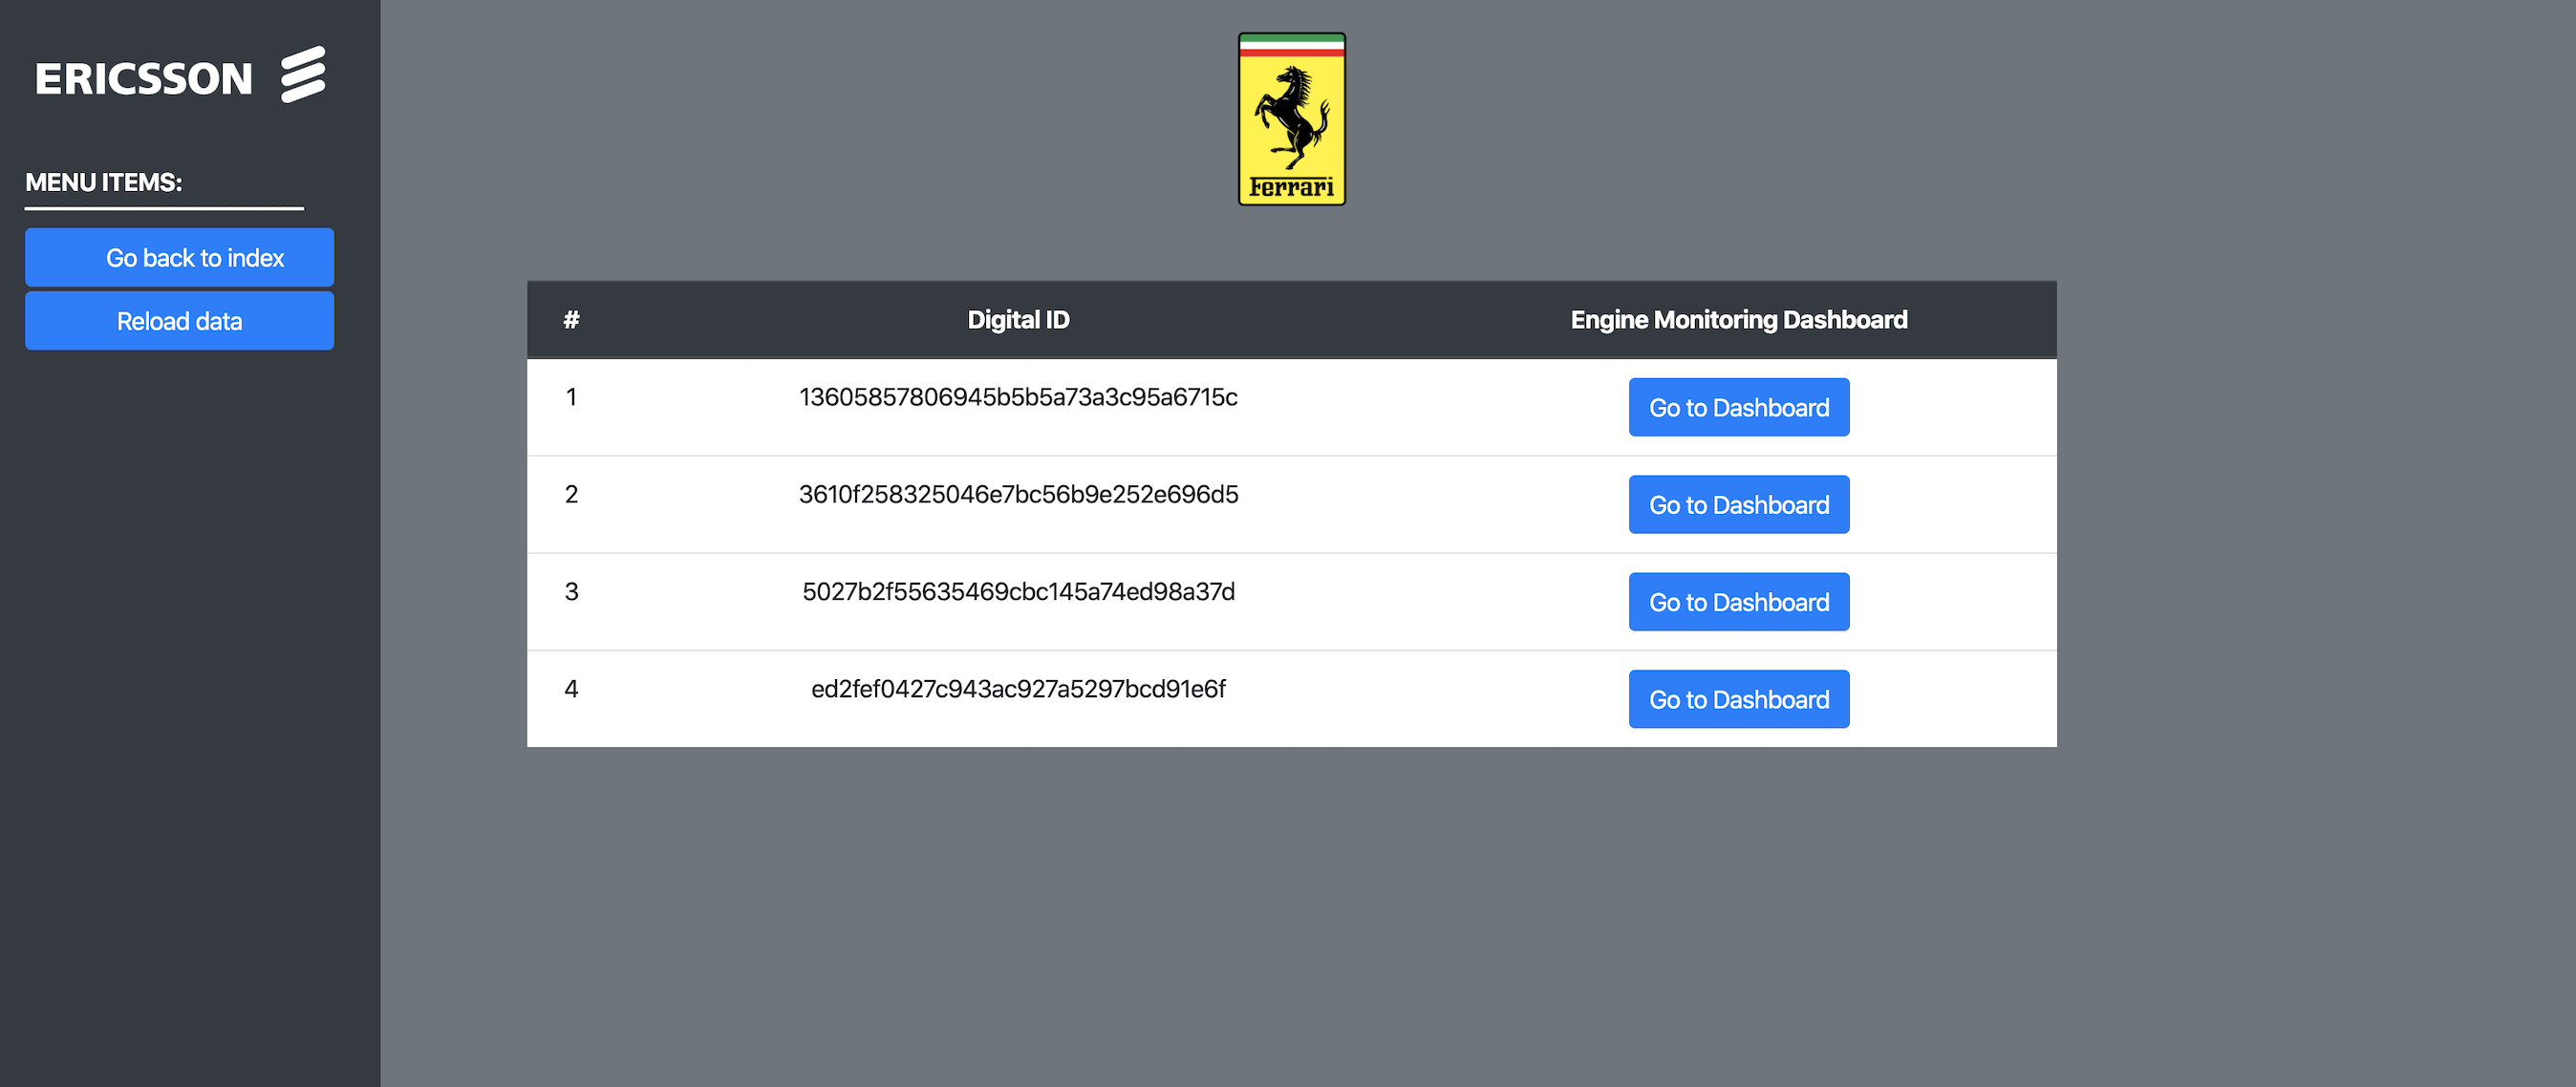
\includegraphics[width=1\textwidth]{img/table_engine_dash.png}
    \caption{Tabelle delle varie entità registrate all'interno dello stato globale della blockchain}
    \label{fig:table_dash}
\end{figure}
La comunicazione con il server REST è assegnata a una Servlet d'interfacciamento che si occupa di gestire i dati di sessione, creare una connessione e formattare le informazioni di input e di output. La logica di business propria della Servlet è simile al caso d'uso sanitario. L'unica differenza si ha per la gestione della sessione che non prevedono l'inserimento di una lista di dati letti dallo stato globale del ledger della blockchain, ma gli stati delle informazioni "storiche" mantenute negli ultimi cinque blocchi della catena, poiché bisogna ottenere una visione di confronto tra le ultime cinque letture. Tutti i dati monitorati vengono salvati all'interno di una storia delle informazioni provvisorie e proprie della sessione di un client:
\begin{figure}[h]
    \centering
    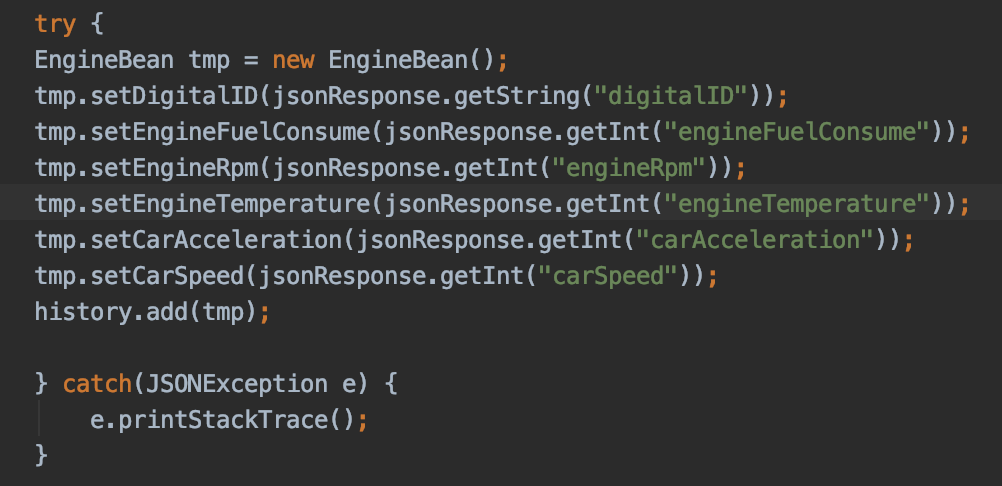
\includegraphics[width=1\textwidth]{img/history_screen.png}
    \caption{Salvataggio in sessione dei valori JSON di ritorno dal server REST}
    \label{fig:session_history}
\end{figure}
Si è scelto in fase implementativa di non disporre di meccanismi interni al chaincode per estrapolare i dati volta per volta dagli ultimi cinque blocchi della catena per l'assenza di una chiamata a sistema relativa al prelievo degli stati mantenuti nella storia del ledger. Gli ultimi aggiornamenti della libreria shim dispongono, nelle proprie API, una funzione denominata "getHistoryByKey" in cui preleva un insieme di coppie di valori relative ai dati della storia trasferita insieme ai timestamp del blocco di appartenza relativi a un entità definita dal valore della chiave passata in input. Di seguito mostriamo la dashboard finale corrispondente al monitoraggio della temperatura, del consumo di carburante di un motore e gli RPM dell'auto sotto analisi:
\newpage
\begin{figure}[h]
    \centering
    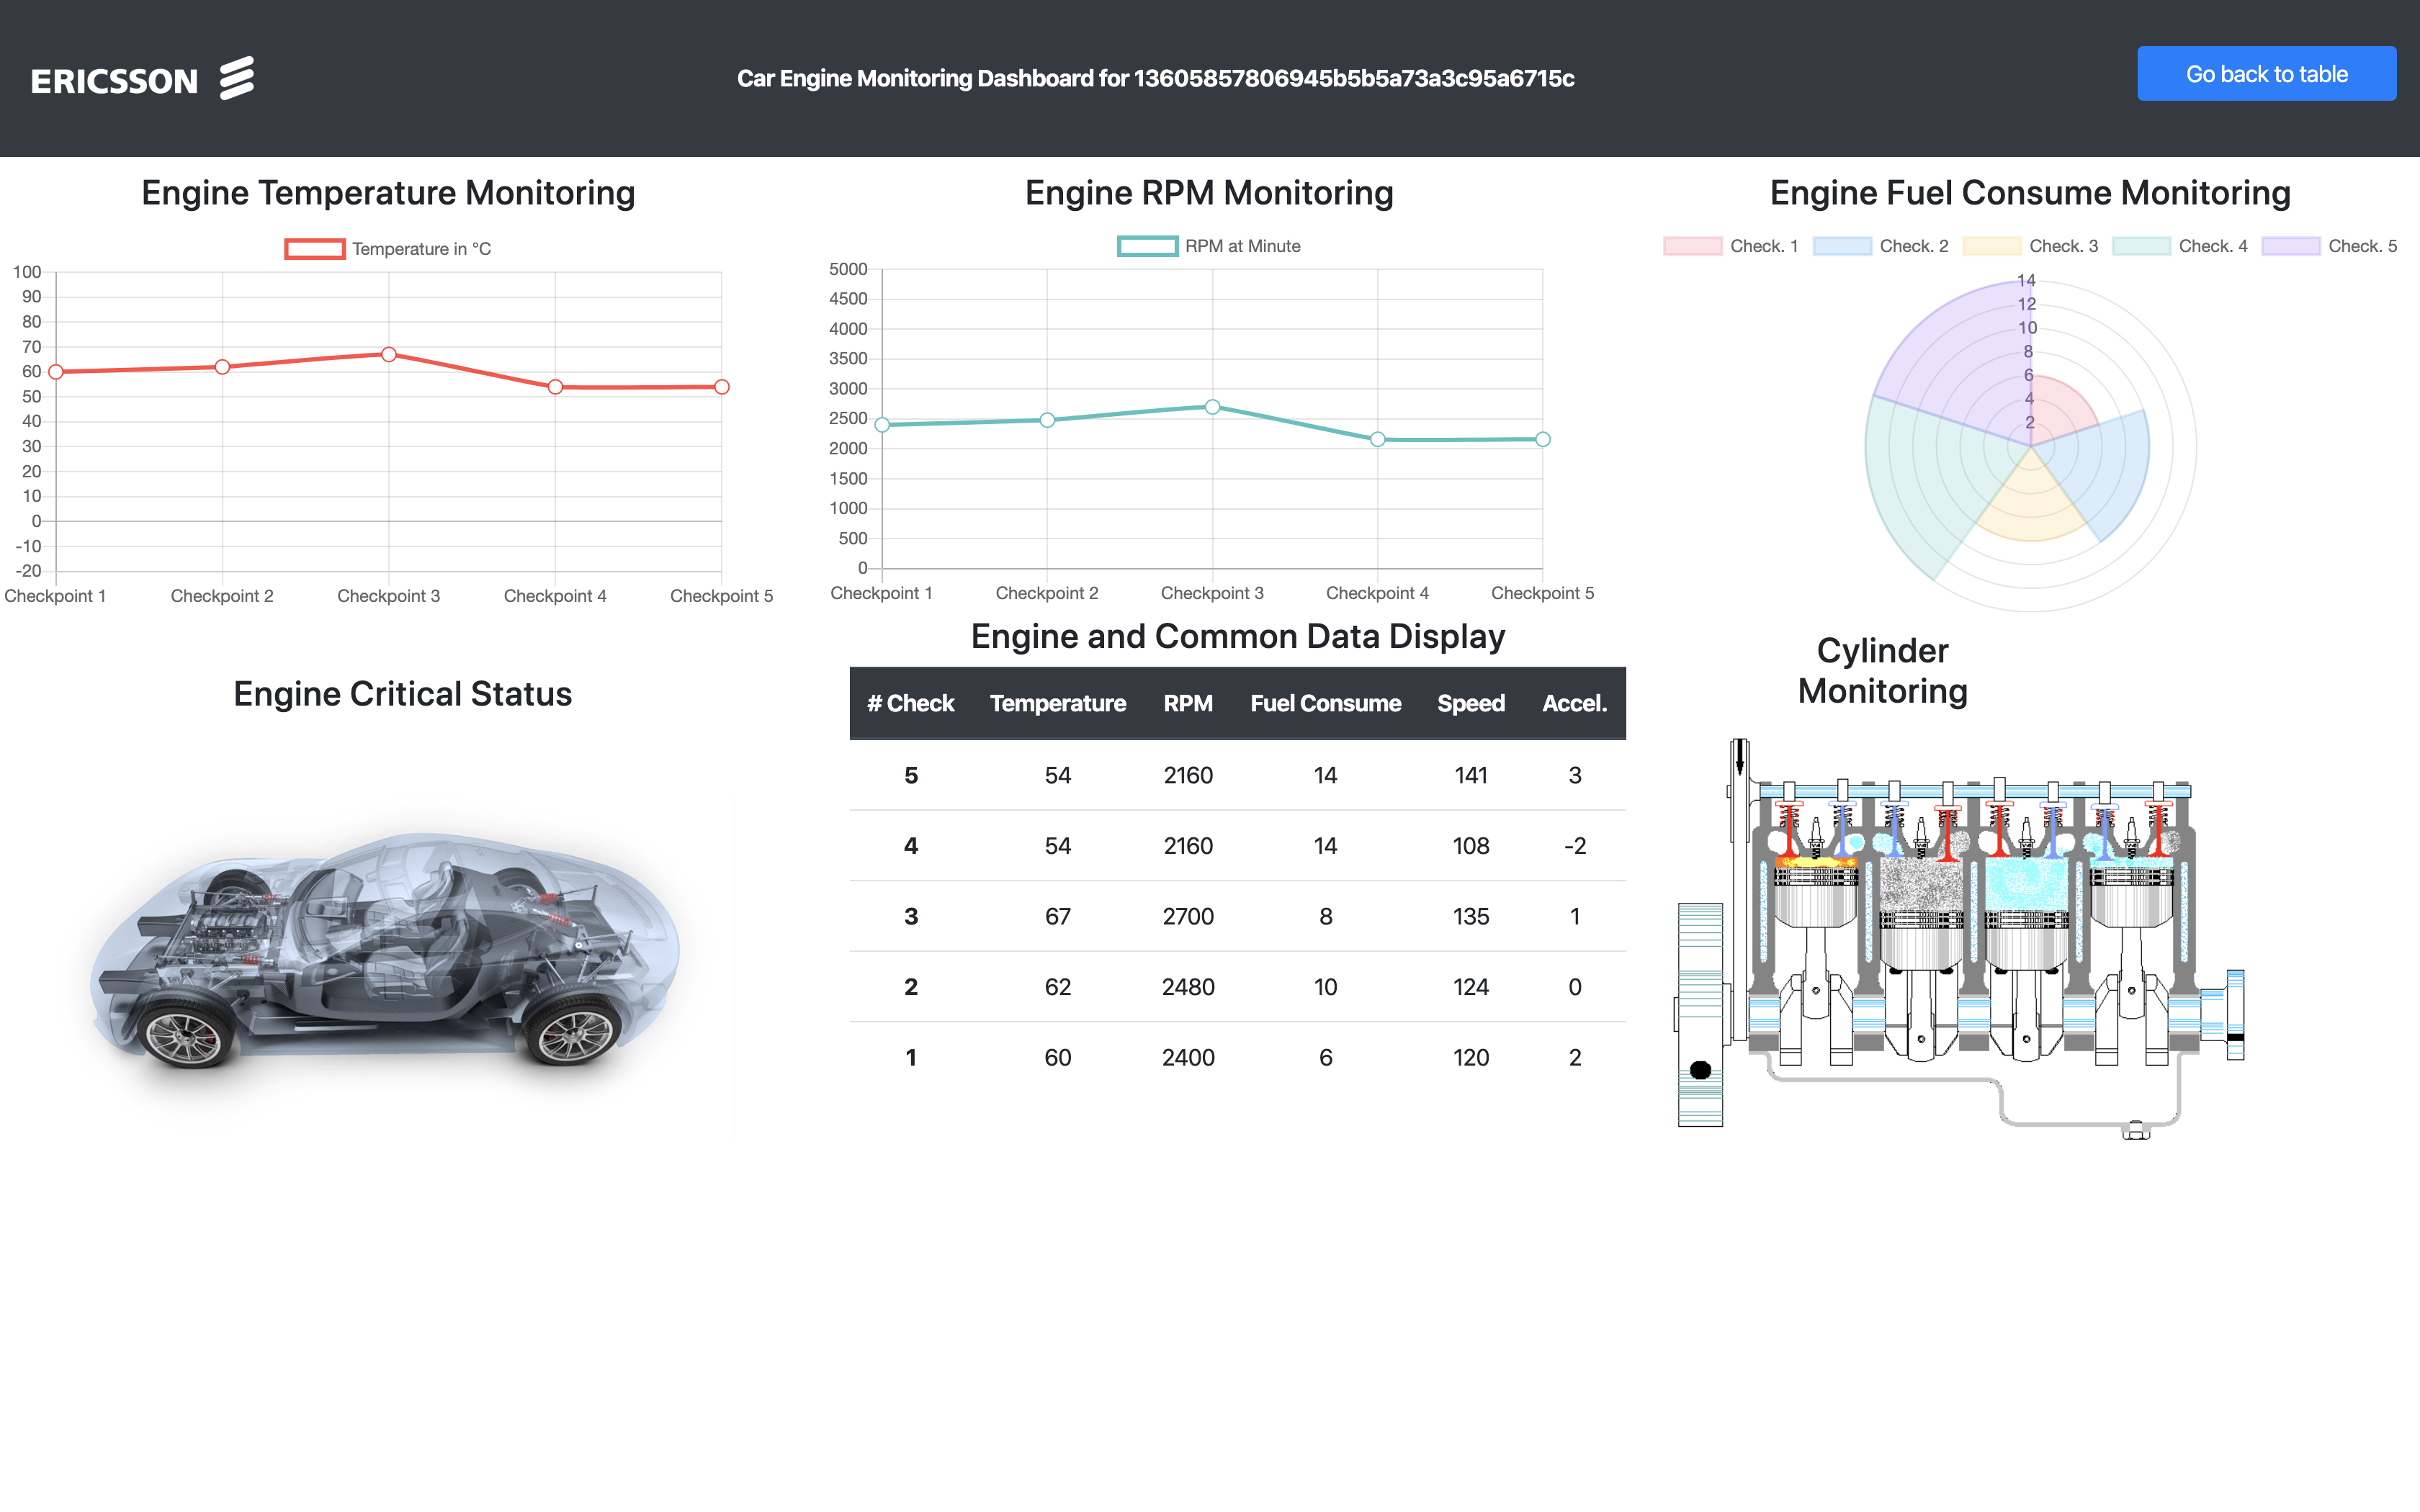
\includegraphics[width=1\textwidth]{img/engine_monitoring.png}
    \caption{Dashboard di monitoraggio per il motore di un'auto}
    \label{fig:dashboard_automotive}
\end{figure}
Le difficoltà maggiori che si sono riscontrate si basano sul dover adattare la frequenza di monitoraggio con la latenza dell'architettura poichè, per mantenere affidabilità, la blockchain ha bisogno di validare ogni blocco aggiunto dal simulatore. Tale meccanismo, anche se ad alte prestazioni, crea latenza all'interno della rete e, in fase di lettura, bisogna diminuire la frequenza per poter leggere i dati aggiornati in maniera corretta. 
\newpage
\section{Back-End}
L'implementazione delle componenti back-end si è concentrata sulla creazione di server REST che forniscono un'interfaccia pubblica di gestione per le varie funzioni invocabili di un chaincode installato sul canale della blockchain sottostante. Questa caratteristica è comune a entrambi i prototipi sviluppati che variano la propria interfaccia pubblica per: 
\begin{itemize}
    \item Funzione da invocare all'interno del chaincode
    \item Input da passare all'invocazione della funzione
    \item Output restituito
\end{itemize}
Le varie REST API che compongono il server definiscono tutte le operazioni che bisogna effettuare all'interno delle collezioni dello stato globale del ledger della blockchain offrendo un livello logico direttamente utilizzabile ai client. Se, però, i client non sono autorizzati a effettuare particolari funzioni del chaincode dello strato sottostante, la chiamata restituirà un errore di autorizzazione. Definiamo ora la struttura interna dell'implementazione di uno dei server REST implementati soffermandoci sulle operazioni d'interazione con la blockchain sottostante. 
I server REST sono basati sul framework Express.js per le operazioni di connessione asincrona sulle chiamate alle API offerte dal REST web service che si vuole creare. Utilizzeremo anche alcuni SDK (Software Developer Kit) tra cui "fabric-client" per definire le interazioni tra il server e le componenti della blockchain Fabric e "body-parser" per la gestione della formattazione del corpo della request all'interno di un middleware. Tramite SDK specifici, possiamo manipolare entità e proprietà proprie della blockchain Fabric, all'interno dell'implementazione si è stabilito, per ogni server, un peer di riferimento tra quelli dell'organizzazione su cui si interfaccia, l'orderer e il canale dell'architettura per la validazione e la sottomissione delle varie transazioni che si andranno a creare. 
Di seguito riportiamo il codice per l'instanziazione delle componenti logiche d'interazione con Fabric
\begin{figure}[h]
    \centering
    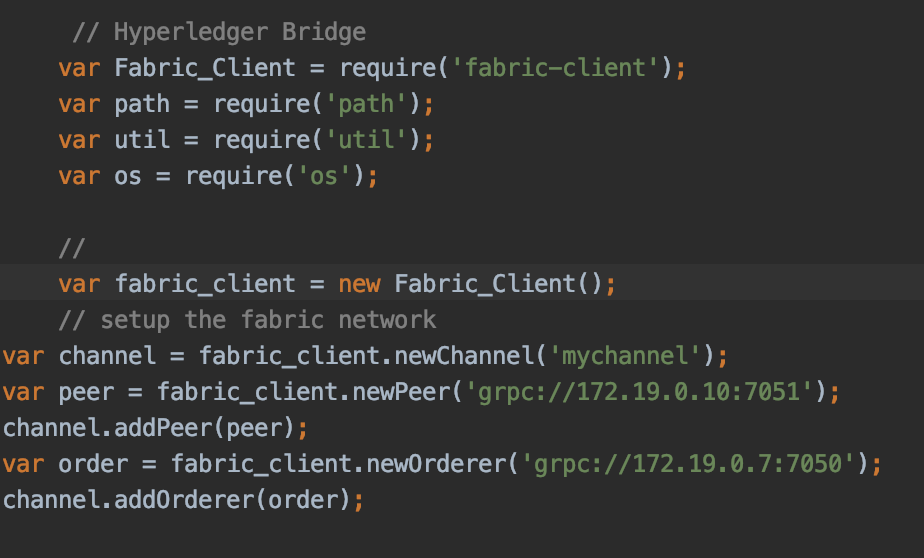
\includegraphics[width=1\textwidth]{img/express-comp-fabric.png}
    \caption{Snippet di codice per l'instanziazione delle componenti logiche di Fabric interessate nella comunicazione con il server REST}
    \label{snippet-comp-fabric}
\end{figure}
\newpage
Per mantenere la logica architetturale propria di Fabric, ogni REST API  deve poter rispettare le seguenti proprietà: 
\begin{enumerate}
    \item Bisogna adottare un meccanismo che richiami le CA di Fabric per mantenere i criteri di autenticazione e di autorizzazione.
    \item Prima di inviare una transazione che aggiorna lo stato globale del ledger della blockchain, bisogna inviare una proposta di transazione e gestire i possibili risultati del consenso. 
    \item Creare e gestire la transazione andando ad invocare una funzione del chaincode e propagare il risultato al client all'interno della response della REST API. 
\end{enumerate}
All'interno del prototipo, la logica di autenticazione prevede l'estrapolazione della chiavi di autenticazione all'interno di un wallet locale andando a richiamare un contesto legato ad un singolo utente, ciò sta a significare che ogni richiesta di transazione proveniente dal server REST e mantenuta all'interno del ledger di Fabric verrà segnata con la firma dell'utente del prototipo. 
\begin{figure}[h]
    \centering
    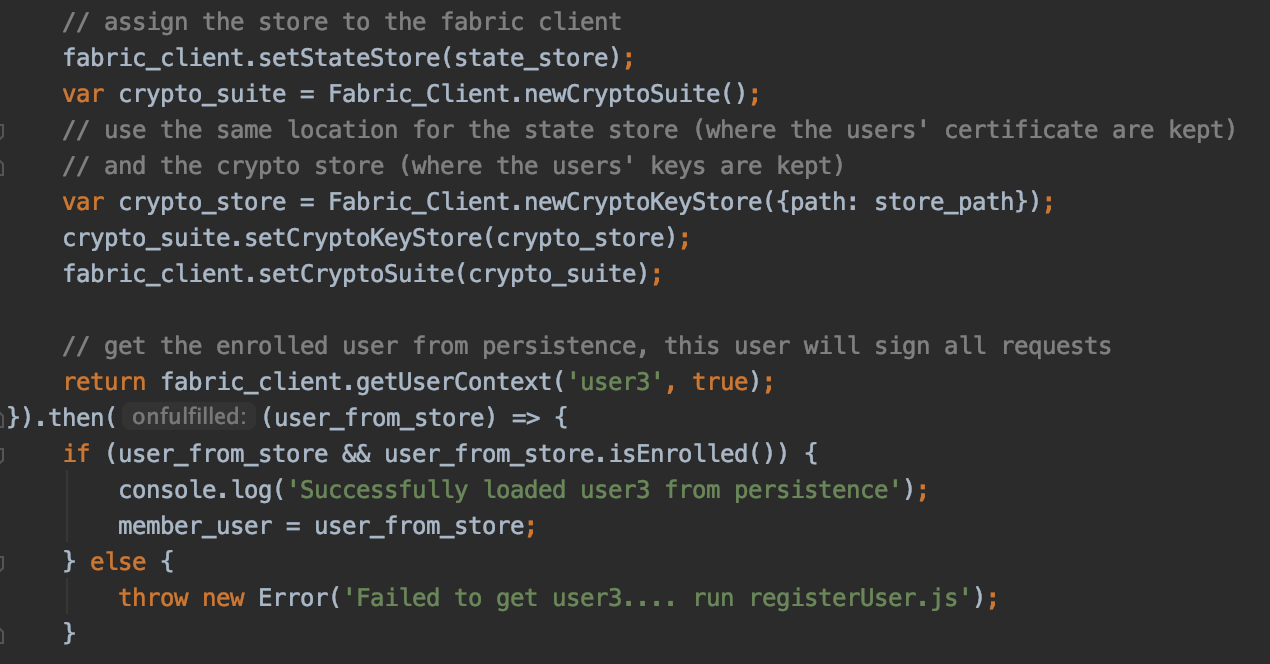
\includegraphics[width=1\textwidth]{img/aut-server.png}
    \caption{Snippet di codice l'autenticazione per la gestione delle signature di un'utente di esempio mantenuto in un wallet del prototipo}
    \label{autent-express-server}
\end{figure}
In seguito all'impostazione per rispettare il criterio di autenticazione, i server REST formattano la richiesta che andrà in input al chaincode in modo da poter invocare una specifica funzione andando a passare i parametri di input richiesti. Tale richiesta andrà ad essere inviata nella proposta di transazione e verificata nel seguente modo:

\begin{figure}[h]
    \centering
    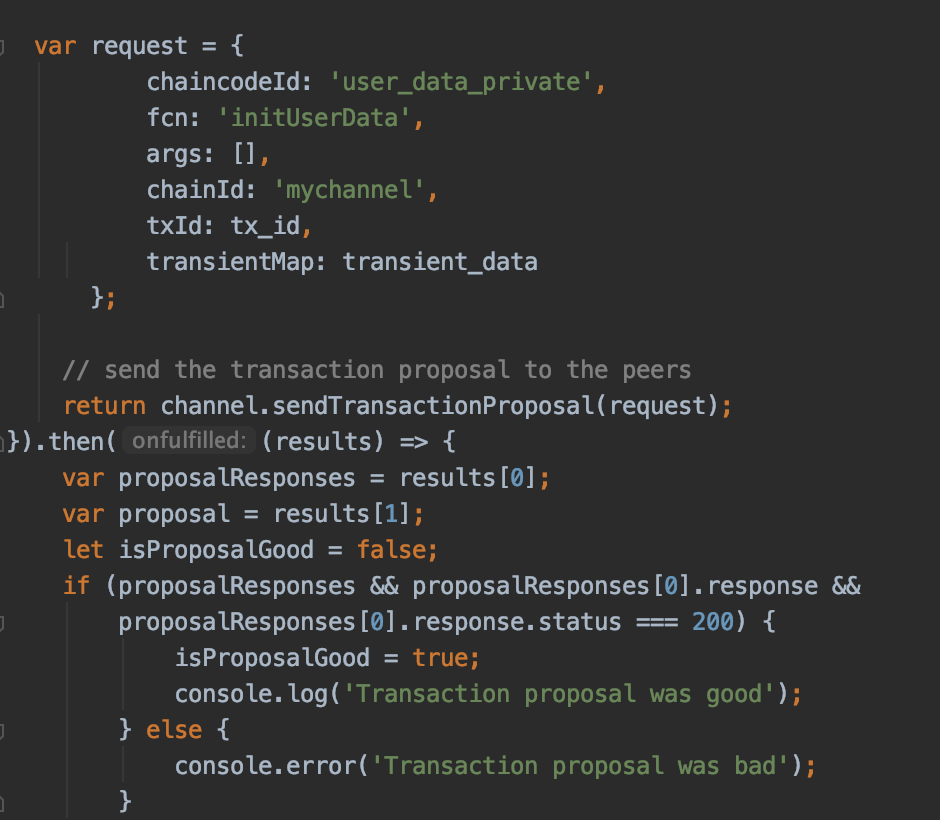
\includegraphics[width=0.5\textwidth]{img/proposal-request.png}
    \caption{Snippet di codice di gestione della proposta di transazione}
    \label{proposal-script}
\end{figure}
Se la proposta è andata a buon fine, viene definita una richiesta di transazione contente la risposta della proposta di transazione insieme ai dati di input e alle informazioni di invocazione. La richiesta di transazione viene inviata all'orderer per il commit della transazione in modo da effettuare l'aggiunta di un blocco di transazione che andrà ad aggiornare le istanze del ledger di ogni peer della blockchain. La transazione andrà a modificare lo stato globale delle istanze dei ledger dei peer della rete solamente se l'operazione è di scrittura. La REST API riceverà in risposta l'output della transazione e, a secondo se sia considerata valida o meno, verrà inoltrato una specifica risposta al client: 
\begin{figure}[h]
    \centering
    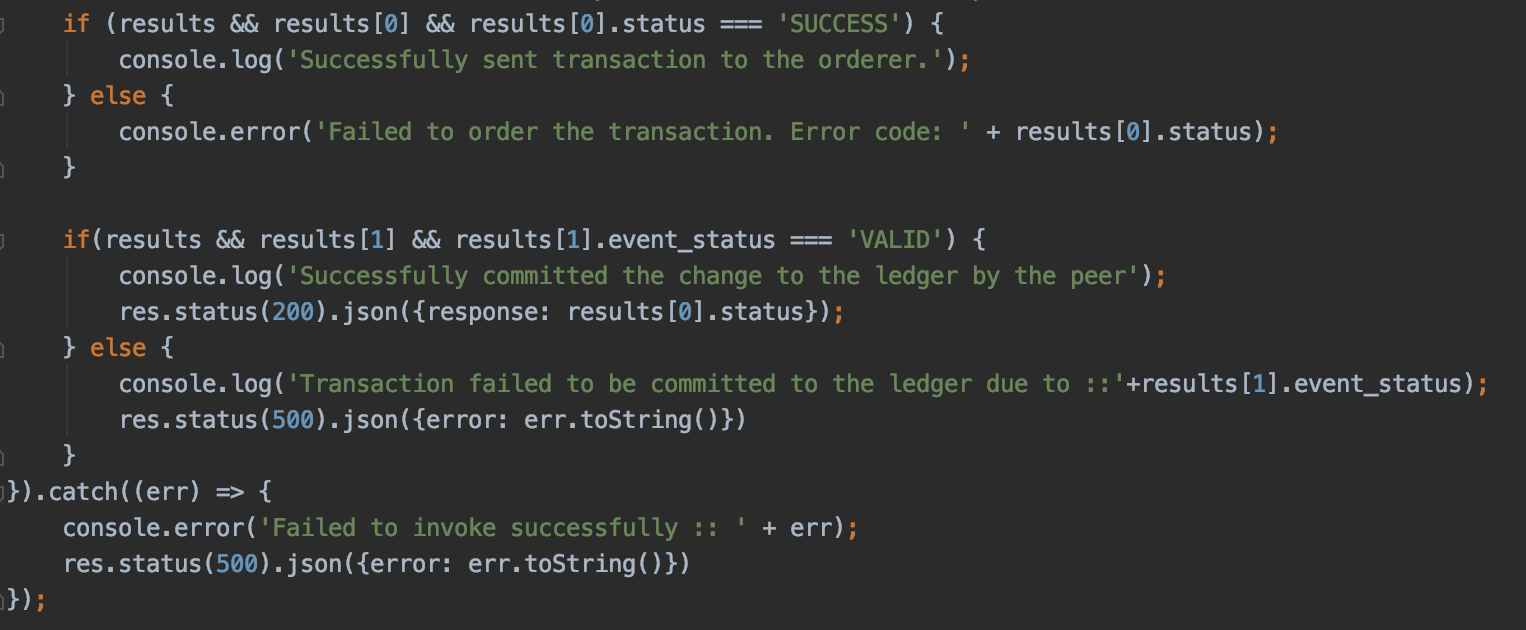
\includegraphics[width=1\textwidth]{img/response-result.png}
    \caption{Gestione della risposta ad una REST API}
    \label{result-script}
\end{figure}
\newpage
\section{Rete basata su Hyperledger Fabric}
All'interno di questo paragrafo andiamo a definire tutta la configurazione dell'architettura Fabric implementata all'interno dei prototipi. Poichè non vi è distinzione all'interno della struttura della blockchain tra i due prototipi implementati, non si avranno distinzione tra i due casi d'uso.
\subsection{Script di inizializzazione}
La rete su cui è basata la blockchain è formata da due organizzazioni, un canale, un orderer, quattro peer (due per ogni organizzazione), un interfaccia a riga di comando, un'istanza di un database di stato del leger basato su couchdb e due istanze dei chaincode montate su ogni organizzazione. La composizione dei container si basa sulla struttura del progetto "first-network" disponibile in open-source. 
\begin{figure}[h]
    \centering
    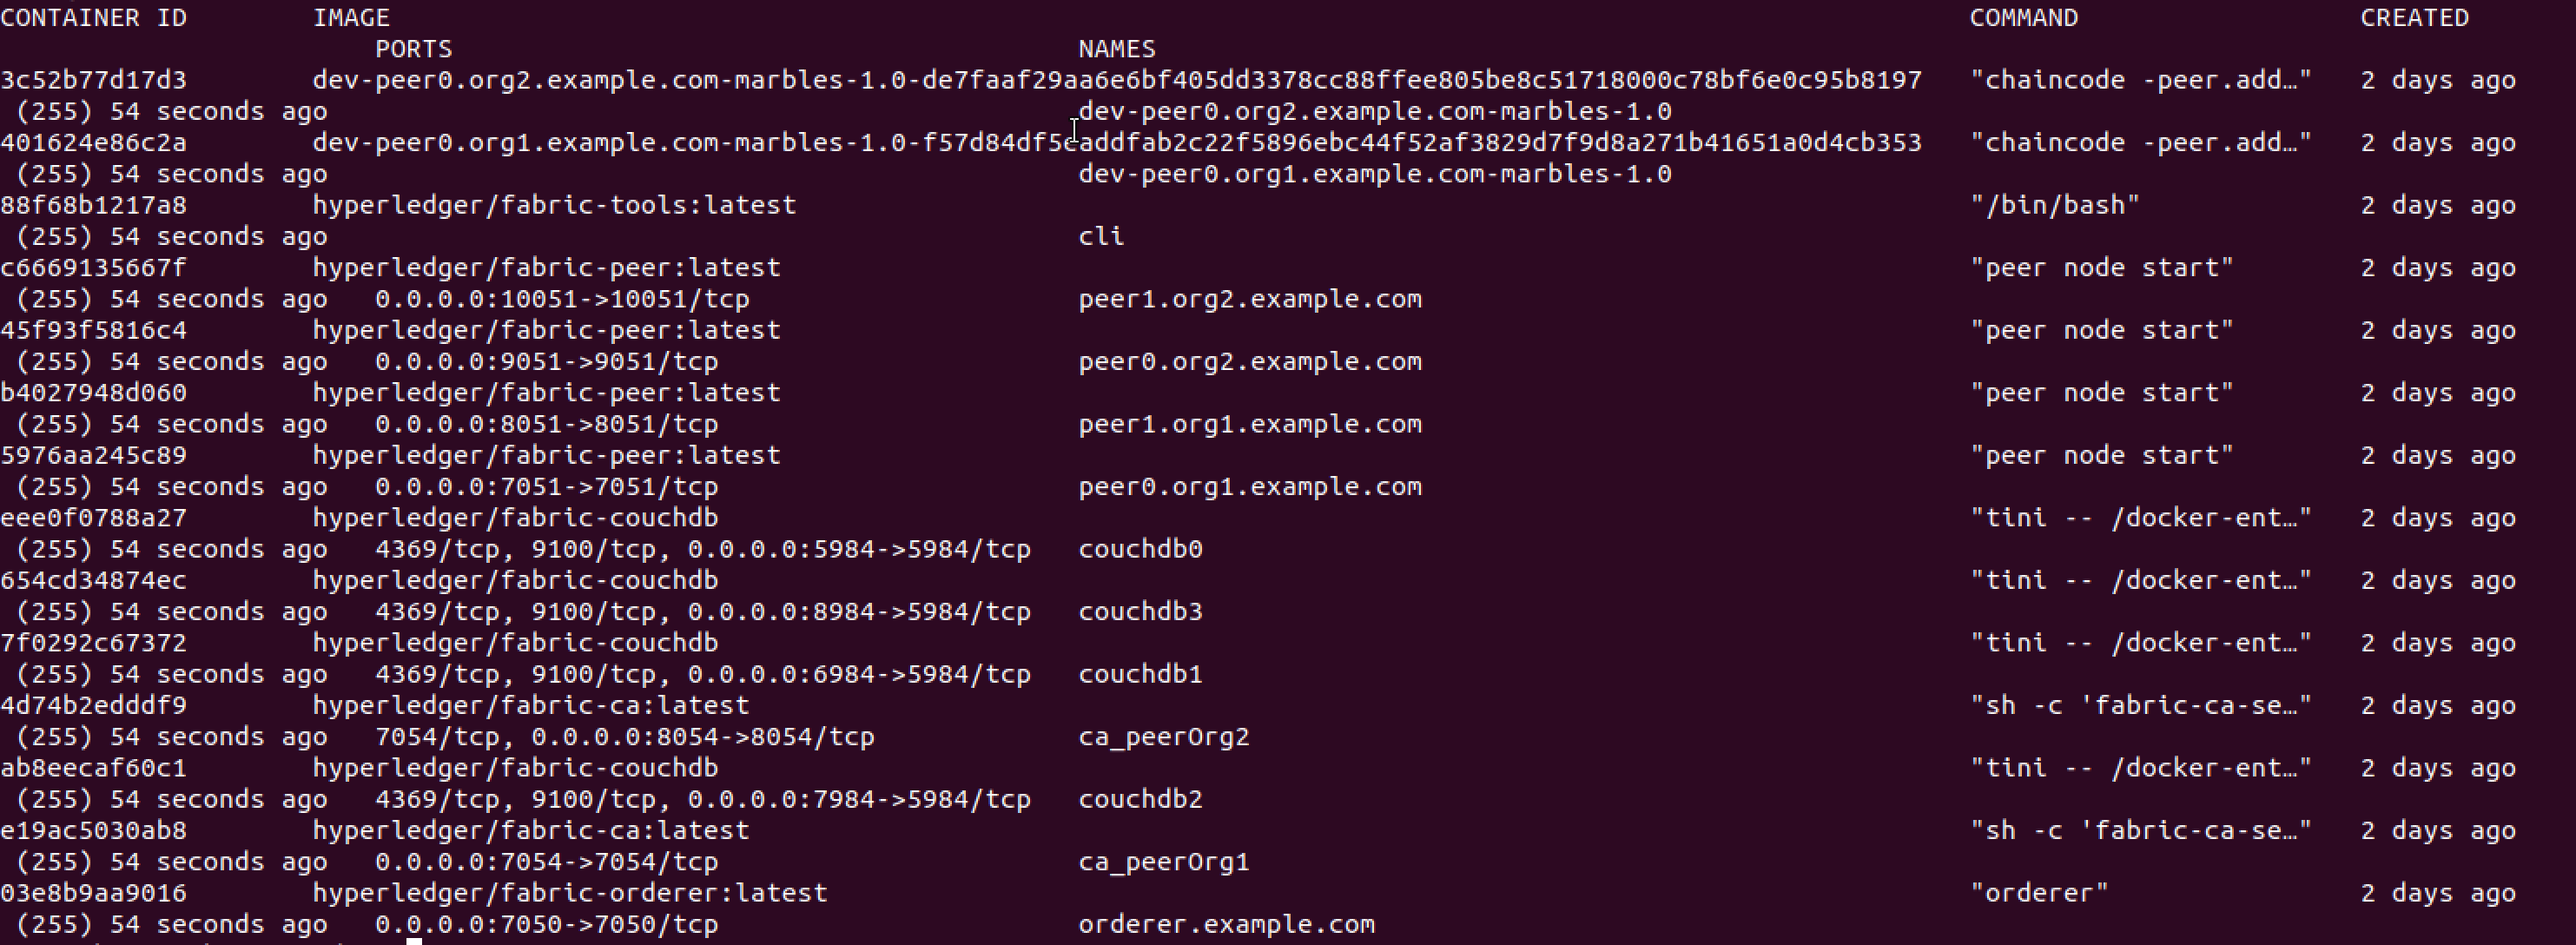
\includegraphics[width=1\textwidth]{img/docker-impl.png}
    \caption{Composizione dei container Docker per l'implementazione della rete blockchain}
    \label{fig:docker-impl}
\end{figure}
Gli script di inizializzazione lavorano in linguaggio shell, andando a definire una serie di comandi che inizializzano i container andando ad effettuare il caricamento delle applicazioni che montano le varie componenti sulla rete. 
Per entrambi i prototipi, la struttura di base è come quella appena descritta. Per eseguire l'inzi pt shell tramite un comando dal terminale Linux: 
\begin{verbatim}
    ./byfn.sh up -c mychannel -s couchdb
\end{verbatim}
L'esecuzione dello script di inizializzazione prende in input l'operazione da eseguire e due flag che definiscono il nome del canale da definire e la configurazione del tipo di database per mantenere le istanze dello stato globale del ledger sui vari peer di rete.
\subsection{File di configurazione}
Nello specifico, l'esecuzione consiste nel richiamare dei file di configurazioni in linguaggio YAML tramite il comando "docker-compose" in cui sono contenute le specifiche dei servizi da montare all'interno dei container. 
I tipi di file YAML implementati rappresentano delle policy strutturali che fanno riferimento ai seguenti concetti:
\begin{enumerate}
    \item Caratteristiche delle immagini delle componenti di base di un'organizzazione: MSP, Peer, autorità di certificazione, database di stato
    \item Configurazione della struttura del CA: Andando a definire le proprietà su cui si basano le autorità di certificazione
    \item Interfaccia a linea di comando: Definendo le proprietà dell'immagine dell'interfaccia a linea di comando da caricare. 
\end{enumerate}
Nei paragrafi successivi andremo ad analizzare ogni tipo di file YAML sotto un punto di vista implementativo. 
\subsubsection{File di configurazione delle immagini delle componenti di base}
\begin{figure}[h]
    \centering
    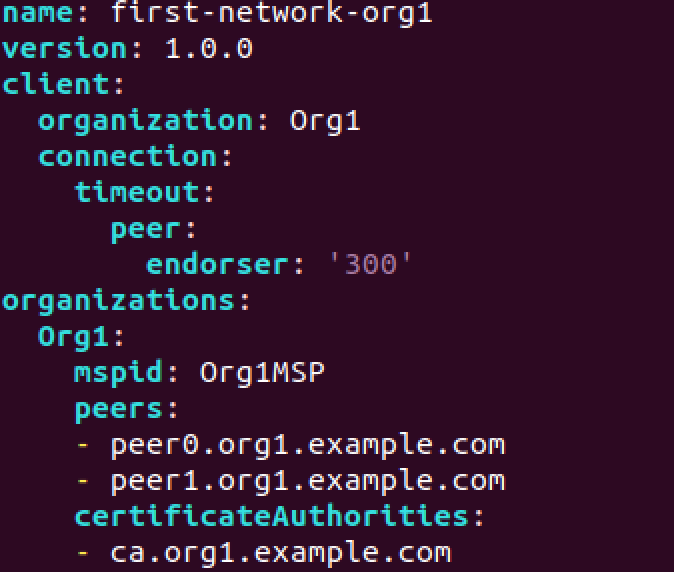
\includegraphics[width=0.5\textwidth]{img/connection-config-yaml.png}
    \caption{Snippet di codice YAML per la configurazione delle componenti di base di un'organizzazione mantenute nel file connection-org1.yaml}
    \label{fig:connection-config-yaml}
\end{figure}
Il file di configurazione delle immagini delle componenti di base di un'organizzazione è  definisce le proprietà per le seguenti entità di rete: 
\begin{itemize}
    \item Organizzazione: Consiste nelle specifiche dell'ID nominativo dell'entità, i riferimenti ai nomi dei peer, del CA e del MSP. 
    \item Peer: Consiste nelle specifiche dell'url, del nome logico, dei certificati di accesso e di opzioni del protocollo di comunicazione interno alla blockchain.
    \item CA: Consiste nelle specifiche dell'url, del nome di riferimento, del certificato di accesso e delle opzioni del protocollo di comunicazione con applicazioni esterne. 
\end{itemize}
All'interno dell'implementazione di entrambi i prototipi sviluppati, si è utilizzato il protocollo GRPC per la comunicazione interna e il protocollo HTTP per la comunicazione esterna che, nel nostro caso, fa riferimento ai server REST di interfacciamento alle funzioni delle istanze dei chaincode montate su ogni peer. 
\subsubsection{Configurazione della struttura del CA}
Il file YAML legato alla configurazione della struttura del CA definisce le proprietà dell'autorità di certificazione, le principali sono: 
\begin{itemize}
    \item Immagine su cui si basa ogni CA
    \item Variabili di Ambiente
    \item Porte di Comunicazione I/O
    \item Nome del Container
\end{itemize}
Mentre per la configurazione delle componenti di base si ha solamente la definizione delle componenti su cui agiscono i CA (certificati, host di accesso). All'interno della configurazione della loro struttura, si specificano tutte le proprietà logiche utilizzate per poter eseguire correttamente il meccanismo di autenticazione. Si è deciso di non distinguere il file di configurazione delle CA dandone solamente una definizione in modo che tutte le organizzazioni abbiano gli stessi meccanismi di accesso. 
\begin{figure}[h]
    \centering
    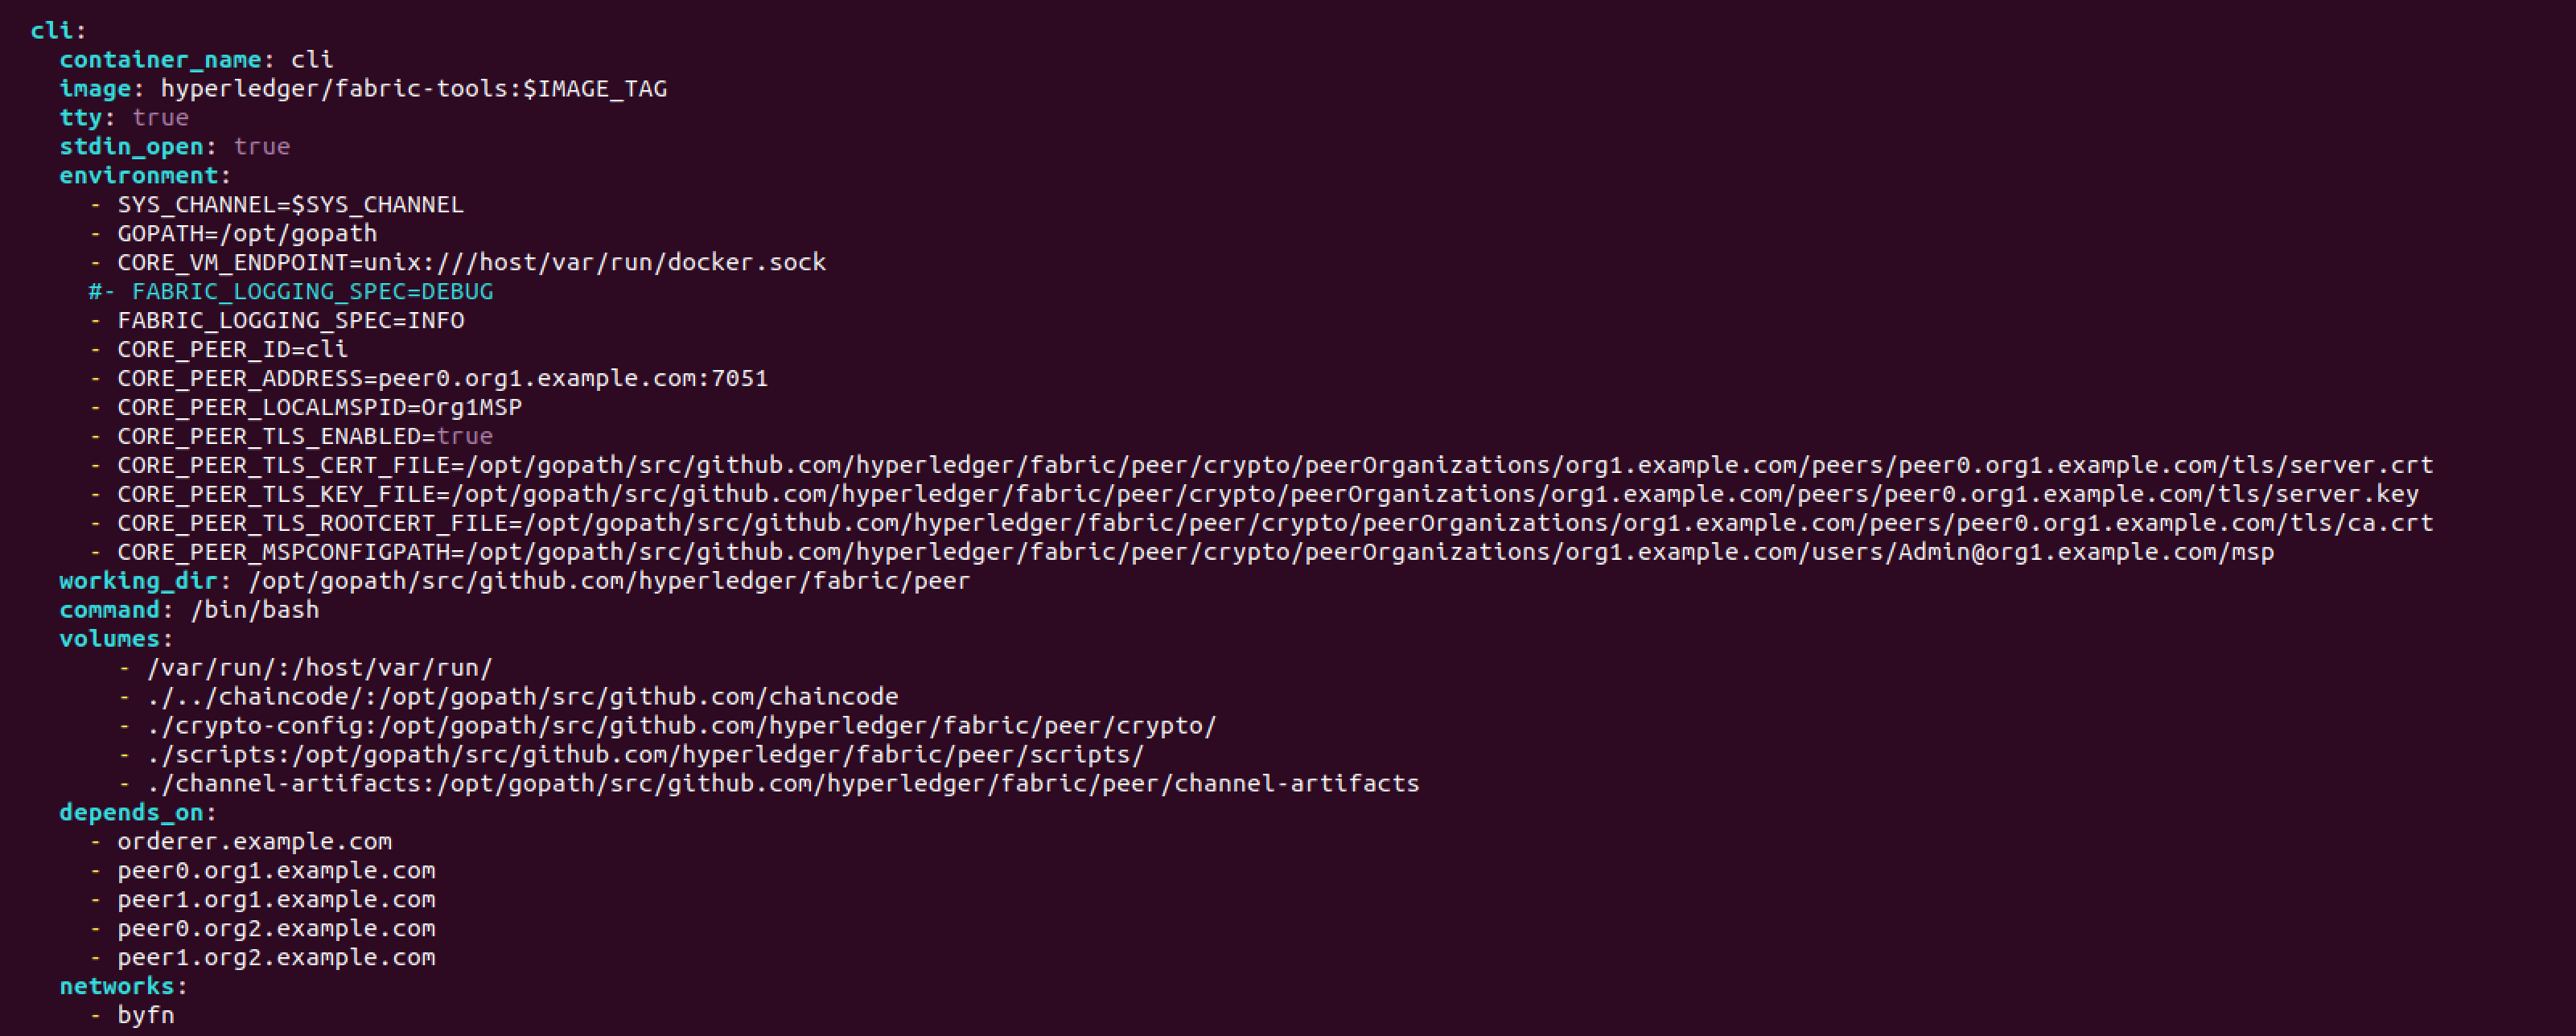
\includegraphics[width=1\textwidth]{img/docker-compose-cli-yaml.png}
    \caption{Snippet di codice YAML per la configurazione del CLI}
    \label{fig:connection-cli-yaml}
\end{figure}
\subsubsection{File di configurazione del CLI}
Il file YAML di configurazione del CLI della rete Fabric, denominato docker-compose-cli.yaml all'interno dei prototipi del progetto, è stato implementato  andando a specificare le seguenti proprietà: 
\begin{itemize}
    \item Nome del container
    \item Immagine del container
    \item Dipendenze
    \item Variabili di Ambiente
\end{itemize}
All'interno dei riferimenti ai volumi delle entità in cui può accedere il CLI, si ha che alcune proprietà  sono state isolate all'interno di un'ulteriore file di configurazione secondario chiamato "docker-compose-base.yaml" in cui poter trovare le caratteristiche di base dei servizi dipendenti come i peer di un'organizzazione o un'orderer.
\subsection{Gestione del chaincode}
Il chaincode viene definito tramite un file in linguaggio Golang istanziato in maniera distribuita sui vari peer delle organizzazioni partecipanti ad un canale sulla blockchain, la sua implementazione si concentra sulla definizione dei seguenti concetti: 
\begin{enumerate}
    \item Struttura delle collezioni di dati mantenute dentro lo stato globale del ledger
    \item Funzione di invocazione del chaincode
    \item Operazioni di business per la manipolazione dello stato globale
\end{enumerate}
\subsubsection{Struttura delle collezioni}
\begin{figure}[h]
    \centering
    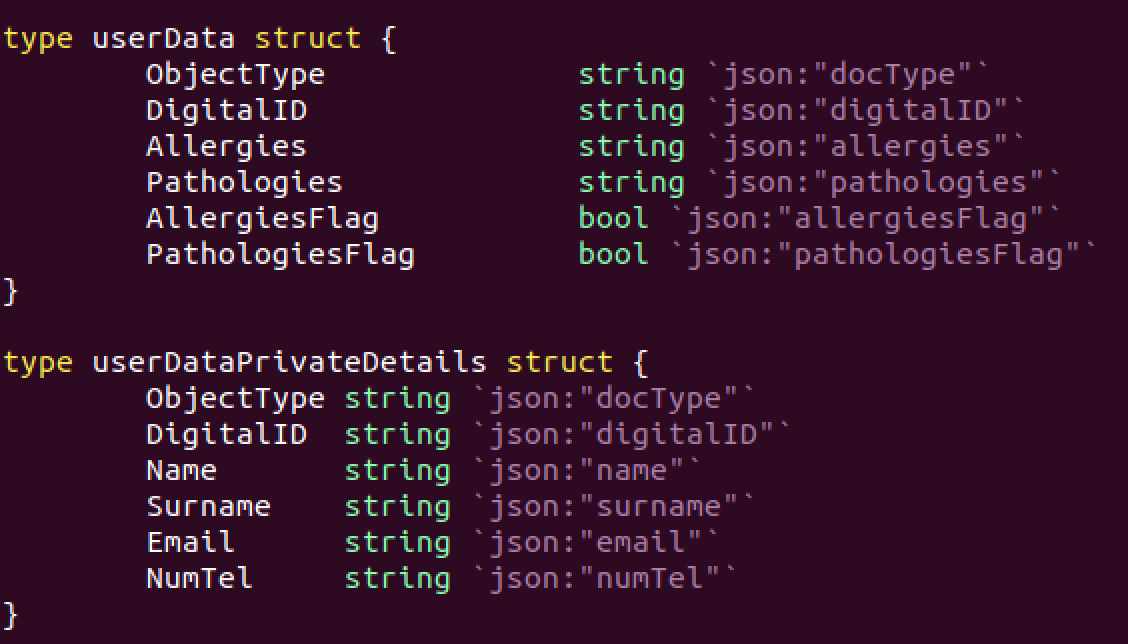
\includegraphics[width=0.8\textwidth]{img/collection-chaincode.png}
    \caption{Definizione della collezione all'interno del caso d'uso sanitario}
    \label{fig:collection-chaincode}
\end{figure}
\begin{figure}[h]
    \centering
    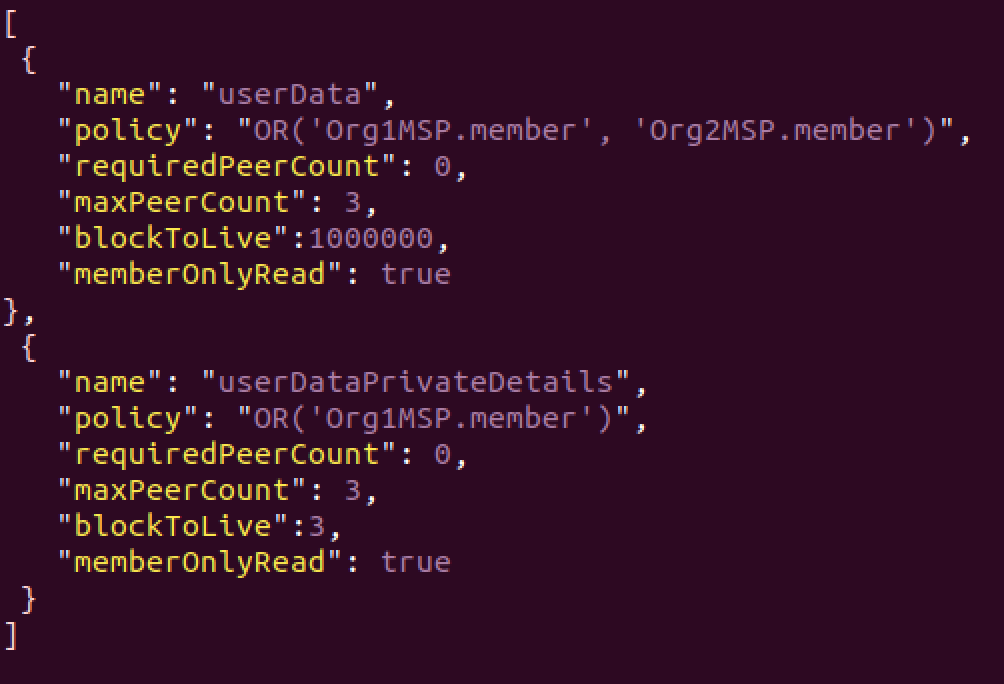
\includegraphics[width=0.8\textwidth]{img/policy-collection-json.png}
    \caption{Definizione delle policy di accesso per le collezioni del caso d'uso sanitario}
    \label{fig:policy-collection}
\end{figure}
In fase implementativa, le collezioni sono state definite come delle strutture dati globali.
Dentro il chaincode non vi è nessuna distinzione tra quali siano le collezioni private e quali pubbliche e nessun criterio di autorizzazione per verificare chi può o meno accedere, le politiche di gestione vengono specificate all'interno di un file di configurazione JSON esterno che definisce le policy di visibilità di una collezione. Tale file mantiene un array JSON in cui ogni elemento definisce i criteri di autenticazione specificati all'interno del paragrafo 3.5.2. Le collezioni private hanno un tempo di vita di blocco molto breve per evitare di andare a rendere reperibile i cambiamenti di stato tramite l'estrapolazione della storia della blockchain. Altre considerazioni implementative sono i riferimenti ai diritti di lettura in cui sono limitati solamente agli attori proprietari dei client d'interfacciamento, visibili dalla blockchain con il ruolo di membri semplici. Per la scrittura, invece, non vi sono limitazioni sui tipi di attori che possono effettuare tale operazione.

\newpage
\newpage
\subsubsection{Funzioni di invocazione}
\begin{figure}[h]
    \centering
    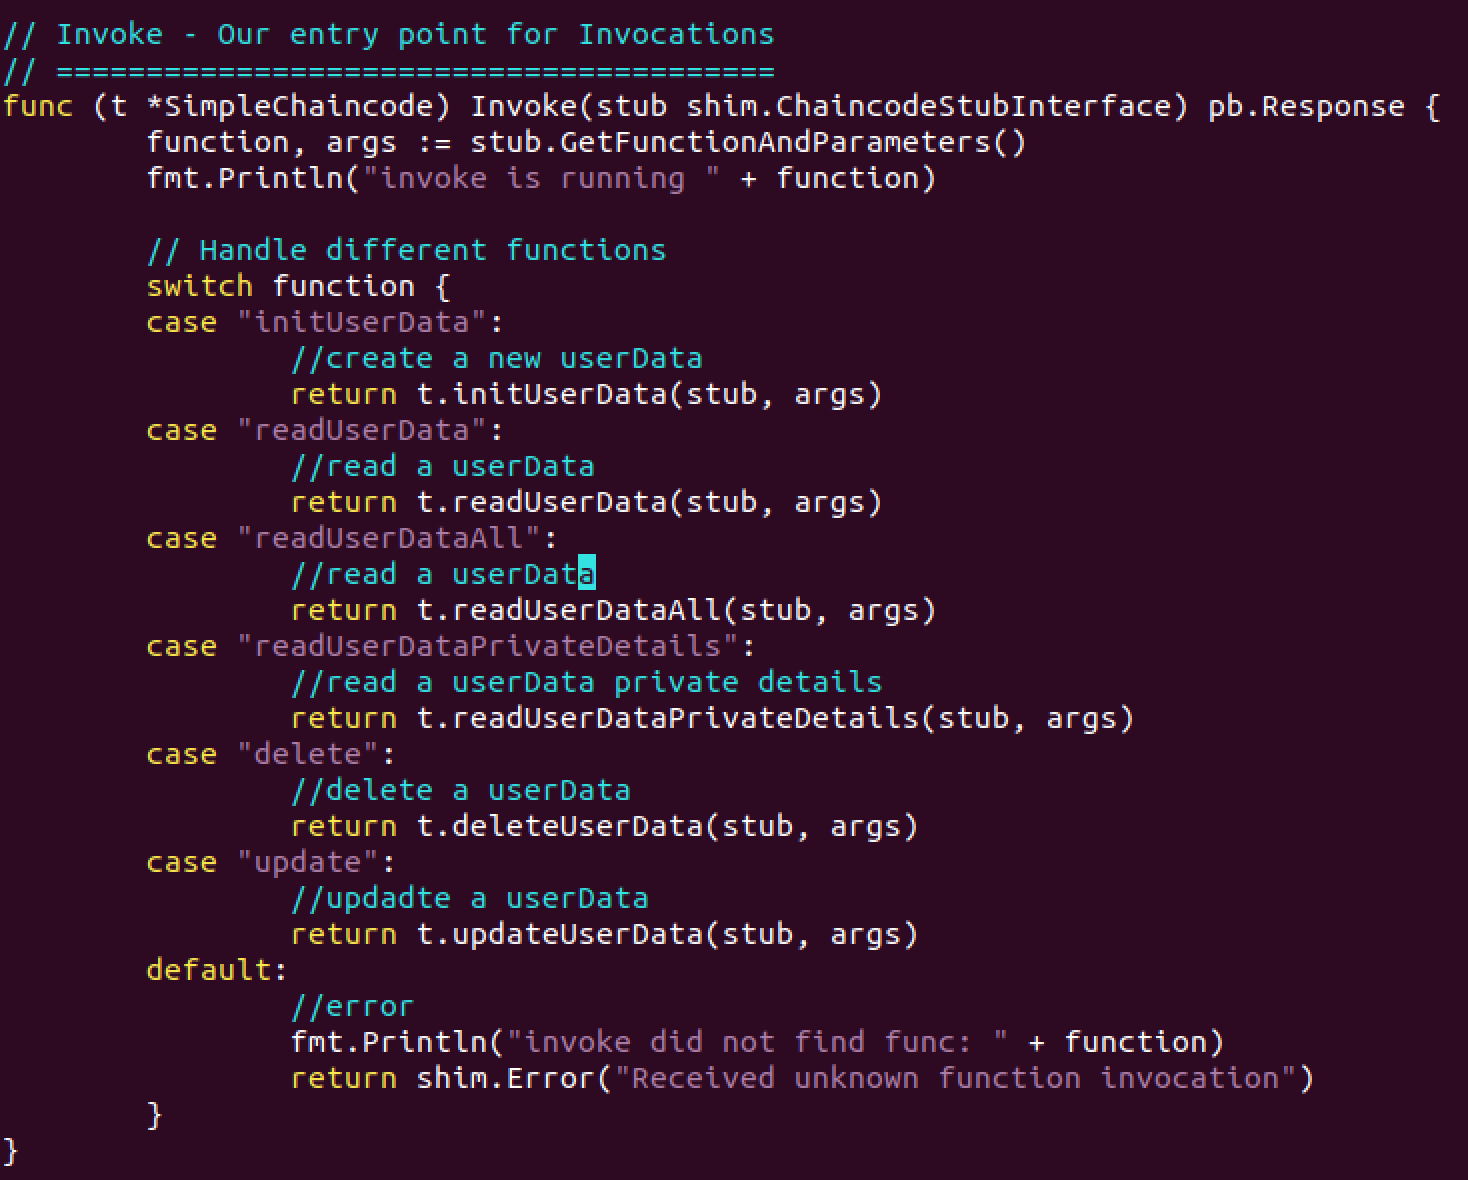
\includegraphics[width=0.8\textwidth]{img/invoke-chaincode.png}
    \caption{Funzione di invocazione nel chaincode della rete del prototipo sanitario}
    \label{fig:invoke-chaincode}
\end{figure}
La funzione d'invocazione nel chaincode viene richiamata ogni qualvolta si tende invocare un'operazione di business, l'implementazione di tale funzione prevede la gestione di inoltramento verso la chiamata della funzione del chaincode corrispondente andando a inoltrare l'interfaccia stub del chaincode e i parametri di input. La funzione GetFunctionAndParameters viene utilizzata per prendere i campi corrispondenti all'interno della struttura della request della REST API attraverso lo stub del chaincode. La libreria shim ha anche delle funzioni di controllo sulla richiesta che possono definire l'identità del chiamante e andare ad analizzare il suo ID per poter decidere già all'interno di tale funzione se un client sia autorizzato o meno. Nel caso dei prototipi, invece, si accede alla funzione e si controlla l'autorizzazione solamente quando si invocano le funzioni di alterazione o di accesso dello stato globale del ledger, ossia quando si accede alla copia del couchdb del peer richiamato.
\newpage
\subsubsection{Operazioni di business}
Le operazioni di business sono state implementate tramite varie funzioni che possono essere categorizzate in due grandi tipi: lettura e scrittura. Se l'operazione è di lettura, si riceve in input l'ID corrispondenti ad un oggetto JSON salvato all'interno del couchdb rappresentante lo stato globale del ledger. Se l'operazione è di scrittura, si riceve in input una struttura dati corrispondente ai dati delle collezione da sovrascrivere. L'operazione di modifica si identifica come un'operazione di scrittura in cui si ha la sovrascrizione dei dati di un particolare oggetto JSON salvato all'interno dello stato globale. Questa peculiarità ha come risultato quello di poter visualizzare, all'interno della storia del ledger, tutte le sovrascrizioni effettuate su un particolare oggetto a secondo del tempo di vita del blocco specificato dentro il file di configurazione della collezione di cui fa parte. Per quanto riguarda gli output delle funzioni, se l'operazione è di lettura si ritornano i dati letti dal ledger altrimenti, nel caso di un'operazione di scrittura, si darà in output un valore di stato che differisce a secondo se la procedura è andata a buon fine o meno.
\begin{figure}[h]
    \centering
    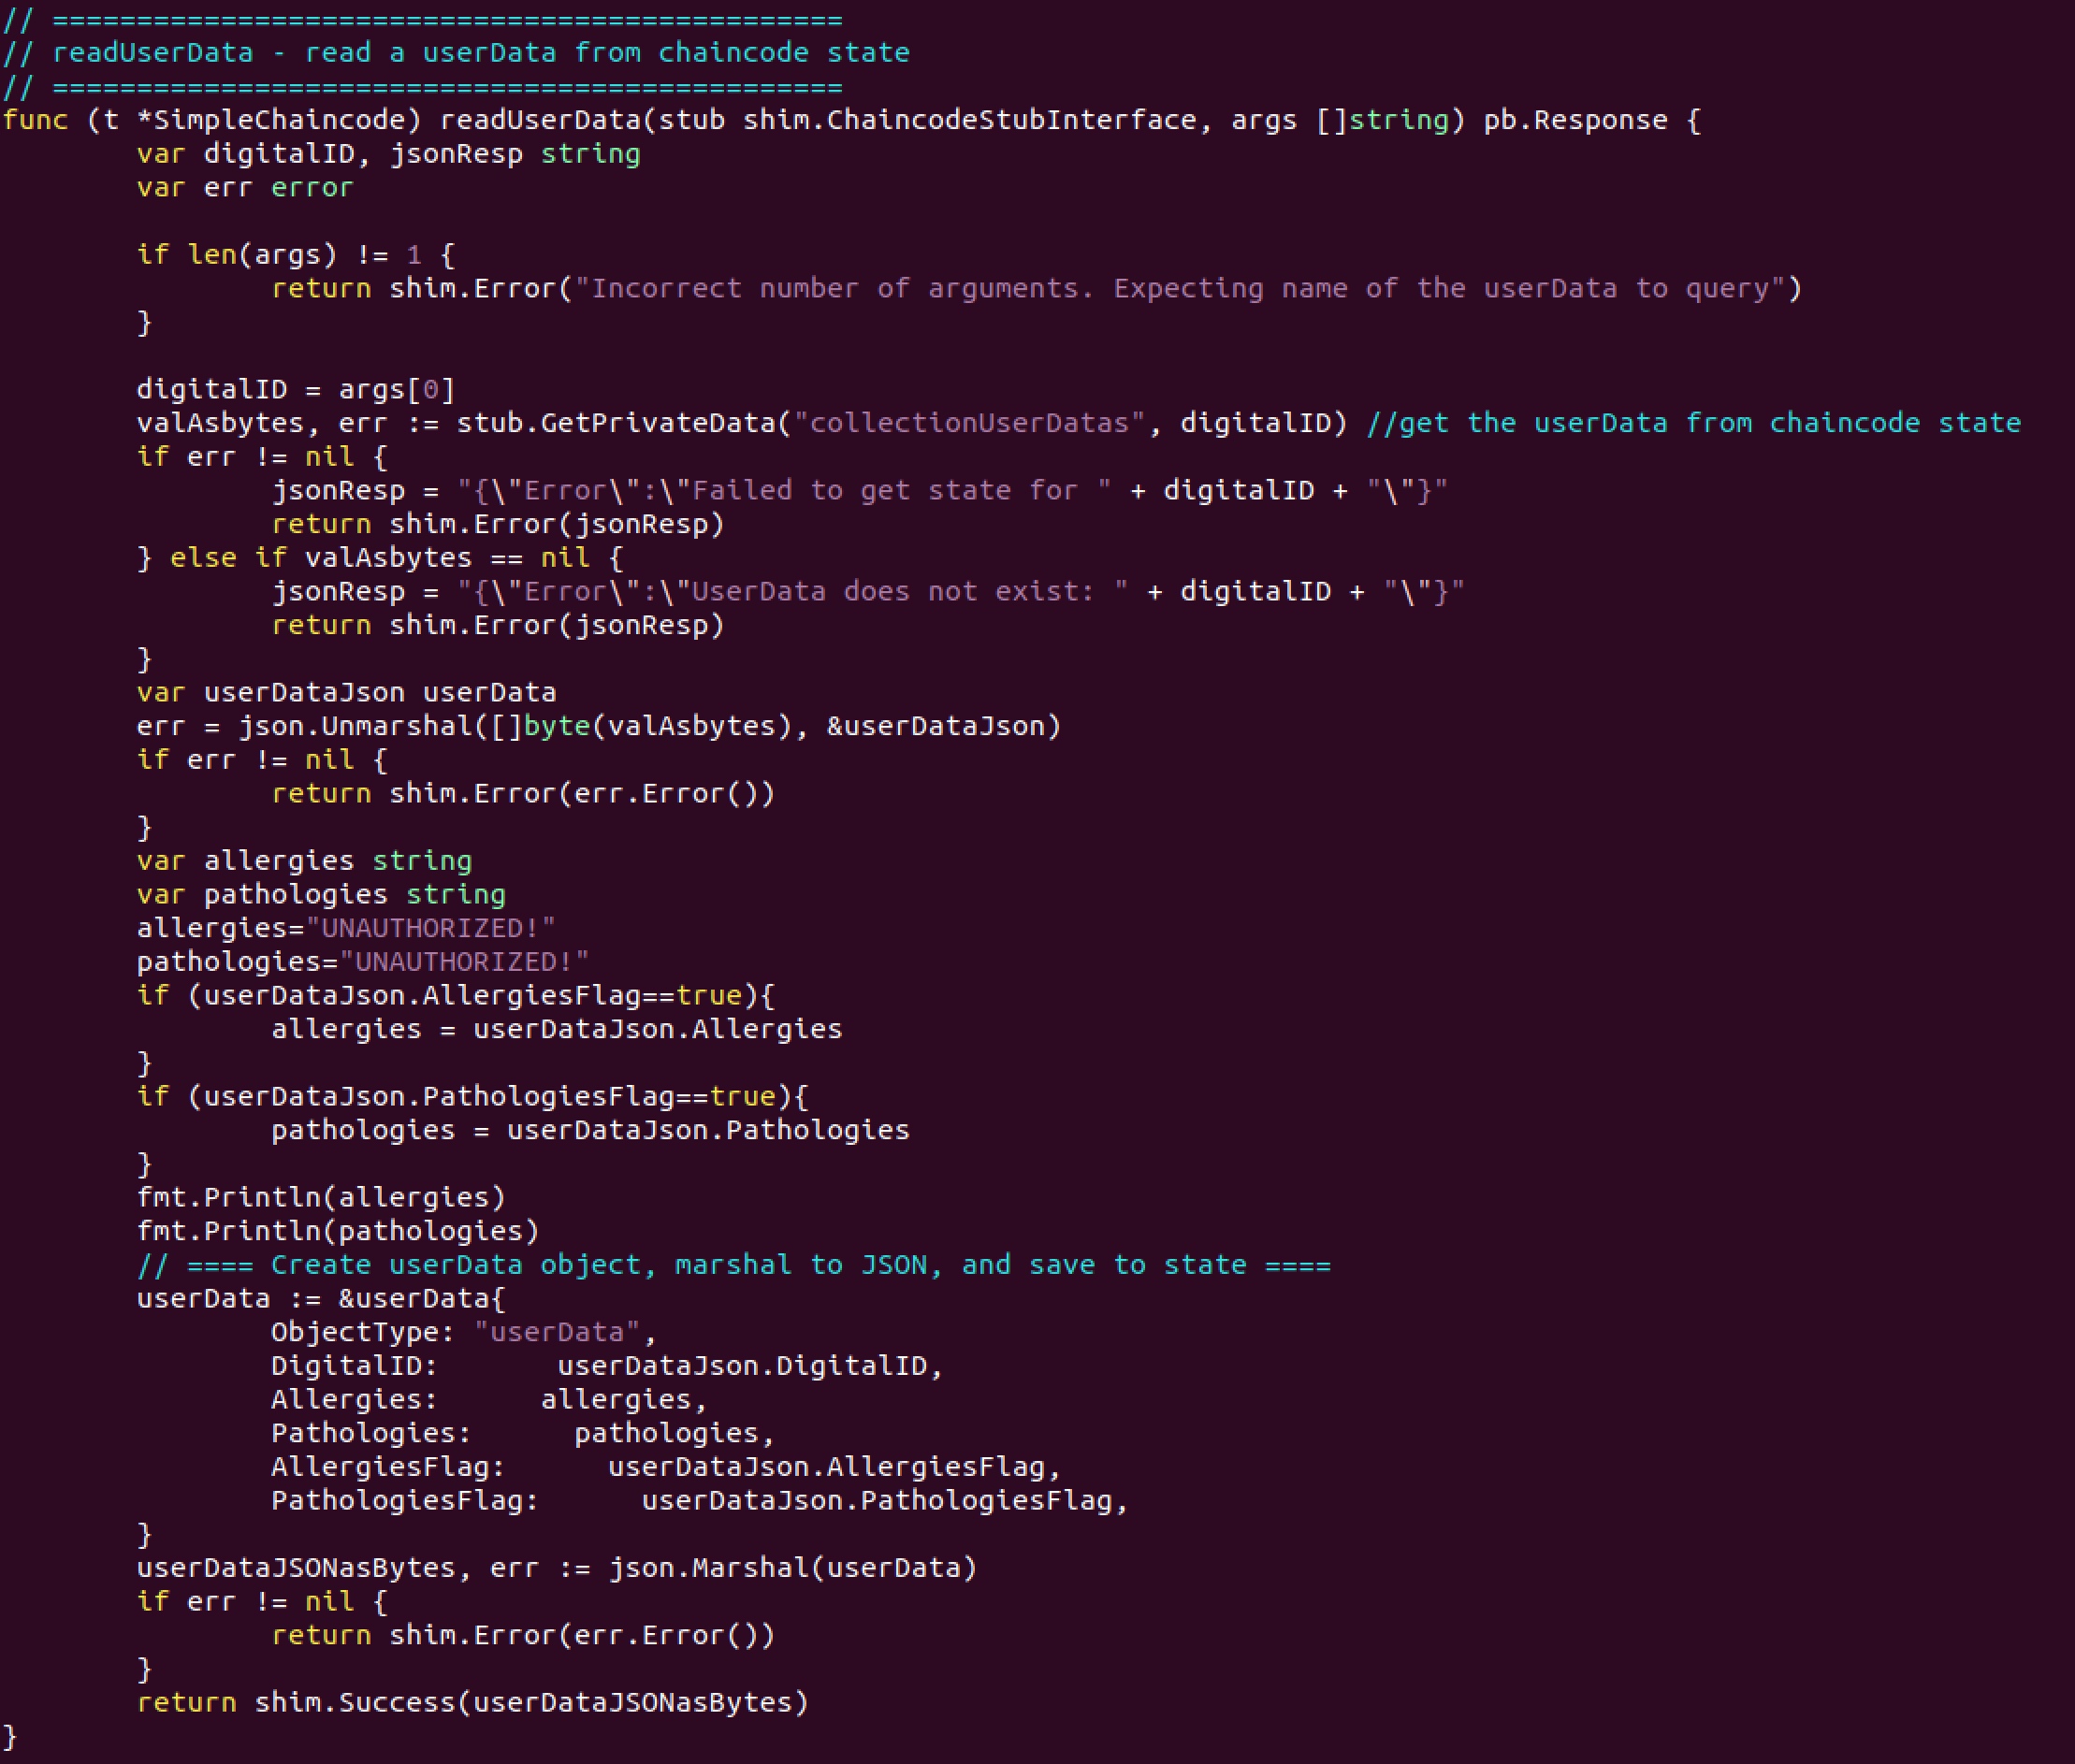
\includegraphics[width=1\textwidth]{img/function-chaincode.png}
    \caption{Funzione di lettura dei dati pubblici nel chaincode del caso sanitario}
    \label{fig:function-chaincode}
\end{figure}
\newpage
\section{Evoluzione del progetto}
Partendo dai prototipi sviluppati, possiamo ipotizzare che il prossimo step implementativo sia quello di adattare l'architettura formata da due organizzazioni a una più affine alla gestione logica degli attori dei due casi d'uso, andando a specificare un'organizzazione per ogni tipo di attore. Altre caratteristiche da poter migliorare sono quelle legate al sistema d'identificazione e di autenticazione andando a sostituire gli UUID autogenerati del prototipo con ID generati da un servizio di riconoscimento facciale.
\newpage
\voidpage
\chapter{Conclusione}
In conclusione possiamo dire che le blockchain sono molto interessanti per una gestione alternativa sui dati privati all'interno di settori come quelli bancari e finanziari. Anche la sicurezza, i trasporti urbani, così come il comparto della beneficienza, della fabbricazione, del monitoraggio e sanitario potrebbero essere trasformati dal più vasto impiego dei registri distribuiti su cui si basa l'architettura sperimentata.
Gli analisti, negli ultimi anni, sono arrivati a ipotizzare che gran parte delle industrie potrebbe trarre benefici più o meno eclatanti dall’impiego dei distributed ledger. Ci sono parecchi casi di utilizzo commerciale delle blockchain, con transazioni che vengono automaticamente verificate e organizzate da una piattaforma decentralizzata che non richiede la supervisione di un ente o di un soggetto centrale (super partes), pur garantendo la resistenza a manomissioni e frodi. Usi di tale genere possono essere facilitati tramite l'impiego di progetti come quelli basati su Hyperledger Fabric che, in molti contesti, facilitano la gestione della struttura dell'architettura e della logica di business sia sotto un punto di vista programmatico che applicativo. Infine, l'utilizzo di Hyperledger Fabric riesce a gestire programmaticamente e in totale semplicità tutte le operazioni di base per il rispetto dei criteri apportati all'interno della GDPR, tale caratteristica ha fatto si che molte aziende si interessassero all'adattamento della propria infrastruttura verso tecnologie innovative come quelle offerte dai progetti del dominio di Hyperledger.
\newpage
\voidpage
\pagestyle{plain}


\bibliographystyle{plain}
\bibliography{references}
\begin{thebibliography}{9}
\bibitem{Data Management}
\textit{ZeroUnoWeb - Sicurezza informatica, cioé disponibilità, integrità e riservatezza dei dati}
\\\texttt{https://www.zerounoweb.it/analytics/data-management}
\\\texttt{/sicurezza-informatica-cioe-disponibilita-integrita-}
\\\texttt{e-riservatezza-dei-dati/}

\bibitem{Rapporto Clusit 2019}
\textit{Rapporto Clusit 2019 - Associazione Italiana per la sicurezza informatica}
\\\texttt{https://clusit.it/rapporto-clusit/}

\bibitem{Regolamento generale sulla protezione dei dati}
\textit{GDPR - Regolamento generale sulla protezione dei dati}
\\\texttt{https://it.wikipedia.org/wiki/Regolamento\_generale\_sulla\_protezione\_dei\_dati}

\bibitem{Definizione di blockchain}
\textit{Blockchain: cos’è, come funziona e gli ambiti applicativi in Italia}
\\\texttt{https://www.blockchain4innovation.it/esperti/}
\\\texttt{blockchain-perche-e-cosi-importante/}

\bibitem{Categorizzazione delle blockchain}
\textit{Spindox - La classificazione delle Blockchain}
\\\texttt{https://www.spindox.it/it/blog/la-classificazione-delle-blockchain/}

\bibitem{Gestione della transazione}
\textit{CriptoInvestire - Mining: Come funziona la verifica delle transazioni}
\\\texttt{https://www.criptoinvestire.com/mining-come-funziona-}
\\\texttt{la-verifica-delle-transazioni.html}

\bibitem{Proof of Work and Proof of Stake}
\textit{Binance Academy - Proof of Work vs Proof of Stake}
\\\texttt{https://www.bitdegree.org/tutorials/proof-of-work-vs-proof-of-stake/}

\bibitem{Hard and Soft Fork}
\textit{Binance Academy - Hard and Soft Fork}
\\\texttt{https://www.binance.vision/it/blockchain/hard-forks-and-soft-forks}

\bibitem{Protocollo HTTP}
\textit{Hypertext Transfer Protocol - Wikipedia}
\\\texttt{https://it.wikipedia.org/wiki/Hypertext\_Transfer\_Protocol}

\bibitem{Linguaggio Go}
\textit{Tesi di Fabrizio Tonus, Ingegneria Informatica,\newline}
\textit{Università degli Studi di Padova - Il linguaggio di programmazione Go}
\\\texttt{http://tesi.cab.unipd.it/33111/1/Tesina\_562011.pdf}

\bibitem{Documentazione Node.js}
\textit{Informazione Node.js - OpenJS Foundation}
\\\texttt{https://www.html.it/articoli/cos-e-rest-caratteristiche/}

\bibitem{REST API}
\textit{Tutti quanti voglion fare REST, HTML.it - Andrea Chiarelli}
\\\texttt{http://html.it/articoli/cos-e-rest-caratteristiche/}

\bibitem{Express.js}
\textit{Node ed Express per applicazioni lato server - Davide Copelli}
\\\texttt{https://www.video-corsi.com/creareapp/node\_ed\_express\_per\_app\_lato}
\\\texttt{\_server}

\bibitem{Libreria Shim}
\textit{GoDoc - Documentazione sulla libreria shim}
\\\texttt{https://godoc.org/github.com/hyperledger/fabric-chaincode-go/shim}

\bibitem{Hyperledger Fabric}
\textit{Hyperledger Fabric - Documentation}
\\\texttt{https://hyperledger-fabric.readthedocs.io/en/latest/}

\bibitem{Docker}
\textit{RedHat - Cos'è Docker?}
\\\texttt{https://www.redhat.com/it/topics/containers/what-is-docker}

\bibitem{REST API per il server}
\textit{Hyperledger Fabric: Extending the FabCar network with ExpressJS REST API}
\textit{ - Kruk Matias}
\\\texttt{https://medium.com/coinmonks/hyperledger-fabric\newline-extending-the-fabcar-example-with-a-expressjs-rest-api-c270710ebbc}
\end{thebibliography}
\end{document}


